%
% The Current Maintainer of this work is Paul Vojta.

\documentclass[masters]{ucbthesis}
\usepackage{biblatex}
\usepackage{color}
\usepackage{graphicx}
\usepackage{subcaption}
\usepackage{siunitx}
\usepackage{listings}
\usepackage{rotating}
\usepackage{multirow}

% To compile this file, run "latex thesis", then "biber thesis"
% (or "bibtex thesis", if the output from latex asks for that instead),
% and then "latex thesis" (without the quotes in each case).

% Double spacing, if you want it.  Do not use for the final copy.
\def\dsp{\def\baselinestretch{1.5}\large\normalsize}
\dsp

% If the Grad. Division insists that the first paragraph of a section
% be indented (like the others), then include this line:
% \usepackage{indentfirst}

% Helpful commands
\newcommand{\TODO}[1]{{\color{red}\textbf{TODO: #1}}}
\newcommand{\RISCV}{\mbox{RISC-V}}
\bibliography{refs}


% Increase the depth of numbering sections

\hyphenation{Rocket-Chip MIDAS}
\begin{document}

% Declarations for Front Matter

\title{An FPGA-Hosted Configurable Off-Chip Memory Model}
\author{David Thomas Biancolin}
\degreesemester{Spring}
\degreeyear{2017}
\degree{Master of Science}
\chair{Professor Krste Asanovi\'c}
\othermembers{Professor Jonathan Bachrach}
\numberofmembers{2}
% Previous degrees are no longer to be listed on the title page.
% \prevdegrees{B.A. (University of Northern South Dakota at Hoople) 1978 \\
%   M.S. (Ed's School of Quantum Mechanics and Muffler Repair) 1989}
\field{Electrical Engineering and Computer Science}
% Designated Emphasis -- this is optional, and rare
% \emphasis{Colloidal Telemetry}
% This is optional, and rare
% \jointinstitution{University of Western Maryland}
% This is optional
\campus{Berkeley}

% For a masters thesis, replace the above \documentclass line with
% \documentclass[masters]{ucbthesis}
% This affects the title and approval pages, which by default calls this
% document a "dissertation", not a "thesis".

% A slightly modified template of the ms thesis to reuse the title variables
\clearpage
\makeatletter
\thispagestyle{empty}

\begin{center}
\rule{6.5in}{0.40mm}

\vspace{0.35in}
    {\large \textbf{\@title} }

\vspace{0.25in}
    {\large by \@author }

\vspace{0.35in}
\rule{6.5in}{0.40mm}

\vspace{0.5in}
    {\large {\textbf{Research Project}}}
\end{center}

\noindent Submitted to the Department of Electrical Engineering and
Computer Sciences, University of California at Berkeley,
in partial satisfaction of the requirements for the degree
of \textbf{Master of Science, Plan II}.

\vspace{0.25in}
\noindent Approval for the Report and Comprehensive Examination:

\begin{center}
    \textbf{ Committee:}

\vspace{0.25in}
\rule{3.5in}{0.25mm}

\@chair

Research Advisor

\vspace{0.25in}
\rule{3.5in}{0.25mm}

(Date)

\vspace{0.25in}
* * * * * * *

\vspace{0.25in}
\rule{3.5in}{0.25mm}

\@othermembers

Second Reader

\vspace{0.25in}
\rule{3.5in}{0.25mm}

(Date)
\end{center}
\makeatother

\maketitle
% Delete (or comment out) the \approvalpage line for the final version.
%\approvalpage
%\copyrightpage

%Recent work in FPGA-accelerated simulation of ASICs has shown that much
of a simulator can be automatically generated from ASIC RTL.  Alas, these works rely on simple models of
the outer cache hierarchy and DRAM, as
mapping ASIC RTL for these components into an FPGA fabric is too
complex and resource intensive.  To improve FPGA simulation model
accuracy, we present \PNAME~(FPGA-Accelerated Simulation and Evaluation of DRAM), a
parameterized generator of composable, high-fidelity, FPGA-hosted
last-level-cache and DRAM models. \PNAME instances are highly
performant, yet they maintain timing faithfulness independently of the
behavior of the host-FPGA memory system.
For a given scheduling policy, a single \PNAME instance can model
nearly the entire space of realizable single-channel DDR3 memory
organizations, without resynthesizing the simulator RTL.
We demonstrate \PNAME by integrating it into a flow that automatically
transforms RTL for multicore RISC-V processors into full-system
simulators that execute at up to 150 target MHz on cloud-hosted FPGAs.


\begin{frontmatter}

% You can delete the \clearpage lines if you don't want these to start on
% separate pages.

\setcounter{tocdepth}{2}
\setcounter{secnumdepth}{2}
\tableofcontents
\clearpage
\listoffigures
\clearpage
\listoftables

\begin{acknowledgements}
\end{acknowledgements}

\end{frontmatter}

\pagestyle{headings}

% (Optional) \part{First Part}

\chapter{Introduction}
\chapter{Introduction}



\chapter{A Renewed Case for FPGA-Accelerated Simulation}
% This section describes historical and related FPGA simulation work, and aims
% to call out techniques employed by this paper, in addition to describing
% problems with those works

We first review the use of FPGAs for architecture studies.  Throughout
this paper, we make a distinction between the \emph{target} and
the \emph{host}.  The target is the design under study.  Combining the
target with a model of the environment in which it executes forms a
determinate closed system whose behavior is defined independently of
the simulation host.  The host is the hardware that
executes~(\emph{hosts}) the simulation.  In this paper, a host
consists of one or more CPUs connected to one or more FPGAs.

\section{FPGA Prototyping}
FPGAs have long been used to \emph{prototype} ASICs by implementing
the ASIC RTL directly in FPGA logic.  While FPGA prototypes are both
fast~(10s to 100s of MHz) and detailed, they require a complete RTL
description of the target design. Furthermore, larger designs must be
painstakingly partitioned across multiple FPGAs. Since these
multi-FPGA prototypes advance in lockstep, cycle by cycle, they are
considerably slower~(100s of KHz to 1s of MHz). Nonetheless, FPGAs are used widely
in industry, as they allow software development and hardware
validation to proceed months before silicon is available.

\section{FPGA-Accelerated Simulation}

Prior work has explored techniques to make FPGAs more usable and
powerful simulation hosts.  Motivated by the dawn of the multicore
era, the multi-university RAMP project~\cite{RAMP} made large strides
in improving FPGA-accelerated simulators by improving resource
efficiency, developing FPGA partitioning techniques, and avoiding FPGA
recompilation by using reconfigurable models.

ProtoFlex~\cite{protoflex} was an architecture-level simulator that
demonstrated 16-way host-multithreading of a single FPGA-hosted functional model.
ProtoFlex could switch between FPGA-hosted and CPU-hosted modes via
\emph{transplantation}. FAST~\cite{FAST}, a cycle-accurate simulator, was
split into CPU-hosted functional and FPGA-hosted timing models.  RAMP
Gold~\cite{RAMPGold} used FPGA-hosted timing and functional models
with 64-way host-multithreading to model a larger target on a single
FPGA.  HAsim~\cite{HASIM} also used FPGA-hosted timing and functional
models, but provided more detailed pipeline and memory hierarchy
models.

Other work studied partitioning targets over multiple FPGAs.
\cite{LIFPGADesign} showed that by partitioning HAsim over two FPGAs, they
could model eight times as many cores, due to improved resource sharing between
virtual instances. To model a datacenter-scale target, DIABLO~\cite{Diablo}
leveraged RAMP Gold's multithreading to simulate 3072 servers on 24 FPGAs.

A unifying theme of FPGA-accelerated simulators is that one clock-cycle of
target time is executed over a variable number of FPGA-host
cycles.  This lets an FPGA-hosted simulator hide
variable host latencies to DRAM and CPU-hosted components, enables
optimizations that trade host time for host resources, and, crucially,
facilitates deterministic simulation.  This \emph{host-target
decoupling} is what differentiates an FPGA-accelerated simulator from
an FPGA prototype. We expand on this property in
Section~\ref{sec:fame1}.

\section{Adoption Challenges}

Despite their promise, FPGA-accelerated simulators have only been
successfully employed by those who designed them. We attribute their
limited appeal to several factors:

\begin{enumerate}

    \item \textbf{Availability.} Much of the early FPGA-accelerated
    simulator research relied on boutique FPGA-emulation
    platforms or custom board designs, whose high cost and
    limited availability prevented adoption.

    \item \textbf{FPGA Capacity.} Common ASIC structures, such as CAMs and
        multi-ported RAMs, map poorly to FPGA
        fabrics~\cite{FPGAGap2}, making it difficult to host large
        ASIC designs on FPGAs.

    \item \textbf{Ease of Use.} To avoid partitioning across multiple
     FPGAs, previous work focused on efficiently mapping more of the
     target to a single FPGA. The abstract, multithreaded models these
     simulators typically employ can be more difficult to implement
     than the machines they model, greatly undermining their
     usability. This complexity limits configurability, forcing users
     to modify a sophisticated piece of RTL to make larger
     changes. Furthermore, these abstract models must, like their
     software counterparts, be validated and calibrated, making them
     even more laborious to use.
\end{enumerate}

\section{Recent Technological Advances}

Even as Moore's law wanes, FPGA capacity continues to scale. The largest FPGAs
have over \wunits{50}{MiB} of BRAM and millions of logic cells.
%\footnote{Scaling RAMP
%Gold~\cite{RAMPGold} to use the largest Xilinx UltraScale+
%FPGA~\cite{Ultrascale} would permit modeling more than 5000 cores!}
As they
have scaled, FPGAs have become more heterogeneous, adding features that make
them better hosts for full-system simulators.  Both Intel and Xilinx sell FPGAs
with embedded microprocessors, making it easier to co-simulate tightly coupled
hardware and software models. Modern FPGAs include dedicated DRAM
controllers that support memory bandwidths rivaling those of ASICs.

Lower cost and increased on-chip integration have also made FPGAs more
accessible to researchers.  Not only are commercial off-the-shelf development
boards cheaper and more full-featured, FPGAs are now available as a cloud service~\cite{amazonf1}.
Where in the past academics would have to purchase their own FPGAs to reproduce
published experiments, instead, it is now possible to spin up identical
simulations on FPGAs in the cloud.  This development promises to foster more
collaboration around FPGA-accelerated simulation.

\section{Usability Through Automation}

While the trends described in the previous section solve the
\emph{availability} and \emph{FPGA capacity} challenges, usability remains a
problem. Previous work~\cite{fabscalarfpga, strober} has shown that much of an
FPGA-accelerated simulator can be automatically generated from source RTL. This RTL
can be written in an HDL like Verilog, generated by a high-level synthesis
tool, or emitted by languages like Chisel~\cite{Chisel} or Bluespec.

Alas, it is not always practical to generate models from source
RTL. Consider off-chip memory systems: they are too resource-intensive to host
in the FPGA fabric, yet for reasonable simulation performance, they must be
tightly coupled with the processor model.  Components like these require
an abstract model to virtualize the target memory system over DRAM attached
to the FPGA---reintroducing the problem that anything
but a simplistic model is difficult to design, validate, modify, and reuse.

To avoid these pitfalls, we propose writing detailed memory-system
timing models as decoupled, split-timing-and-functional models with
the timing models written as \emph{target-time} RTL. Using this
approach, the same RTL transformations applied automatically to the
processor RTL are applied to the timing-model RTL before binding it to
the functional model.  Model designers can focus on modeling detailed
target behavior and not worry about the mapping to the host.  With our
approach, since timing models are transformed from target-time RTL, it
is possible to use HLS-generated RTL or even existing
memory-controller RTL as a timing model.

To improve reusability, we propose writing timing models
as \emph{generators}.  This allows the model designer to describe a
space of \emph{instances} with less development effort.  To
support reconfiguring timing models without FPGA recompilation, timing
models expose timing parameters as I/Os that are bound automatically
to memory-mapped registers during timing-model generation.  Taken
together, these techniques make it possible to describe
detailed, reusable memory-system models.  We demonstrate this claim with \PNAME.


\chapter{A Primer on MIDAS}
We prototype our models in an FPGA-Accelerated simulation framework that builds on
the Rocket-Chip \cite{rocketchip} infrastructure (similar to
\cite{strober}). Our designs are developed in Chisel, a high-level
hardware-description language written in Scala. Building on this infrastructure
allows us to leverage a large amount of available open-source IP and a growing
software ecosystem that includes GCC, Linux and LLVM.

Our framework makes use of FIRRTL~\cite{firrtl}, an intermediate representation
(IR) for RTL that has frontends for both Chisel and Verilog, and can target
both FPGA and ASIC flows by emitting optimized Verilog output. FIRRTL enables
the implementation of compiler passes on top its IR framework. These passes
can, for example, apply FPGA-optimizations, add instrumentation, and
automatically produce scan chains for debugging and power
estimation\cite{strober} -- all without requiring modifications to the source
RTL.

\begin{figure}
	\centering
	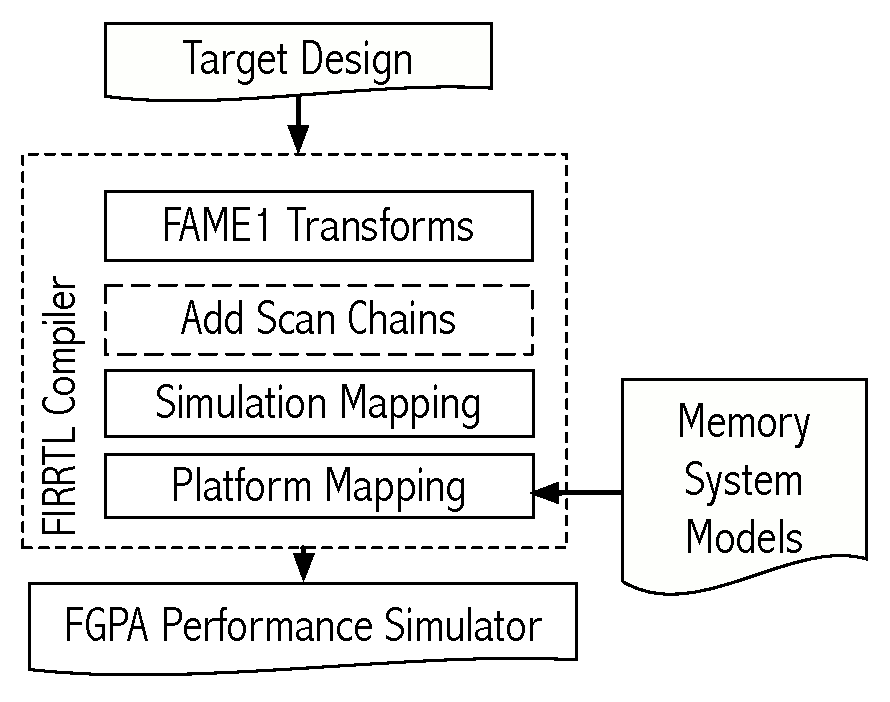
\includegraphics[width=7cm]{figures/firrtl.pdf}
	\caption{FIRRTL custom transforms for the FPGA simulator}
	\label{fig:firrtl}
\end{figure}


\section{Host-Target Decoupling in MIDAS}

\section{Transformations of Source RTL}

MIDAS uses FIRRTL compiler passes to preform transformation source RTL into
host-decoupled models. The most important of these is the FAME-1
transformation, which adds to requsite logic to host-decouple target RTL, so
that it may conform to a RAMP model of execution. \TODO{See Section}. In figure
\TODO{Auto-transformation} below, the procedure through which source RTL is
host decoupled is illustated.


Additional transformations may be invoked to add scan
chains and I/O trace buffers for debugging, and for state snapshotting for use
with Strober\cite{strober}.

\section{Platform Mapping}

\section{Target Machines}

While this approach is applicable to arbitrary RTL, one challenge lies in
sourcing the RTL to build a realistic target. While we build on RocketChip and
\RISCV, our approach could in principle be used with other open-source designs
such as OpenPiton\cite{openpiton} and FabScalar\cite{fabscalar}.


\chapter{An Overview of DRAM Off-Chip Memory Systems}
\section{DRAM Device Architecture}\label{sec:dram-arch} In a DRAM IC, arrays of
bit cells are hierarchically arranged into multiple parallel \emph{banks}.
Banks provide the primitive level of concurrency in a DRAM memory system. They
can service independent requests, assuming they do not simultaneously require
shared resources like the data, address and command buses.  Multiple DRAM ICs
can be arranged in parallel to widen the data bus; address and command buses
fan out to each IC. For more concurrency, and to support larger memory
capacities, multiple \emph{ranks} of DRAM devices may be used. Here, generally,
the command and data buses are shared between all ranks, with a one-hot
chip-select indicating which rank a command is addressed to.

A basic DRAM operation requires a series of three commands: \emph{activate
(ACT)}, \emph{column access~(CAS)}, and \emph{precharge~(PRE)}. The ACT command
enables the word-lines of the array corresponding to a single \emph{row} of the
bank. The cells of the row are sensed and saved in a \emph{row
buffer}(typically 1-2 kB). A CAS command then selects a subset of the row
buffer to read or write~(CASR and CASW commands respectively). In double-data
rate~(DDR) DRAM, data is bursted over successive rising and falling clock
edges.  While the row buffer remains \emph{open}, the row can be accessed by
issuing new CAS commands. To access a row not stored in the buffer, a PRE
command must be issued to \emph{close} the row and charge the bit lines for a
new access.

DRAM is named dynamic-RAM because it gradually loses its stored state over time
as bit-cell capacitors leak. DRAM-cell retention rates vary on a single die and
between dies and are highly sensitive to temperature~(warmer cells leak
faster). To maintain their state, DRAM cells must be periodically ``refreshed".
Activating a row of cells is sufficient to refresh them: the stored state is
read by the sense amplifiers and fed back into the bitlines at the supply
voltage, recharging the still-open capacitors.  As part of the DRAM standards,
JEDEC mandates cells must be refreshed on-average once every 8ms; an interval
they have maintained from DDR through DDR4. Since activations to every row
cannot generally be guaranteed, DRAM devices are refreshed explicitly with
a refresh command~(REF). To reduce complexity, this command refreshes a constant
number of contiguous rows beginning at a base row address in all banks
concurrently. The base address is incremented which each REF command. DRAM manufacturers generally
have kept the number of refresh commands required to iterate through the entire
array constant: 8192 commands per 8ms interval, or one on average every 64 $\mu s$.
Hence, refresh commands take longer to execute on denser devices with more rows
per bank.

A complete list of timings required to model a generic DDR protocol is give in
table \ref{tbl:dram-timings}. These have been taken, with some modification,
from \textit{Memory Systems: Cache, DRAM, Disk}\cite{drambook}.

\begin{table}[htb]
\begin{center}
\resizebox{\textwidth}{!}{%
    \begin{tabular}{|p{0.20\textwidth}|p{0.8\textwidth}|}
    \hline
    \textbf{Name} & \textbf{Description} \\
    \hline
    \hline
    \textbf{$t_{AL}$} & Additive Latency. Additional latency added to column access commands. \\
    \textbf{$t_{CAS}$~($t_{CL}$)} & Column Access Strobe latency. Delay between
    when a CASR command is received and when the first beat of read data is
    returned. \\ \textbf{$t_{CCD}$} & Column-to-Column Delay. Minimum duration
    between two consecutive column commands. \\ \textbf{$t_{CMD}$} & Command
    transport duration. The duration a command occupies the command bus. \\
    \textbf{$t_{CWD}$~($t_{WL}$)} & Column Write Delay. The delay between a
    CASW command and the when the controller must present the first beat of
    write data. \\
    \textbf{$t_{FAW}$} & Four row Activation Delay. A rolling time window
    during which only four row activations may be made to all banks of a DRAM
    device. \\
    \textbf{$t_{RAS}$} & Row Access Strobe. The minimum duration after an ACT
    command that the row must be kept open before issuing a precharge command
    to close it. \\
    \textbf{$t_{RC}$} & Row Cycle time. The minimum duration required
    to open, and close a row. $t_{RC} = t_{RAS} + t_{RP}$ \\
    \textbf{$t_{REFI}$} & Refresh Interval. The average period of time between refresh commands. \\
    \textbf{$t_{RCD}$} & Row-to-Column Delay. The minimum duration after
    activation column commands may be issued to the newly-opened row.  \\
    \textbf{$t_{RFC}$} & ReFresh Cycle time. The minimum duration after a refresh
    command that activation commands may be issued. \\
    \textbf{$t_{RP}$} & Row Precharge delay. The minimum duration after a
    precharge command that an ACT to the same bank may be issued. \\
    \textbf{$t_{RRD}$} & Row-to-Row Delay. The minimum duration between ACT commands to the same bank. \\
    \textbf{$t_{RTP}$} & Read-To-Precharge delay. The mimimum duration after a CASR command that a precharge may be issued to the same row. \\
    \textbf{$t_{RTRS}$} & Rank-To-Rank Switching delay. Accounts for time to change termination schemes on DQ and DQS buses when switching between ranks. \\
    \textbf{$t_{WR}$} & Write Recovery time. The minimum duration after a CASW command that a precharge command may be issued to the same row. \\
    \textbf{$t_{WTR}$} & Write TurnaRound Time. The minimum duration after a CASW command that a CASR may be issued to the same row. \\
    \hline
\end{tabular}}
\end{center}
\caption{A list of key timings for a conventional DDRx SDRAM}
\label{tbl:dram-timings}
\end{table}%

\clearpage
\section{DRAM Controller Architecture}

A DRAM controller is responsible for responding to memory
requests from one or more requestors by scheduling those requests over its
attached memories as a judicious stream of DRAM commands.

Memory access scheduling~(MAS) is the process by which, for a given cycle, a
controller selects a single DRAM command to be issued from a legal set. Legal
commands are constrained by the current state of each bank, the availability
of shared resources like the command and data buses, and timing constraints
imposed by the DRAM standard. Good MAS policies strike a delicate balance
between minimizing latency, maintaining quality-of-service guarantees across
multiple threads of execution, maximizing bandwidth, and minimizing power.
There are plethora of academic papers on MAS policies, and still more
industrial patents on the subject. In this work we consider two popular MAS policies. 

\subsection{First-Come First-Serve~(FCFS) Policy}\label{sec:fcfs} Commands for the
oldest pending memory reference are issued first. This is the simplest MAS
policy, but tends to under-utilize available DRAM bandwidth as younger requests
that may hit in the row-buffer are not issued before older commands that miss.
FCFS schedulers are common in older machines, and those that present few
concurrent memory requests.

\subsection{First-Ready FCFS~(FR-FCFS)~\cite{frfcfs} Policy}\label{sec:frfcfs}
First, ready~(legally issuable) column commands are prioritized over ready row
commands. Second, commands for older references are prioritized over younger
ones. This permits younger but ready column commands to be issued before older
row commands. FR-FCFS is a relatively simple scheme that improves bandwidth
utilization considerably. It is the de facto standard against which new MAS
policies for machines with a single stream of memory references~(like
single-core out-of-order machines), are compared.

\section{DRAM Software Simulation}

The current state of the art in DRAM simulation in academia are cycle-accurate
software simulators like DRAMSim2~\cite{dramsim}, Ramulator~\cite{ramulator} and
USIMM~\cite{usimm}. These models generate DRAM command streams that have been
validated against industrial models~(for some standards). Both Ramulator and
DRAMSim2 can be easily integrated into Gem5~\cite{gem5}, though gem5 includes a
detailed event-based model of its own~\cite{gem5event}. In trace-driven mode,
operating at full throughput and only as a timing-model, these cycle-accurate
models simulate at frequencies ranging from hundreds of KHz to ones of
MHz~\cite{ramulator}.

\section{DRAM Power Modeling}

In order to model power, Ramulator relies on DRAMPower~\cite{drampower}, to
which it passes its command trace. DRAMSim2 directly implements strategies
Micron has described in their technical notes~\cite{micronpower}. Micron has
also provided spreadsheets implementing these strategies, that take
microarchitectural event frequencies as input. These approaches can also be
used in an FPGA simulation, as sufficiently detailed FPGA models can add
instrumentation for specific events, while simpler models could save or sample
the memory access trace and compute power out-of-band.


\chapter{Memory Timing-Model Design}
% This section describes the design of the memory system model. How host target
% decoupling is achieved. What configurations are available.

Our memory timing-model \textit{generator} describes a space of
\textit{instances}, each of which may be used to model a space of
memory systems. As input, the generator accepts a configuration that specifies
the static parameters of the instance,  such as width of the interfaces it
binds to, the number of outstanding requests it must support, and the type of
memory system the instance will model (a \emph{timing-model class}). As output,
the generator produces an instance module and local memory map of all registers
it will expose to the simulation interconnect. These registers control timing
parameters can be overwritten to reconfigure the instance without needing to
recompile the FPGA bitstream.

Instances operate by using the FPGA-host's off-chip memory system as a backing
store: target requests carried through simulation tokens are snooped by the
\emph{ingress unit} and re-issued to the host-memory system. Responses from the
host-memory system are subsequently buffered by the \emph{egress unit}. In
parallel, a host-decoupled \emph{timing-model} explicitly consumes input tokens
and generates output tokens. When the timing-model wishes to release a token
with a valid target response, it fetches the matching host response from the
egress unit. If no host response is present, the timing-model does not produce
a token. This makes the behavior of the target-memory system independent of the
behavior of host-memory system, and thus, reproducible.

A block diagram of an instance is shown in figure~\ref{fig:timing-model}.

\begin{figure}
	\centering
	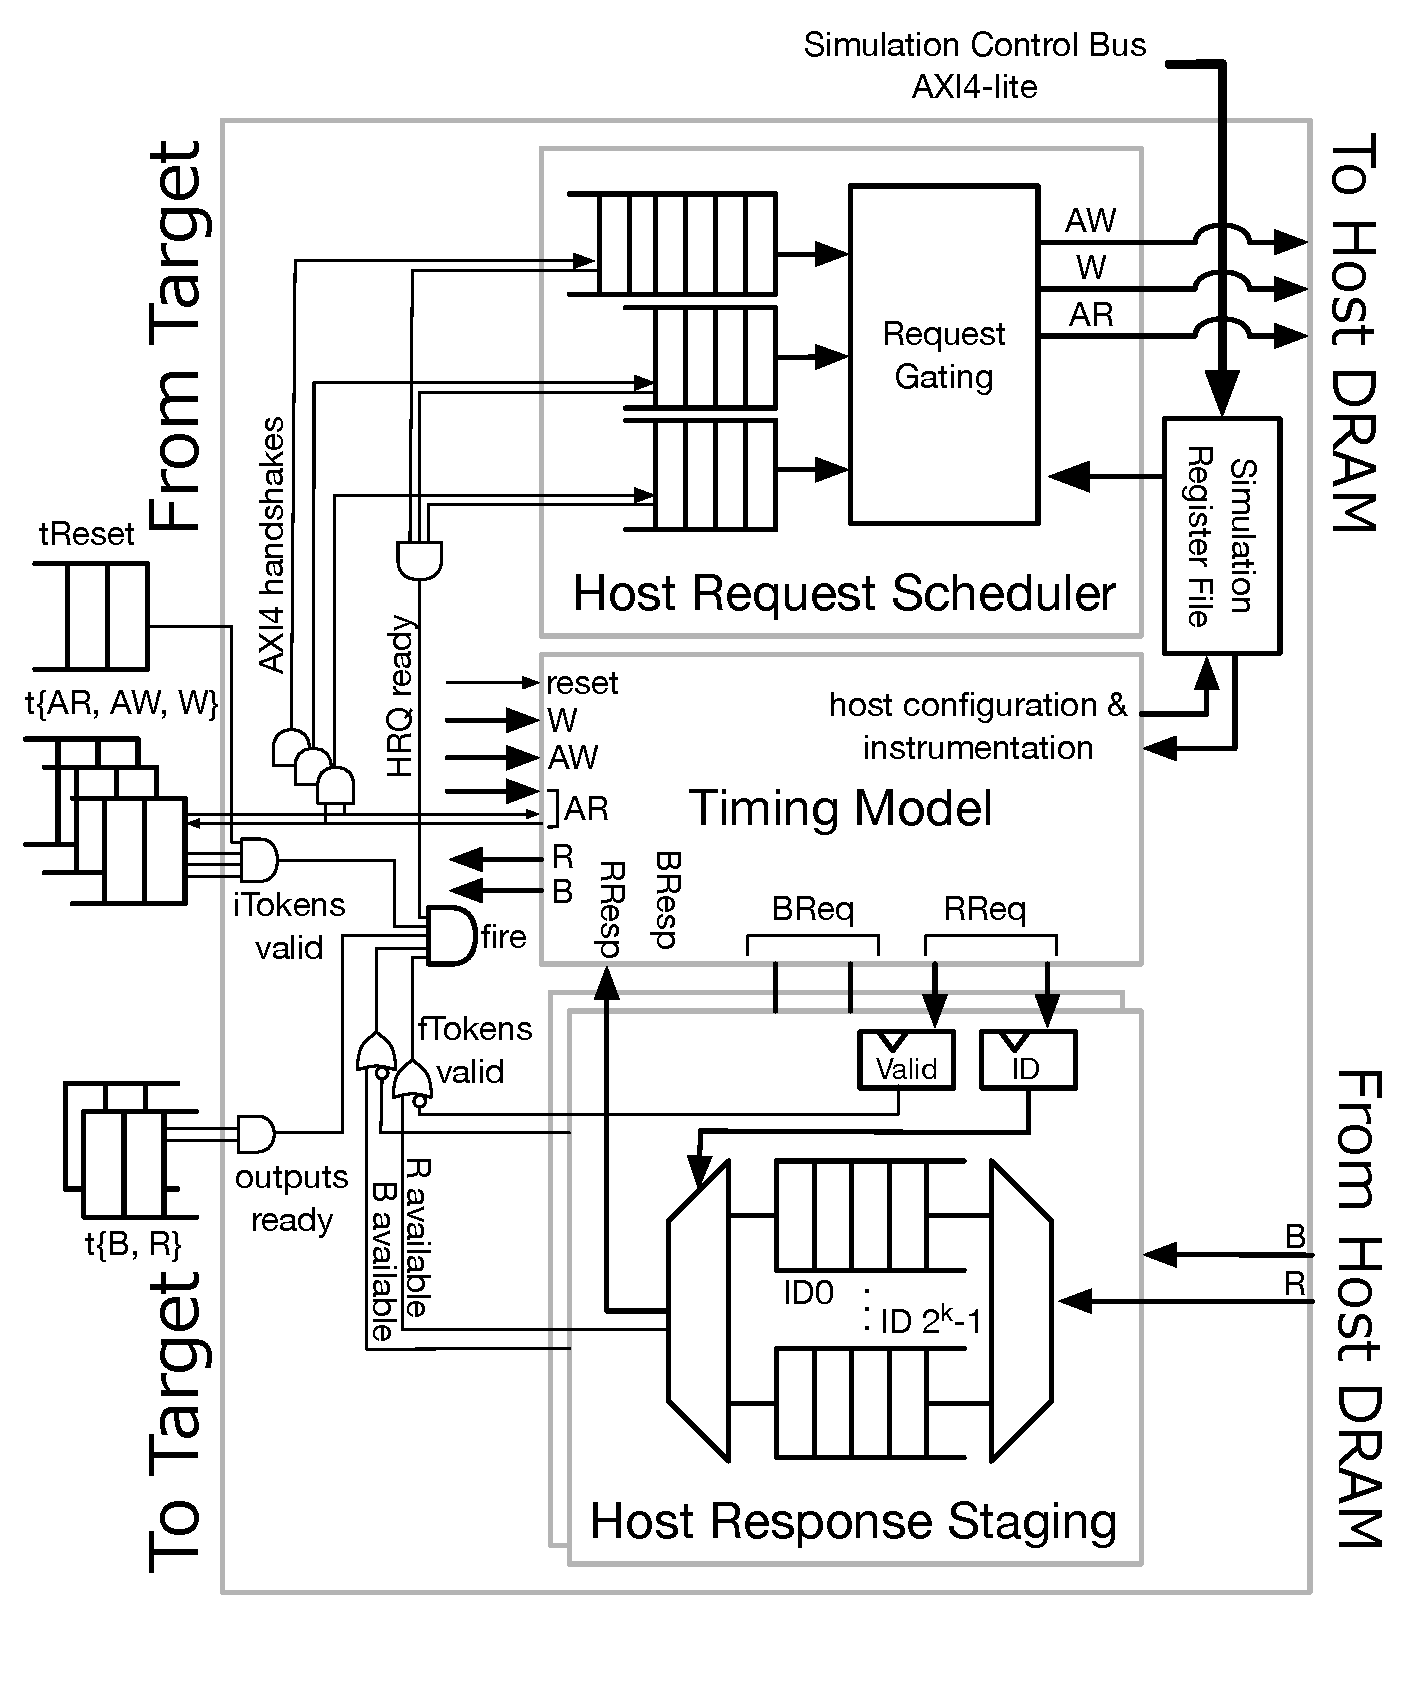
\includegraphics[width=\columnwidth]{figures/memory-model-block-diagram.pdf}
     % graffle2pdf -c full midas-graphics/graffle/memory-model-block-diagram.graffle figures/memory-model-block-diagram.pdf
    \caption{A block diagram of a \PNAME instance, with all control signals
    that may stall timing model execution illustrated.}
	\label{fig:timing-model}
\end{figure}

\section{Interfaces}\label{sec:interfaces}

All instances have three interfaces.

\begin{enumerate}
    \item \textbf{Target-side:} Host-decoupled AXI4 slave
        interface and synchronous reset. AXI4 consists of five ready-valid
        channels; three request channels driven by the master, and two
        response channels driven by the slave.  An input token consists of
        the valids and payloads for each request channel, the readies for
        each response channel, and the synchronous reset.  An output token
        is the complement; the valids and payloads for each response
        channel, and the readies for each request channel.  While tokens
        may be carried to and from the instance on separate timing channels
        (for each AXI4 channel and reset), simulation mapping ensures
        these are fused into a single input token, and fractured into
        multiple output tokens accordingly.

    \item \textbf{Host-side:} AXI4 master. This interface is used by the
        instance to make requests of the host-memory system. It operates
        independently of target-time.

    \item \textbf{Configuration-side:} AXI4-lite slave. This interface exposes both
        memory-mapped configuration registers and instrumentation to the
        simulation interconnect.

\end{enumerate}

We selected AXI4 as it is the most common bus standard presented by FPGA IP and
widely implemented in ASICs. On the host-side, both major FPGA vendors provide
IP to bridge AXI4 to other standards, as well as adapters to connect master
and slave devices that may have different interface widths. If the target does
not present an AXI4 master, the user will need to generate a bridge in their
source RTL or introduce a bridge model. In the future, we expect to include
target-side interfaces for other interface specifications, like TileLink.

The widths of all fields in target-side and host-side interfaces match. The
model punts all on all conversions, like target-to-host address translation,
which will be handled by the MIDAS compiler.

\section{Operation}\label{sec:operation}

Like most previous FPGA-simulation work using handwritten-RTL models, the instances
split their timing and functional models.

The functional model of an instance is comprised of the ingress unit, egress
unit and a host-memory region of sufficient size. While in general any sane
memory should be a viable functional model for another memory of equal size,
instances specifically use another AXI4 memory-slave component on the host as a
functional model for an AXI4 memory-slave component in the target. This makes
it trivial to apply target requests to the functional model; the instance need
not worry about translating requests between different bus standards. Instead,
the model relies on bridges and adapters in the host-memory system to manage
that complexity.

The ingress and egress unit are the gatekeepers of the host-memory system. They
apply target requests to the host-memory system and buffer responses so that
they may be fetched by the timing-model without violating AXI4 ordering
constraints. They must do this without locking up the host-memory system (more
on this later).

The ingress unit snoops the values of input tokens and outputs tokens. When the
timing model handshakes on a read address, write address or write data request,
it enqueues the payload of that request into a queue for that AXI4 channel. Once
the ingress unit has buffered a complete read or write transaction, it issues
it to the host-memory system. The ingress unit must wait until it has complete
transaction to avoid locking up the host-memory system in the case that
simulation halts during a target request, or if the target attempts to reset
the controller.  If any of the queues of the ingress unit would overflow, the
timing-model may not advance (it cannot dequeue input tokens). At minimum,
the queues must be sized to hold a single complete request to avoid deadlocking
simulation.\footnote{The minimums are ARQueue depth of 1, WQueue depth of
\emph{MaxWriteLength}, AWQueue depth of \emph{MaxWrites}, where MaxWriteLength
and MaxWrites are set in the base
configuration.(Section~\ref{sec:generator-parameters},
table~\ref{tbl:base-config}). The default is the same, but with ARQueue depth
increased to 4.} Adding additional buffering on the AR queue may increase FMR
by insulating the model against backpressure received from the host-memory
system.

The egress unit is responsible for buffering the pertinent fields of host
responses until they are requested by the timing-model. The egress unit must
rectify reorderings made by both the host-memory system and the timing-model.
In AXI4, there are two ordering constraints of concern for design of the  egress unit
design(see~\cite{amba}, section A6.4 for greater detail):

\begin{enumerate}

    \item Reads with the same AXI4 transaction ID must have their responses returned in the
        order in which the requests arrived.

    \item Writes with the same AXI4 transaction ID must have their responses returned in
        the order in which the requests arrived.\footnote{Reads and writes with
        the same AXI4 ID may be reordered.}

\end{enumerate}

To adhere to these constraints, the egress unit implements a \emph{virtual queue}
for each AXI4 ID, with separate sets both read and write responses. As host
responses are presented they are enqueued into the virtual queue with the
corresponding AXI ID. For read responses, the egress unit only buffers the data
and last fields of a read response payload.\footnote{The user signal (RUSER)
and read response status (RRESP) fields are dropped.} For writes, none of the
payload fields are enqueued; the queue degenerates into a up-down counter of
write acknowledgments it has received for each ID.\footnote{Write
acknowledgments do have WUSER and WRESP fields but, as above, they are
dropped.} The implementation of the virtual queues depends on generator
parameters described in section~\ref{sec:generator-parameters}. Details of the
various egress unit implementations are described in section~\ref{sec:egress}.

In parallel, the timing-model consumes input tokens and generates output
tokens. As described in section~\ref{sec:interfaces}, an output token includes
both the backpressure (ready) on request channels as well as the valid bits and
payloads of response channels. The timing-model is free to drive signals in the
read and write response payloads as it sees fit; it may wish to return custom
errors or hints, or even return incorrect data. Generally, for read responses
the timing-model fetches missing fields beat-by-beat from the egress unit,
whereas for write responses, it consumes a credit ensuring that the host write
response has been received.

To this end, the egress unit exposes ready-valid request and response
interfaces for both reads and writes. The timing-model fetches the oldest
response for a given AXI ID by providing the ID through the request interface.
After a request handshake, the egress unit returns the beats of the transaction
at the head of that ID's virtual queue through the response interface. The
timing-model then handshakes on each beat to dequeue them from the egress unit.
The egress unit will only accept a new request once it has presented the final
beat of the previous one.\footnote{This is a natural restriction, as the AXI4
specification does not permit read-response interleaving. In the future this
could be changed, to have the model request individual beats instead of whole
transactions.}

In the event that the host-memory system is slow, the egress unit cannot return
a valid response and thus the timing-model cannot populate a complete output
token. Local and downstream target-time stalls. Only once the egress unit
receives the response from the host-memory system and forwards through to the
timing-model will the timing-model enqueue the new output token, permitting
target time to advance.  In this way, host-decoupling is maintained. This
permits an instance to model physically unrealizable memory systems. For
example, one could model single cycle memory system to perform studies of the
target design with an ideal memory system. The operation of such a model in
figure~\ref{fig:model-operation}.

\begin{figure*}
	\centering
    \begin{subfigure}[t]{0.23\textwidth}
        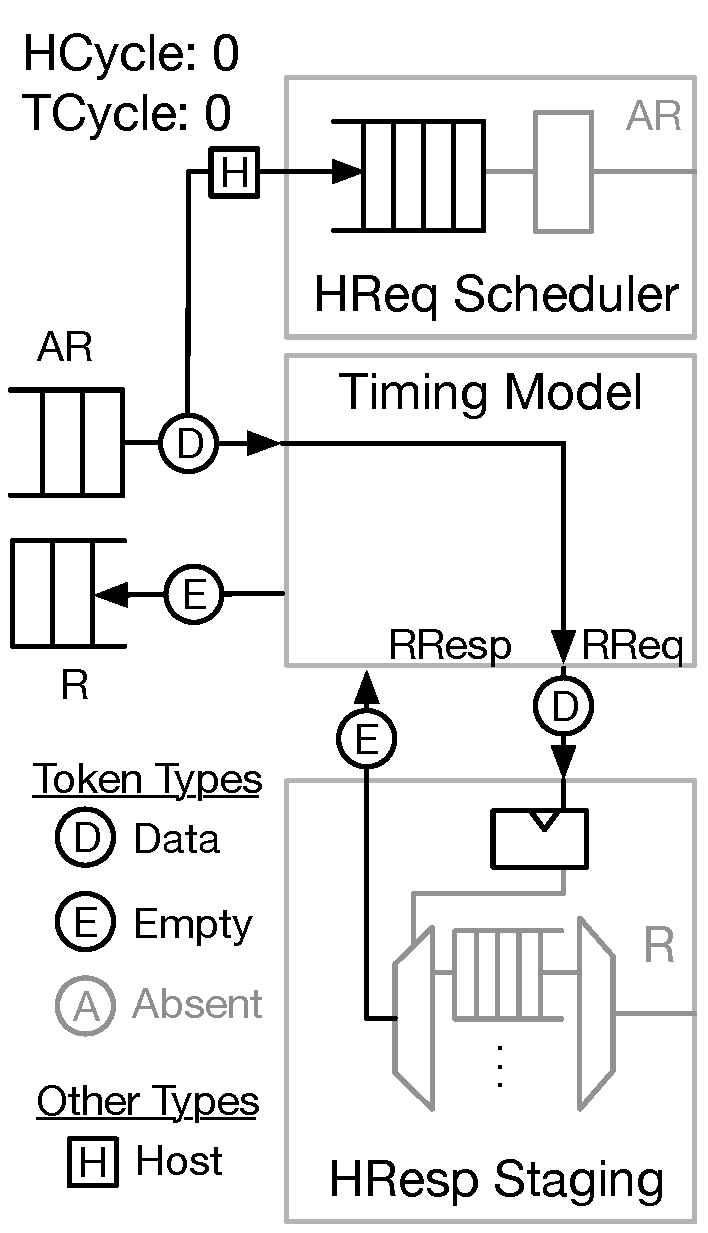
\includegraphics[width=\columnwidth]{figures/model-operation-1.pdf}
        % graffle2pdf -c 1 midas-graphics/graffle/memory-model-operation.graffle figures/model-operation-1.pdf
        \caption{}
        \label{fig:model-operation-1}
    \end{subfigure}
    \begin{subfigure}[t]{0.24\textwidth}
        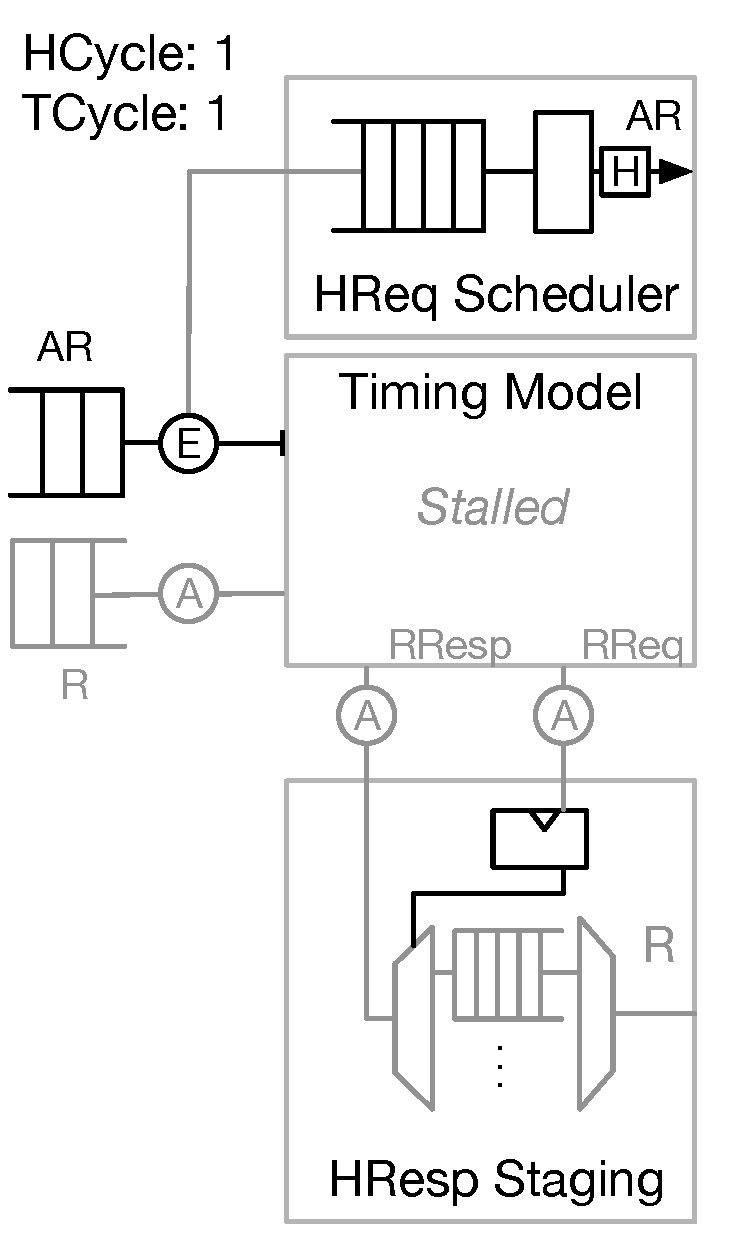
\includegraphics[width=\columnwidth]{figures/model-operation-2.pdf}
        % graffle2pdf -c 2 midas-graphics/graffle/memory-model-operation.graffle figures/model-operation-2.pdf
        \caption{}
        \label{fig:model-operation-2}
    \end{subfigure}
    \begin{subfigure}[t]{0.24\textwidth}
        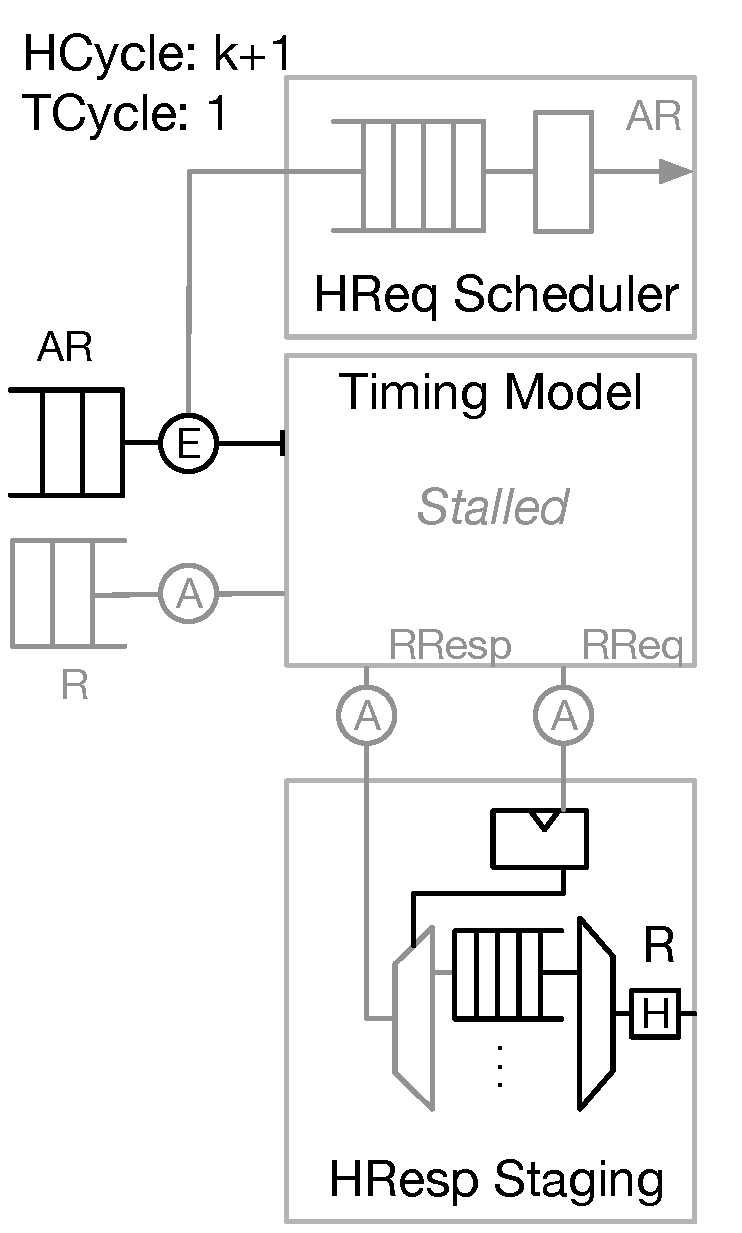
\includegraphics[width=\columnwidth]{figures/model-operation-3.pdf}
        % graffle2pdf -c 3 midas-graphics/graffle/memory-model-operation.graffle figures/model-operation-3.pdf
        \caption{}
        \label{fig:model-operation-3}
    \end{subfigure}
    \begin{subfigure}[t]{0.23\textwidth}
        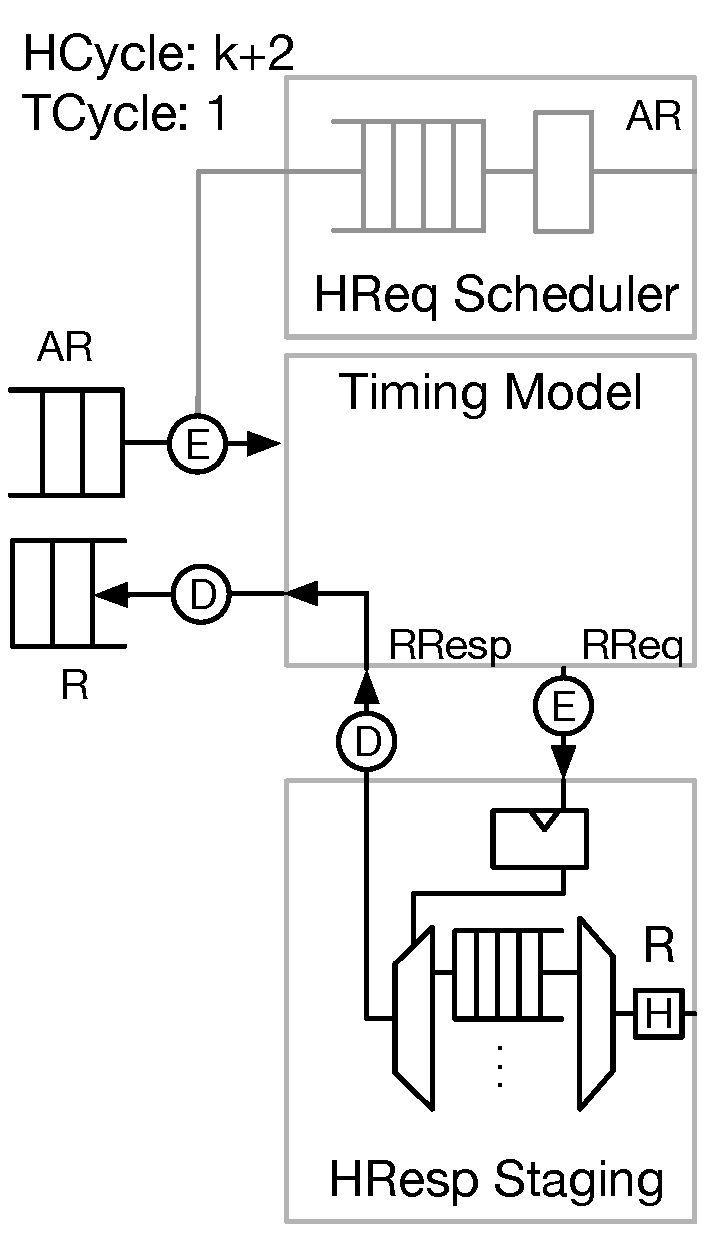
\includegraphics[width=\columnwidth]{figures/model-operation-4.pdf}
        % graffle2pdf -c 4 midas-graphics/graffle/memory-model-operation.graffle figures/model-operation-4.pdf
        \caption{}
        \label{fig:model-operation-4}
    \end{subfigure}
	\centering
    \caption{A \PNAME instance simulating a single-target-cycle read. Data
    tokens carry target transactions~(their target-valid bit is set) whereas
    empty tokens do not carry a target transaction.}
    \label{fig:model-operation}
\end{figure*}


\section{Generator Configuration}\label{sec:generator-parameters}

There are two points at which the model can be configured.  At
\textit{generation time}, the designer selects an instance. At
\textit{simulation time}, the instance is programmed through via simulation
MMIO through its configuration-side interface. Simulation time configurability
permits the designer to perform parameter sweeps without needing to recompile
the simulator bitstream -- at the expense of FPGA resources. Since both timing
and functional components of an instance are provisioned pessimistically,
giving hints to generator can greatly reduce FPGA-resource utilization.

The generator's input configuration consists of a \emph{base} configuration
that is extended with a timing-model configuration. The parameters of the base
configuration are described in the table~\ref{tbl:base-config}. Timing-model
configurations are described section~\ref{sec:timing-model}. Note, ingress and
egress unit generation depends only on parameters of the base configuration.

\begin{table}
\begin{center}
\resizebox{\textwidth}{!}{%
    \begin{tabular}{|p{0.20\textwidth}|p{0.10\textwidth}|p{0.7\textwidth}|}
    \hline
    \textbf{Name} & \textbf{Default} & \textbf{Description} \\
    \hline
    \hline
    \textit{TargetAXIKey} & N/A & Gives the widths of variable width fields in the target-side AXI4 interface. \\
    \hline
    \textit{MaxReads} & N/A & The number of maximum outstanding reads the instance can support.  \\
    \hline
    \textit{MaxWrites} & N/A & As above, but for write transactions. \\
    \hline
    \textit{MaxReadLength} & 256 & The maximum number of beats in a read transaction. (Defaults to AXI4 limit of 256.) \\
    \hline
    \textit{MaxWriteLength} & 256 & As above, but for write transactions. \\
    \hline
    \textit{MaxReadIDs} & $2^{IDWidth}$ & Specifies a bound on the maximum number of AXI4 read channel IDs that will be used by in-flight requests. \\
    \hline
    \textit{MaxWriteIDs} & $2^{IDWidth}$ & As above, but for write transactions. \\
    \hline
\end{tabular}}
\end{center}
\caption{Generator base configuration parameters.}
\label{tbl:base-config}
\end{table}%

\section{Egress Unit Design}\label{sec:egress}

In this section we consider only read responses, as they constitute the bulk of the area of the egress unit.

How the egress unit implements its virtual queues depends on base-generation
parameters (table~\ref{tbl:base-config}), including the maximum number of
requests sharing an ID concurrently,  MaxReadsPerID ($R_{ID,max}$), the maximum
concurrent number of responses across all IDs, MaxReads ($R_{max}$), and the
maximum length, in beats, of a read response, MaxReadLength ($L_{max}$).

The egress unit is provisioned for the worst case, but tries to intelligent
save FPGA resources where possible. To describe the trade off we define virtual
state $VS$ as the total state required to directly implement each virtual
queue:

$$VS = ID_{max}*R_{ID,max}*L_{max}*B$$

Where $B$ are the number of bits per beat. We also define ideal state, $IS$,
the state required to store the maximum number of responses of maximum length.

$$IS = R_{max}*L_{max}*B$$

Note that, if the user does not specify a bound on ($R_{ID,max}$, then, all
responses may share a single ID and thus,

$$VS = IS*ID_{max}$$

The conventional wisdom in design for FPGAs is that BRAM is cheap. Instead of
trying to be clever, for small degrees of virtual state the egress unit
directl implements each of those queues in BRAM, in a structure called a
SRAMMultiFIFO~(SMF)~\cite{LIFPGADesign}. Since the egress unit only ever enqueues into
and dequeues from a single queue, a 1R-1W port BRAM can be used to
co-locate the entries of multiple queues.  Read and write pointers for each
queue are maintained separately in registers. To address a beat, the AXI ID and
the matching read or write pointer are concatenated.

For large virtual state, and when $VS > IS$, directly implementing each virtual
queue in BRAM becomes too expensive. Consider the case in which we assume AXI4
 maximums of 256 unique IDs and 256 beat transactions, a 64-bit data width, and an egress unit provisioned to hold 16 responses. Here, $VS =
8MiB$ but $IS = 32 KiB$.

In this case, the egress uses a level of indirection and dynamically assigns
entries in an SMF, with $R_{max}$ queues of depth $L_{max}$, to responses as
they are received. A translation unit contains a free list and a mapping table,
which for each SMF entry has a valid bit, a head bit, an AXI ID and a next
pointer to an entry holding the next oldest response with the same AXI ID. This
establishes a linked list that maintains an age ordering of responses for the
given AXI channel.

When a response from the host is received, it requests an entry in the SMF from
the translation unit. The granted entry is marked valid, and the next youngest
transaction sharing that AXI ID updates its next pointer.  The response is then
enqueued into the SMF. When the model requests a response, the translation unit
matches on the head of the linked list of the requested AXI ID, returning an
entry index if there is a hit. The response is then dequeued from the SMF
beat-by-beat as the model handshakes on the egress response port.  Once the
final beat has been read from the SMF, the entry is freed, and the next
youngest entry for the AXI ID is marked as the head.

This translation unit is an associative structure that produces an translation
combinationally, and thus tends to be LUT intensive, and may adversely affect
cycle time. To date, our simulations have never been resource constrained, the
critical paths lie in transformed-RTL models, and run with FMR of 1. In the
future, there are many optimizations that could be made to trade host-cycles for
FPGA-resource savings.

Regardless of egress implementation, selecting the right base configuration
parameters can dramatically save resources. Consider the default configuration
of Rocket-Chip, which has an AXI ID width of 4 bits, data width of 64 bits, and
a block size of 64 bytes. Here, a cache refill served in 8 beats -- one eighth
of the AXI4 maximum length -- and can reduce $VS$ from 0.5 MiB to 16
KiB.\footnote{In a Xilinx 7 series architecture, this is 4 36Kb BRAMs ($<$ 1\%
of the BRAM available on the XC7Z045).} Furthermore, in many cases masters do not
issue multiple requests using the same transaction ID to maximize the
flexibility of the slave to reorder requests. Using the same example, and
setting $R_{ID,max}$ to one, sets $VS = IS = 1 KiB$ permitting a direct
implementation to fit in a single BRAM of any modern FPGA architecture.

Presently, the generator uses a direct implementation if $VS <= 32 KiB$ or $VS
= IS$. We leave defining a better heuristic to future work. Ultimately, how
handwritten-RTL models should be optimized is a system-level question that
depends on the resource utilization the project, desired FMR, and
the host-FPGA architecture. Indeed, simulators under BRAM pressure may wish to use
translation logic when the generator by default may choose otherwise. At time
of writing, MIDAS generated simulators tend to be under LUT pressure. In this
case, even when $VS > IS$, directly implementing the virtual queues may be
desired.

\section{Generic Timing-Model Classes}

We provide two classes of \emph{generic} timing-models: a latency-bandwidth
pipe and a bank-conflict model. These can be used to abstractly model DRAM or
any other large AXI4 memory-slave device that may be backed by a different
memory technology.

\subsection{Latency-Bandwidth Pipe}

The latency-bandwidth pipe timing-model class applies independently
programmable latencies to read and write requests. It does not accept any new
requests beyond a programmable limit; this serves as a coarse-grain bandwidth
bound via Little's law. Note, for systems that make requests of varying
lengths, the simulated memory bandwidth will be reduced when making shorter
requests. This model never reorders target requests.

\noindent Runtime parameters are shown in table~\ref{tbl:lbp-programmable-registers}.

\begin{table}
\begin{center}
\resizebox{\textwidth}{!}{%
    \begin{tabular}{|p{0.20\textwidth}|p{0.8\textwidth}|}
    \hline
    \textbf{Name} & \textbf{Description} \\
    \hline
    \hline
    \textit{ReadMaxRequests} & Sets the maximum number of in-flight read
        requests the timing-model will accept, before apply backpressure to
        request channels. \\
    \hline
    \textit{WriteMaxRequests} & As above, but for write requests. \\
    \hline
    \textit{ReadLatency} & Sets the latency of a read-request. \\
    \hline
    \textit{WriteLatency} & As above, but for write transactions. Note, this length
        is measured from the cycle at which both write address and write data
        requests have been completed to the cycle at which the write
        acknowledgment is first produced. \\
    \hline
\end{tabular}}
\end{center}
\caption{Programmable registers of the latency-bandwidth pipe.}
\label{tbl:lbp-programmable-registers}
\end{table}%

\clearpage
\subsection{Bank-Conflict Model}\label{sec:bank-conflict}

The bank-conflict timing-model class adds a penalty of $max(0, t_{CP} - t_{\Delta})$ to a
base latency if a read or write request used the bank $t_{\Delta}$ cycles
prior, where $t_{CP}$ is the maximum conflict penalty. The model has a
reconfigurable number of banks and bank address assignment.  The bank address
is assigned by setting an offset and a mask, where: $$Address_{Bank} =
(Address_{Physical} >> Offset) \& Mask$$  The timing-model must be provisioned
with the maximum number of banks at generation time. This model may reorder requests.

\noindent Generation and runtime parameters are shown in
tables~\ref{tbl:bc-generator-parameters}
and~\ref{tbl:bc-programmable-registers} respectively.

\begin{table}[htb]
\begin{center}
\resizebox{\textwidth}{!}{%
    \begin{tabular}{|p{0.20\textwidth}|p{0.10\textwidth}|p{0.7\textwidth}|}
    \hline
    \textbf{Name} & \textbf{Default} & \textbf{Description} \\
    \hline
    \hline
    \textit{MaxBanks} & N/A & Specifies the maximum number of banks the timing-model can support. Must be a power of 2. \\
    \hline
    \textit{MaxLatencyBits} & 12 & Defines the number of bits used in cycle accountings of target-time. \\
    \hline
\end{tabular}}
\end{center}
\caption{Additional generation parameters of the bank conflict timing-model.}
\label{tbl:bc-generator-parameters}
\end{table}%

\begin{table}[htb]
\begin{center}
\resizebox{\textwidth}{!}{%
    \begin{tabular}{|p{0.20\textwidth}|p{0.8\textwidth}|}
    \hline
    \textbf{Name} & \textbf{Description} \\
    \hline
    \hline
    \textit{ReadMaxRequests} & Same as latency-bandwidth pipe (table~\ref{tbl:lbp-programmable-registers}) \\
    \hline
    \textit{WriteMaxRequests} & Same as latency-bandwidth pipe (table~\ref{tbl:lbp-programmable-registers}) \\
    \hline
    \textit{Latency} & Sets the base latency of a read or write transaction. \\
    \hline
    \textit{ConflictPenalty} & Sets the maximum number of additional cycles a
        conflicting transaction will be delayed. \\
    \hline
    \textit{BankAddrOffset} & Specifies the position of the LSB of the bank
        address within the physical address.  \\
    \hline
    \textit{BankAddrMask} & Specifies the mask used to extract the bank address from the physical address. \\
    \hline
\end{tabular}}
\end{center}
\caption{Programmable registers of the bank conflict timing-model.}
\label{tbl:bc-programmable-registers}
\end{table}%

\clearpage
\section{DDR3 Timing-Model Classes}

We provide two DDR3 timing-model classes based around the
FCFS~(section~\ref{sec:fcfs}) and FR-FCFS~(section~\ref{sec:frfcfs}) MAS. Both
timing-model classes can be decomposed into three stages: transaction
scheduler, MAS, and response buffer.

The transaction scheduler consists of a single unified transaction queue that
can enqueue both a AXI4 read and write transaction in a single cycle, with reads
given priority when only one slot is available. Transactions are passed to the
MAS as they can be accepted, at a rate of one transaction per cycle.  Different
transaction scheduling schemes are left to future work.

The MAS contains a set state-tracking modules for every rank and bank; these
modules indicate what commands that rank or bank may legally accept on a given
cycle. Each MAS has data structures for the memory references it may schedule
across; these structures add additional metadata to the transcation to ease
scheduling decisions. On every target-cycle, the MAS selects a legal command
based on the available references. The selected command is broadcasted back to
each of the bank and rank-state trackers.  Both MAS use a preemptive all-ranks
refresh scheme, that makes no attempt to pull-in or delay refresh commands.
When a refresh is required, commands for pending references are not considered:
the MAS precharges every open bank in every rank, and issues REF commands as
soon as it may legally do so.

Both timing-model classes will attempt to return a read response a single cycle
after they would receive the first beat from DRAM. Write acknowledgements are
returned the cycle after a CASW command is issued. However, in the event that
the target is not ready to accept responses, completed transactions are stored
in seperate read and write response buffers, with capacities large enough to
hold the maximum number of outstanding requests the model may accept.

Presently, models assume the width of the DRAM-system bus is one half of the width of the
target-AXI4 interface. No explicit device width is passed to the timing
model: choice of device width trickles down into other configuration
parameters. For example, for a given memory system capacity, using x4 devices
over x8 devices reduces per-device density~(reducing $t_{FAW}$,
$t_{RRD}$, and $t_{RFC}$) and increases DRAM-page size, which may change the
address mapping for certains types of MAS.  However, it takes twice as many
devices to fill the same system-bus width, which makes it more difficult to
build high-performance multi-rank memory systems.

As a final note, these models may be used to model DDR2 and DDR4 memory systems with an
appropriate choice of timing parameters, however they have only been validated
against DDR3 models at time of writing.

\subsection{Common Generation and Runtime Parameters}

Each model shares generation-time configurations that describe the
the memory organization, including the number of ranks,
banks per rank, and rows per bank. The models accept all of the DRAM timings supported by DRAMSim2~(described in
section \ref{sec:dram-arch}, table \ref{tbl:dram-timings}, with the exception
of $t_{XP}$ and $t_{CKE}$, as runtime parameters.

\noindent Generation and runtime parameters are shown in
tables~\ref{tbl:common-MAS-generator-parameters}
and~\ref{tbl:common-MAS-programmable-registers}
respectively.

\begin{table}[htb]
\begin{center}
\resizebox{\textwidth}{!}{%
    \begin{tabular}{|p{0.20\textwidth}|p{0.10\textwidth}|p{0.7\textwidth}|}
    \hline
    \textbf{Name} & \textbf{Default} & \textbf{Description} \\
    \hline
    \textit{MaxRanks} & N/A & The maximum number of ranks. Must be a power of two. \\
    \hline
    \textit{MaxBanks} & N/A & The maximum number of banks \emph{per rank}. Must be a power of two.  \\
    \hline
        \textit{MaxRows} & N/A & The maximum number of rows \emph{per bank}. Must be a power of two.\\
    \hline
\end{tabular}}
\end{center}
\caption{Common generation parameters of the DDR3 MAS models.}
\label{tbl:common-MAS-generator-parameters}
\end{table}%

\begin{table}[htb]
\begin{center}
\resizebox{\textwidth}{!}{%
    \begin{tabular}{|p{0.25\textwidth}|p{0.75\textwidth}|}
    \hline
    \textbf{Name} & \textbf{Description} \\
    \hline
    \textbf{DRAM Timings} & See table~\ref{tbl:dram-timings}. \\
    \hline
    \textit{ReadMaxRequests} & Same as latency-bandwidth pipe (table~\ref{tbl:lbp-programmable-registers}) \\
    \hline
    \textit{WriteMaxRequests} & Same as latency-bandwidth pipe (table~\ref{tbl:lbp-programmable-registers}) \\
    \hline
    \textit{BankAddrOffset} & Same as bank-conflict model (table~\ref{tbl:bc-programmable-registers}) \\
    \hline
    \textit{BankAddrMask} & Same as bank-conflict model (table~\ref{tbl:bc-programmable-registers}) \\
    \hline
    \textit{RankAddrOffset} & Same mechanism as above for defining rank address assignment. \\
    \hline
    \textit{RankAddrMask} & Same as bank-conflict model (table~\ref{tbl:bc-programmable-registers}) \\
    \hline
    \textit{RowAddrOffset} & Same mechanism as above for defining row address assignment. \\
    \hline
    \textit{RowAddrMask} & See above. \\
    \hline
\end{tabular}}
\end{center}
\caption{Common programmable registers of the DDR3 MAS models.}
\label{tbl:common-MAS-programmable-registers}
\end{table}%
\clearpage

\subsection{FCFS MAS Model}

This class models a FCFS MAS (see section~\ref{sec:fcfs}) with
programmable open and closed page policies. This model considers the head of
the transaction queue and the most recently completed reference to generate
candidate commands.  The close-page policy always issues auto-precharge CAS
commands, which close the row without requiring an expicity precharge command,
even if the next reference accesses the same row.  True to its name, this model
never reorders target requests.

\noindent Additional runtime parameters of this timing model class are shown in
table~\ref{tbl:fcfs-programmable-registers}.

\begin{table}[htb]
\begin{center}
\resizebox{\textwidth}{!}{%
    \begin{tabular}{|p{0.20\textwidth}|p{0.8\textwidth}|}
    \hline
    \textbf{Name} & \textbf{Description} \\
    \hline
    \hline
    \textit{OpenPagePolicy} & When set, the model does not close an open row immediately after each request. \\
    \hline
\end{tabular}}
\end{center}
\caption{Programmable registers of the FCFS MAS model.}
\label{tbl:fcfs-programmable-registers}
\end{table}%

\subsection{FR-FCFS MAS} This class models a FR-FCFS MAS
(section~\ref{sec:frfcfs}) with an open or closed-page policy. The MAS considers
references to all banks and ranks simultaenously; all references are stored in
a single collapsing buffer, with additional bits to track if they are
ready~(\emph{isReady}, they hit an open row buffer), and whether PRE
commands for the request may be considered~(\emph{mayPRE}, there are no other
ready references that address the same bank). CAS, ACT, and PRE arbiters select
the oldest legal command of that type from the legal candidates, and are
scheduled in descending priority (CAS before ACT before PRE).

This model reorders target requests.

The generation and runtime parameters as the FR-FCFS MAS model are shown
in table~\ref{tbl:frfcfs-generator-parameters}.

\begin{table}[htb]
\begin{center}
\resizebox{\textwidth}{!}{%
    \begin{tabular}{|p{0.20\textwidth}|p{0.10\textwidth}|p{0.7\textwidth}|}
    \hline
    \textbf{Name} & \textbf{Default} & \textbf{Description} \\
    \hline
    \textit{RefQueueDepth} & 16 & The maximum number references that MAS can
        accept in its collapsing buffer. \\
    \hline
\end{tabular}}
\end{center}
\caption{Generation parameters of the FR-FCFS MAS model.}
\label{tbl:frfcfs-generator-parameters}
\end{table}%

\subsection{Instrumentation \& Power Modeling}

By default, both MAS timing-models include instrumentation to measure
microarchitectural events required by Micron's power-estimation spreadsheet.
This includes counters for: the number of cycles each rank spends with all
banks precharged, and the number of ACTs, CASW, and CASR commands issued to
each rank. By sampling these counters periodically, time-series plots of DRAM
power dissipation can be generated.

\subsection{Comparison to DRAMsim2}

Perhaps the most frequent question we receive about the model is how it
compares to DRAMsim2: we enumerate some noteworthy differences here.

\begin{enumerate}
    \item \textbf{Different controller modeling decisions.} Even with the same
        DRAM timings and memory organization, model instances and
        DRAMSim2 exhibit different per-transaction latencies. Commands for a
        new transaction may be issued one and two cycles~(FCFS and FR-FCFS MAS
        respectively) after the request was received, versus three cycles in
        DRAMsim2. DRAMsim2 releases a response once all beats have been
        received -- adding an additional three cycle latency to read-response
        in the case of an 8 beat burst. Finally, the MAS implementations differ
        slightly and thus produce command schedules for the same transaction
        trace. This introduces some variability in the latencies seen by each
        request.\footnote{MAS implementations, even of well-described
        algorithms, vary across software simulators too, as shown
        in~\cite{ramulator}.}

    \item \textbf{No multi-channel support.} While software DRAM simulators
        support multi-channel configurations, in MIDAS we expect the user will
        use separate model instances for each channel, just as there would be
        multiple physical controllers in an implementation.

    \item \textbf{No modeling of power-down or self-refresh modes.} Will be
        added alongside power modeling support.

\end{enumerate}

\section{Validation}

Validation of the memory timing model was done in RTL simulation. Here, model
instances are generated and simulated in isolation with a memory-reference trace.
A CPP test harness binds to each of its interfaces.  The host-side interface
connects to a C++ memory model derived from that used in Rocket-Chip. The host
memory can be configured to be a single-cycle memory system, or a particular
configuration of DRAMSim2.  The configuration-side interface is bound to a
simple AXI4 driver that programs the instance based on command-line arguments
passed to the simulator, spoofing the initialization that would occur at the
start of a MIDAS simulation. The driver of the target-side interface accepts a
memory-reference trace from which it generates simulation tokens to drive the instance.
Memory-reference traces consist of address, data, either the write data or the
expected read-response data, and target-cycle, the earliest cycle at which the
request should be made visible to the instance. Output tokens from the instance are
collected, and the timing data for each transaction is dumped to a file for
post-processing. This includes the target- and host-cycles at which a request is
first accepted and a response is first presented for each memory reference.

We used different approaches for validating the generic timing-model classes
and the DRAM timing-model classes. For the prior, the per-transaction latencies
can be determined easily a priori for a given memory-reference trace\footnote{This
includes a model of the backpressure the master presents to the AXI4 read and
write response channels, as head-of-line blocking due to backpressure on
responses will further delay younger responses.  In our validation flow, we
ensure the master is always ready to accept a new response.} Thus, we validate
instances by comparing the timing dumps against those produced by a golden model
for each memory-reference trace. The timings must match or the instance fails
validation.

Validating DRAM timing-model classes is fundamentally more difficult as there
is no complete specification against which to compare transaction timings.
One could use DRAMsim2 as that specification, but this requires that the
timing-model instances abide by all of the same modeling decisions made by
DRAMsim2~(some of which are arbitrary). Indeed, different software models like
Ramulator and USIMM exhibit different behaviors than DRAMSim2 even when
configured to model indentical memory systems~\cite{ramulator}. Alternatively,
writing a software golden-model would be tantamount to writing another
cycle-accurate DRAM-simulator like DRAMsim2.

Instead, we use same approach employed by software simulators. In
addition to dumping transaction timing information, DRAM-timing model classes
also dump a DRAM-command schedule. This drives a RTL golden model of a
single-device slice of the memory organization which detects DRAM timing
violations. DDR2, DDR3, and DDR4 golden models and example testbenches are
freely provided by Micron\cite{microngolden}. We validated against DDR3, making small
modifications to the provided example testbench to support validation of
multi-rank organizations and to accept the generated command trace.

Unfortunately, this approach does not prove the model faithly models the MAS it
purports to model, as there are still infinitely many legal schedulings of DRAM
commands for a given memory-reference trace. To sanity check against this,
Ramulator passes the same memory-reference trace to a collection of other
software simulators including DRAMsim2 and USIMM and compares
target-runtime~(average bandwidth).

Augmenting this approach, our validation flow generates plots that can be used
to further inspect deviations between the models. This includes latency
histograms, and rolling averages of achieved DRAM-bandwidth over time.


\chapter{Methodology}
\section{Target Design Configuration}

To demonstrate of the use of our generator, we evaluated two
microarchitecturally different processors:  Rocket, a 5-stage single-issue
in-order core, and BOOM, a superscalar out-of-order core~\cite{boom}. Both
microarchitectures leverage the open-source Rocket-Chip SoC
generator~\cite{rocketchip}. As described in section~\ref{sec:targetandhostmachines}, all of the instances of RocketChip used in
this report have same top-level I/O and are modeled as part of a target with
the MIDAS SDF network shown in figure~\ref{fig:default-target}.

Both cores implement the 64-bit scalar RISC-V ISA~\cite{Waterman:EECS-2016-118,
Waterman:EECS-2016-161}\footnote{User level specification v2.1, privileged
specification v1.9} which includes support for atomics, IEEE 754-2008
floating-point, and page-based virtual memory (RV64IMAFD).
Table~\ref{tbl:target} lists the selected configurations of the target
processors.\footnote{Note that BOOM-2w roughly approximates the configuration
of the ARM Cortex-A9 processor, which coincidentally is same microarchitecture
embedded in the Zynq host.}. Unfortunately, neither configuration includes an
L2 cache as it was  temporarily removed in the version of RocketChip used to
conduct the evaluation. As a final note, the Rocket configuration we used
includes a non-blocking data cache (instead of the default blocking
implementation). Unlike a classic RISC pipeline, Rocket's backend includes a
scoreboard that allows it to make multiple memory requests when there are no
intermediate dependent instructions.

\begin{table}
\begin{center}
\resizebox{0.6\textwidth}{!}{%
\begin{tabular}{|r|c c|}
    \hline
     & \textbf{Rocket} & \textbf{BOOM-2w} \\
    \hline
    \textit{Fetch-width} & 1 & 2 \\
    \textit{Issue-width} & 1 & 3 \\
    \textit{Issue slots} & - & 16 \\
    \textit{ROB size} & - & 48 \\
    \textit{Ld/St entries} & - & 16/16 \\
    \textit{Physical registers} & 32(int)/32(fp) & 110 \\
    \textit{Branch predictor} & - & tage \\
    \textit{MSHR entries} & 2 & 6 \\
    \textit{L1 I\$ and D\$} & \multicolumn{2}{c|}{16KiB / 16KiB} \\
    \textit{ITLB and DTLB reaches} & \multicolumn{2}{c|}{128KiB / 128KiB} \\
    \hline
\end{tabular}}
\end{center}
\caption{Processor Parameters}
\label{tbl:target}
\end{table}%

%\begin{table*}
%\centering
%	\begin{tabular}{|c|S[table-format=5]|c|S[table-format=5]|c|S[table-format=5]|c|S[table-format=5]|c|}
%	\hline
%	& \multicolumn{2}{c|}{\textbf{Latency-Bandwidth Pipe}} & \multicolumn{2}{c|}{\textbf{Bank Conflict Model}} & \multicolumn{2}{c|}{\textbf{FIFO MAS}} & \multicolumn{2}{c|}{\textbf{FR-FCFS}} \\
%	\hline
%	\textbf{Resource} & \textbf{Utilization} & \textbf{\%} & \textbf{Utilization} & \textbf{\%} & \textbf{Utilization} & \textbf{\%} & \textbf{Utilization} & \textbf{\%} \\
%	\hline
%	\textit{LUT} & 3586 & 1.6 & 4170 & 1.9 & 3812 & 1.7 & 6822 & 3.1 \\
%	\textit{LUTRAM} & 651 & 0.9 & 607 & 0.8 & 655 & 0.9 & 693 & 1.0 \\
%	\textit{FF} & 3146 & 0.7 & 3929 & 0.9 & 3426 & 0.8 & 5282 & 1.2 \\
%	\textit{BRAM} & 11 & 2.0 & 11 & 2.0 & 11 & 2.0 & 11 & 2.0 \\
%	\hline
%	\end{tabular}
%
%\caption{Resource utilization of various memory system models for Xilinx zc706 FPGA}
%\label{tbl:utilization}
%\end{table*}

\section{System Software}

Unless otherwise stated, all benchmarks were run on Linux (kernel version
4.6.2). Unfortunately, at time of writing we do not have the ability to proxy a
block device requests over the tether (as is done with I/O). Thus for each
workload, we built a minimal BusyBox image and included all required files for
that workload within the image's initramfs.  Generally, workloads were compiled
statically (using \texttt{gcc -02}). When required, namely for the Java workloads, we
built library dependencies using the Yocto (\texttt{riscv-poky}) Linux
distribution generator. After packaging up the complete linux image, it is
built into an instance of the Berkeley Bootloader (BBL).

Despite our best efforts, this process produces relatively large BBL instances
($>$ 10MiB), which are slow to load directly over the tether.  We modified
\texttt{riscv-fesvr} to permit the MIDAS master to detect and accelerate program load
out-of-band (instead of fully simulating the process over the tether).

Finally, present limitations regarding how console I/O is proxied to
\texttt{riscv-fesvr} can dramatically slow down simulation depending on the
volume of target console I/O. \footnote{Changes introduced to
\texttt{riscv-fesvr} with the priviledge specification 1.10 updates remove this
bottleneck, as the host is no longer is required to acknowledge console
output.} To circumvent this, all console output is piped to a file on the
target's filesystem. At the end of the workload, the file is dumped to the
console, and \texttt{riscv-fesvr} enters a custom fast I/O mode.  Thus, low FMR
is maintained without pertubing program execution. In our evaluation flow, no
console input is ever presented to the target; the \texttt{init} script of the
linux image includes all of the commands required to run and measure the
desired workload, afterwhich it powers down the machine (See listing~\ref{lst:init} for an example).\\

\lstdefinestyle{init}{
    frame=lines,
    captionpos=b,
    %xleftmargin=\parindent,
    language=bash,
    showstringspaces=false,
    basicstyle=\footnotesize\ttfamily,
    %keywordstyle=\bfseries\color{green!40!black},
    commentstyle=\itshape\color{blue},
    identifierstyle=\color{black},
    stringstyle=\color{orange},
}

\lstset{style=init}

\begin{lstlisting}[caption={An example init script generated during the build process},label={lst:init}]
    cd /biancolin
    # Periodically polls HPM counters to measure target events
    /biancolin/rv_counters/rv_counters >> dump &
    sleep 1

    # Run the workload
    ./hello >> dump 2>&1

    # Cleanup, kill the counter program, and cat results to console
    killall rv_counters
    while pgrep rv_counters > /dev/null; do sleep 2; done
    sync
    cat dump
    poweroff -f
\end{lstlisting}

\section{Measuring the Target}

Measurements of the target design occur in two places.
Memory timing-model instances collect their own statistics, and
as described previously, are read with MMIO through the simulation
interconnect. While these measurements can be made while the simulation is
executing, in our evaluation we halt target execution to get a consistent
snapshot. Regardless, these measurements do not perturb simulation behavior.

While we ultimately plan to support transformations that permit
measuring generated-RTL models non-invasively, in this report,
measurements of the core are made using a process running on the target machine,
\texttt{rv\_counters}. This program wakes up every hundred million target
cycles to read the core's hardware performance monitor (HPM) which by default measures
cycles and instructions retired. Additionally, the HPM provides 29 other counters to measure
events defined by the microarchitect like branch mispredictions or data
cache misses (see~\cite{Waterman:EECS-2016-161} section 3.1.15).
\texttt{rv\_counters} prints the values of these counters to standard out; they are collected
in a second file in the target filesystem. Since polling events are both
short-lived and infrequent, perturbations in target execution are insignificant.

When a specific event was not measured by the existing design, we added them
manually to Rocket-Chip. In addition to measuring conventional
microarchitectural events, with this mechanism we were also able to measure the
execution time of regions of the application, like memory allocations in the
JVM, with effectively zero pertubation. To do this, we instrumented the target
program with specialy encoded NOP instructions which would enable and disable
an incrementer when decoded.

\section{Workloads}

To demonstrate that our platform allows us to perform high-fidelity experiments
involving realistic software applications without sub-sampling execution, we
chose two non-trivial benchmark suites, the SPEC 2006 CPU
benchmarks~\cite{spec_cpu_2006} and the DaCapo benchmarks~\cite{dacapo}.

\subsection{SPECint2006 Benchmarks} The SPECint2006 benchmarks are defacto
standard to benchmarking sequential performance of general-purpose
microprocessors, and widely used by industrial computer architects to validate
their designs. Academic computer architects seldom run the complete
``reference" workload due to their length which commit between 23-25 trillion
dynamic instructions in RISC-V (RV64G).

Table~\ref{tbl:spec} shows the dynamic instruction counts and the cache and TLB
misses per 1000 instructions~(MPKI) for each benchmark executed with its test
inputs. It would take at least 8 days to run the test workloads on a single
instance of a very fast microarchitectural cycle-accurate software simulator
(400~KIPS)~\cite{marssx86}, and nearly two years to run the reference
workloads. For comparison, a single MIDAS simulator, assuming ($f_{fpga} = 40
MHz, FMR = 1.25, CPI_{target} = 2)$ takes approximately 5 hours and 17 days to
run test and reference workloads respectively.

\begin{table}[t]
	\begin{center}
    \resizebox{0.6\textwidth}{!}{
        \begin{tabular}{|c|S[table-format=3.1]|S[table-format=3.1]|}
        \hline
        \textbf{Benchmarks} & \textbf{Instructions~(B)} & \textbf{MPKI} \\
        \hline
		\textit{400.perlbench} & 2.6 & 49.5 \\
		\textit{401.bzip2} & 34.4 & 27.5 \\
		\textit{403.gcc} & 5.4 & 37.2 \\
		\textit{429.mcf} & 3.5 & 274.6\\
		\textit{445.gobmk} & 66.4 & 36.4 \\
		\textit{456.hmmer} & 16.5 & 4.3 \\
		\textit{458.sjeng} & 18.9 & 23.1 \\
		\textit{462.libquantum} & 0.3 & 32.0 \\
		\textit{464.h264ref} & 104.2 & 7.5 \\
		\textit{471.omnetpp} & 1.9 & 61.0 \\
		\textit{473.astar} & 22.8 & 45.8 \\
		\textit{483.xalancbmk} & 0.4 & 64.3 \\ 
		\hline
		\end{tabular}
		\label{tbl:spec_test}
    }%
	\caption{Dynamic instruction counts and MPKI for the SPECint2006 benchmarks with test inputs}
    \vspace{0.2cm}

    \resizebox{0.6\textwidth}{!}{%
        \begin{tabular}{|c|S[table-format=3.1]|S[table-format=3.1]|}
        \hline
        \textbf{Benchmarks} & \textbf{Instructions~(B)} & \textbf{MPKI} \\
        \hline
		\textit{403.gcc} & 1366.5 & 54.2 \\
		\hline
		\end{tabular}
    }%
	\end{center}
    \caption{Dynamic instruction count and MPKI for SPECint2006 gcc with its reference input (all workloads)}
	\label{tbl:spec}
\end{table}

\subsection{DaCapo Benchmarks}

\begin{table}
\begin{center}
\resizebox{0.6\textwidth}{!}{%
	\begin{tabular}{|c|S[table-format=3.1]|S[table-format=3.1]|}
	\hline
	\textbf{Benchmarks} & \textbf{Instructions~(B)} & \textbf{MPKI} \\
	\hline
	\textit{avrora} & 216.5 & 51.2 \\
	\textit{luindex} & 72.5 & 30.5 \\
	\textit{lusearch} & 131.5 & 34.1 \\
	\textit{pmd} & 109.6 & 34.1 \\
	\textit{sunflow} & 124.5 & 41.6 \\
	\textit{xalan} & 152.9 & 37.9 \\
	\hline
	\end{tabular}
}%
\end{center}
\caption{Dynamic instruction counts and MPKI for the DaCapo benchmarks with the ``small'' input size}
\label{tbl:dacapo}
\end{table}

The DaCapo benchmarks are widely used Java benchmarks that represent full Java
applications, including the Lucene search engine and a raytracer. We use
version 9.12 of the benchmark suite and exclude the benchmarks that do not run
on recent versions of JikesRVM. Specifically, we run \emph{avrora},
\emph{luindex}, \emph{lusearch}, \emph{pmd}, \emph{sunflow} and \emph{xalan}.

For each benchmark, we ran one full pass of the ``small'' input size,
accounting for both class loading and Just-in-Time compilation. We believe that
this gives a comprehensive and realistic view of the full execution of a Java
program. Figure~\ref{tbl:dacapo} shows the dynamic instruction counts and MPKI
for each benchmark with the ``small'' input size.

JikesRVM is configured to use the \emph{MarkSweep} garbage collector and the
default settings. MarkSweep is a non-relocating Mark \& Sweep Garbage Collector
with a segregated free-list allocator (meaning that it maintains a number of
free lists for different size classes of objects, with a shared pool of pages
that can be acquired and released by these free lists).


%\chapter{Validation}
%Validating timing-models, especially those that may not have a strict
specification, is a fundamentally difficult proposition. Models like Ramulator
and DRAMsim2 can claim a strong degree of validation checking their generated
command stream with an RTL golden model that detects DRAM timing violations.
Since our DRAM models do not model refresh, we cannot re-use this strategy.
Lacking a "golden" specification against which to validate our models, we
employ three strategies to check our models:

\begin{enumerate}
    \item \textbf{Validation against a manually-written C++ model.} The C++ model forms a
        specification against which the instance is checked. Here, we drive both the
        C++ model and an RTL simulation of the instance with the same memory
        traces and compare the cycle-by-cycle behavior.

    \item \textbf{Sanity checking against DRAMSim2.} Here, we replace the C++
        model with a reference model (DRAMSim2). As before, we present
        identical memory traces to the reference and instance and compare
        the cycle-by-cycle behavior, and assess the degree to which they differ.

    \item \textbf{Sanity checking at the system-level.} In FPGA simulation, we run
        micro-benchmarks on the target whose memory-system behavior can be
        deduced \textit{a priori}.
\end{enumerate}

\begin{figure}[t]
	\centering
	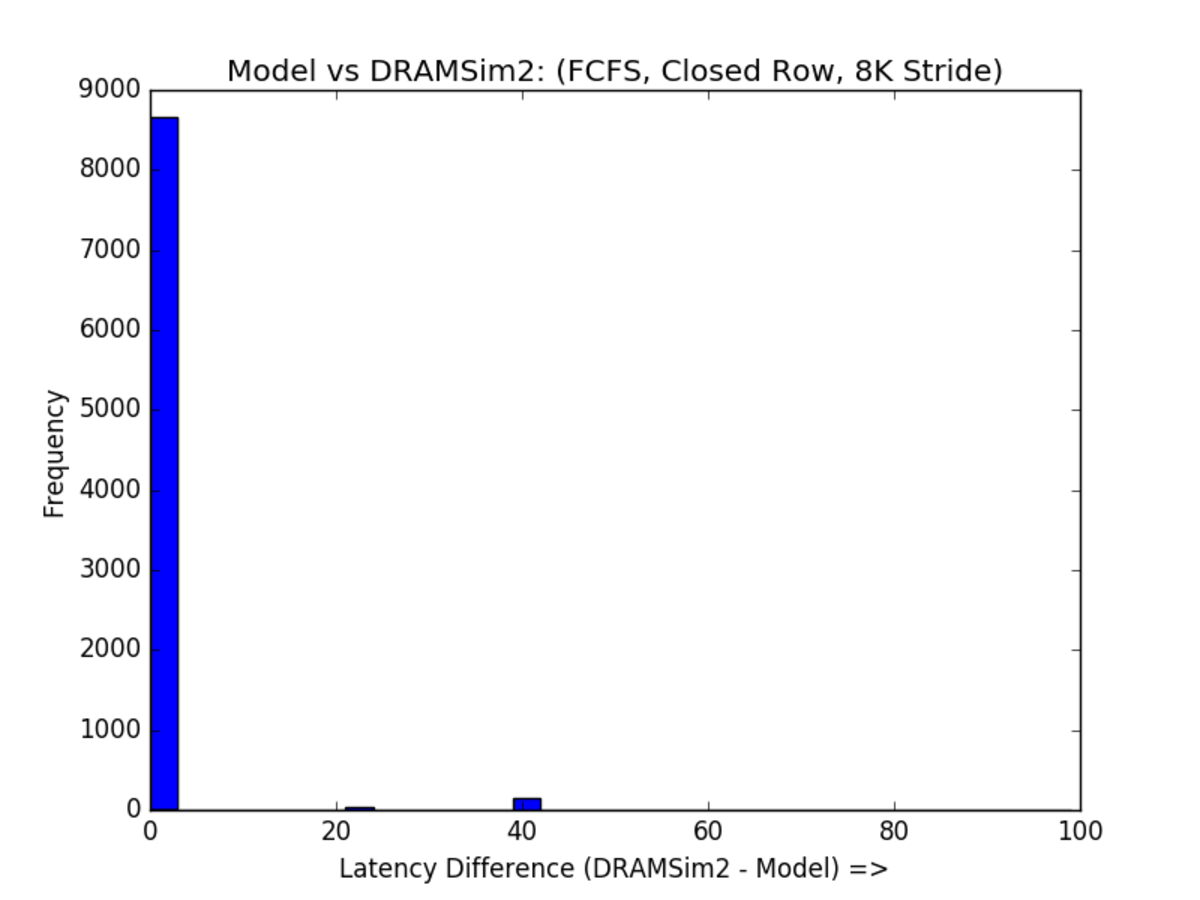
\includegraphics[width=0.75\columnwidth]{figures/close_row_stride.pdf}
    \caption{Histogram of latency-differences between our FCFS MAS model and DRAMSim2 (8 Banks, 8K pages, 9:1 read:write ratio,  $T_{RP},T_{CS},T_{RCD} =
    10$). Timing abberations are due to refresh.}
  \label{fig:error_histogram}
\end{figure}

While these techniques are sufficient to show that the models capture important
trends when sweeping a configuration setting, future work could explore a closer
comparison of our model against a cycle-accurate model like DRAMSim2.

Figure~\ref{fig:error_histogram}, illustrates the effect of refresh even when
the model is being driven lightly (periodic requests every 50 cycles) in trace
driven mode. We intend to employ more exhaustive validation against these
simulators as additional features are added to our models.



%\chapter{Evaluation}
%In this section, we validate the behaviors of our DRAM timing models with
the SPECint2006 benchmarks whose characteristics are well known for computer architects.

\subsection{Latency Configurations}

% \begin{figure*}
% \begin{subfigure}[t]{0.33\textwidth}
% 	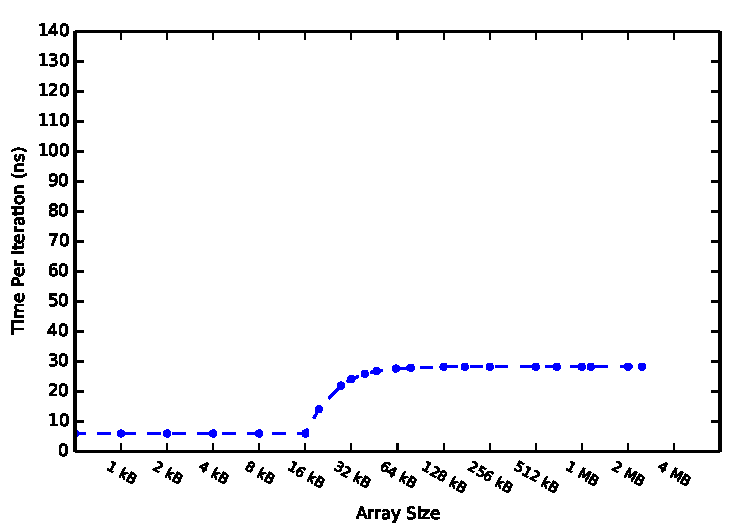
\includegraphics[width=\textwidth]{figures/ccbench_lat1.pdf}
% 	\caption{DRAM Latency = 1}
% \end{subfigure}
% \begin{subfigure}[t]{0.33\textwidth}
% 	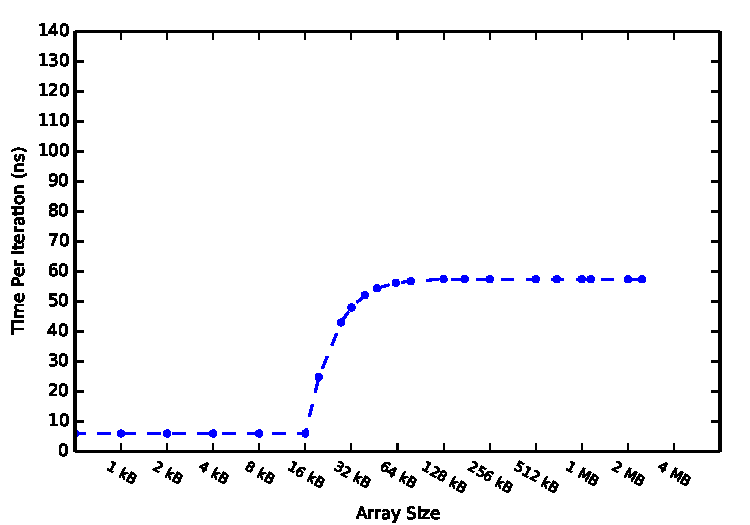
\includegraphics[width=\textwidth]{figures/ccbench_lat30.pdf}
% 	\caption{DRAM Latency = 30}
% \end{subfigure}
% \begin{subfigure}[t]{0.33\textwidth}
% 	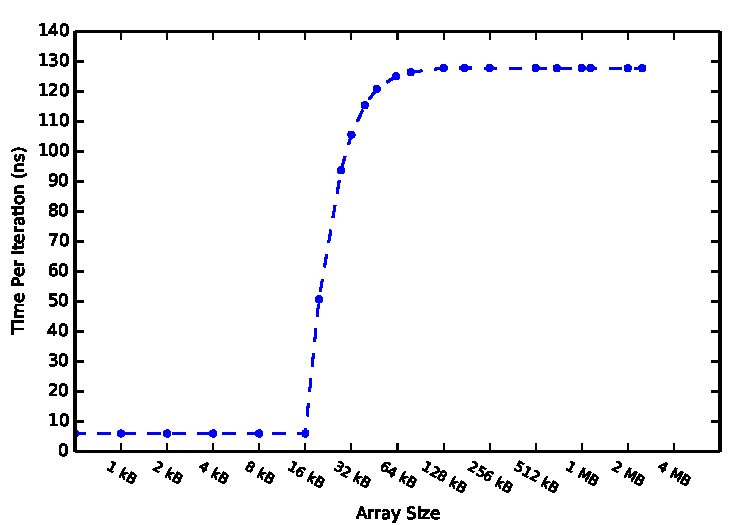
\includegraphics[width=\textwidth]{figures/ccbench_lat100.pdf}
% 	\caption{DRAM Latency = 100}
% \end{subfigure}
% \caption{Latency Validation}
% \label{fig:lat_val}
% \end{figure*}

% Figure~\ref{fig:lat_val} shows the results of cache hierarchy tests in \textit{ccbench}
% for BOOM-2w, assuming its frequency is 1GHz. We can see that the amount of
% the time per iteration with arrays bigger than the cache size observed by the target system
% increases by the delay of the off-chip memory as the DRAM latency increases.
% In this case, 1 cycle is 1ns, and thus, the time per iteration with large arrays
% increases by 30ns and 100ns as the DRAM latency increases by 30 cycles and 100 cycles,
% respectively.

Figure~\ref{fig:gcc_ref} shows how CPI varies over time for \textit{403.gcc} with the reference
input set running on the Rocket processor. We first measure the performance with a
magic memory with a one-cycle latency to determine the maximum performance the Rocket processor can
achieve. Next, we increase the memory latency to 30 cycles and see how much the Rocket processor
slows down.

This experiment demonstrates that our simulation methodology enables ``what-if'' experiments
regarding memory parameter configurations for very long-running applications, which is
practically impossible with software simulators. Note that the dynamic instruction count for
\textit{403.gcc} with the reference input is 1.3 trillion (Table~\ref{tbl:spec_ref}). The
effective simulation rate is 29 MHz on the FPGA, whose operating frequency is 40 MHz. The
simulation slow-down is due to the communication overhead between the software components and the
FPGA-based simulator.

\begin{figure*}
	\centering
	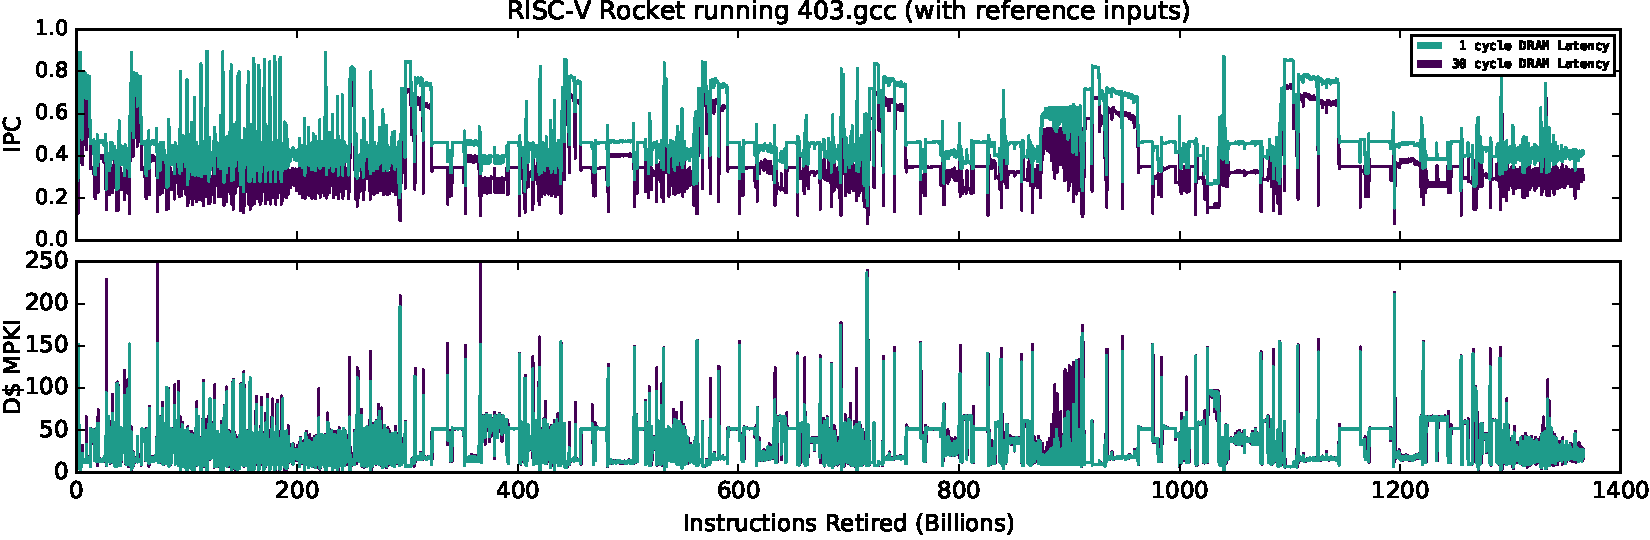
\includegraphics[width=0.95\textwidth]{figures/403-gcc-ref.pdf}
	\caption{CPI and D\$ MPKI for 403.gcc with the reference input running on the Rocket processor}
	\label{fig:gcc_ref}
\end{figure*}

\subsection{Bandwidth Configurations}

% \begin{figure*}
% \begin{subfigure}[t]{0.33\textwidth}
% 	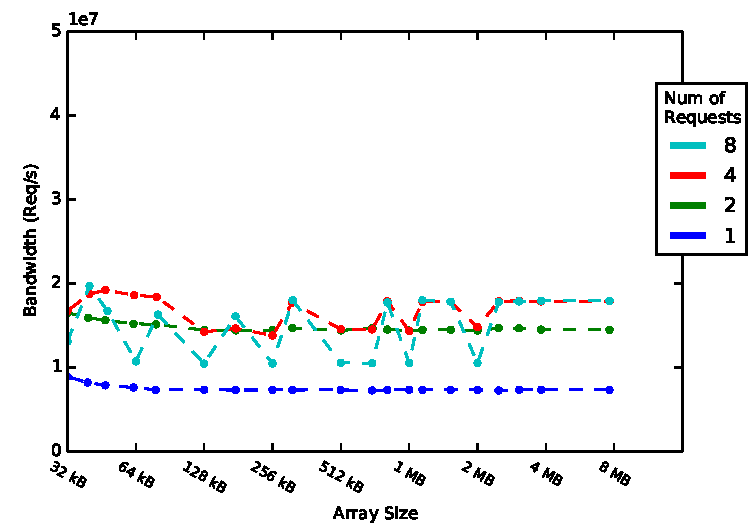
\includegraphics[width=\textwidth]{figures/ccbench_bw2.pdf}
% 	\caption{DRAM Bandwidth = 2}
% \end{subfigure}
% \begin{subfigure}[t]{0.33\textwidth}
% 	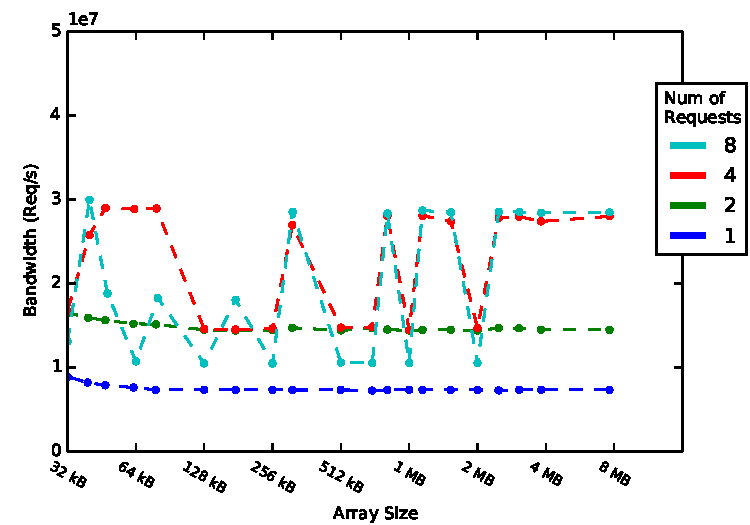
\includegraphics[width=\textwidth]{figures/ccbench_bw4.pdf}
% 	\caption{DRAM Bandwidth = 4}
% \end{subfigure}
% \begin{subfigure}[t]{0.33\textwidth}
% 	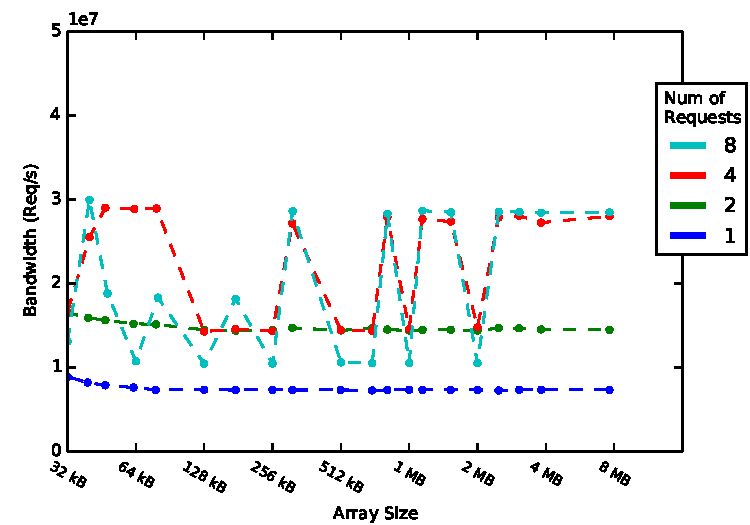
\includegraphics[width=\textwidth]{figures/ccbench_bw8.pdf}
% 	\caption{DRAM Bandwidth = 8}
% \end{subfigure}
% \caption{Bandwidth Validation}
% \label{fig:lat_val}
% \end{figure*}

\begin{figure}[t]
	\centering
	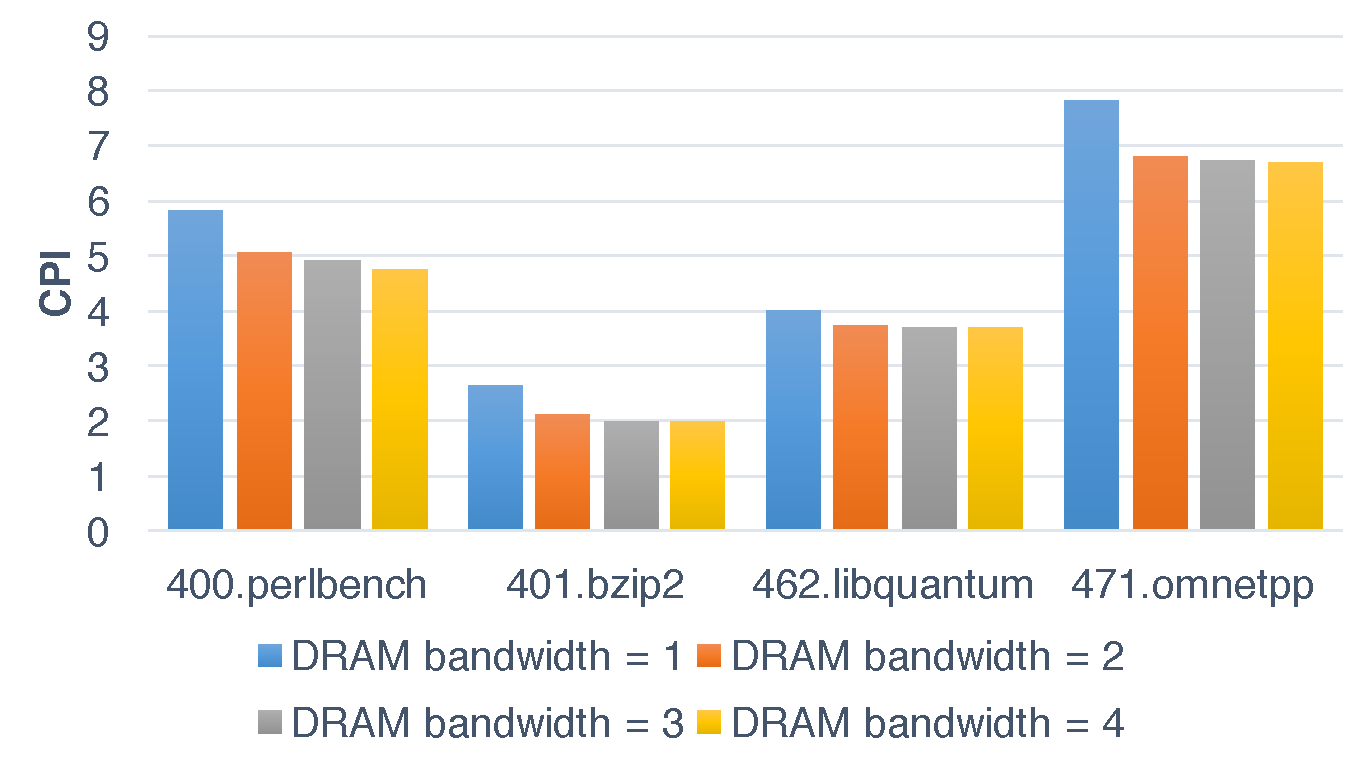
\includegraphics[width=0.8\columnwidth]{figures/boom-bw.pdf}
	\caption{CPIs for BOOM-2w with various bandwidths}
	\label{fig:bandwidths}
\end{figure}

Our next experiment highlights how various memory bandwidths affect the performance of
a superscalar out-of-order processor, assuming the DRAM latency is 100 cycles.
Figure~\ref{fig:bandwidths} shows CPIs for BOOM-2w with various bandwidth 
running \textit{401.bzip2}, \textit{462.libquantum}, and \textit{471.omnetpp}
with the test inputs.
We expect BOOM-2w to be able to issue more memory requests in flight than Rocket,
and thus, we believe memory bandwidth is an important parameter for this case study.
As seen in Figure~\ref{fig:bandwidths}, there is a significant performance
advantage when we increase the memory bandwidth from 1 to 2. However,
the performance benefits diminish as we increase the bandwidth further,
due to lack of memory-level parallelism in the benchmarks.

\subsection{Bank Conflict Model}

\begin{figure}[t]
	\centering
	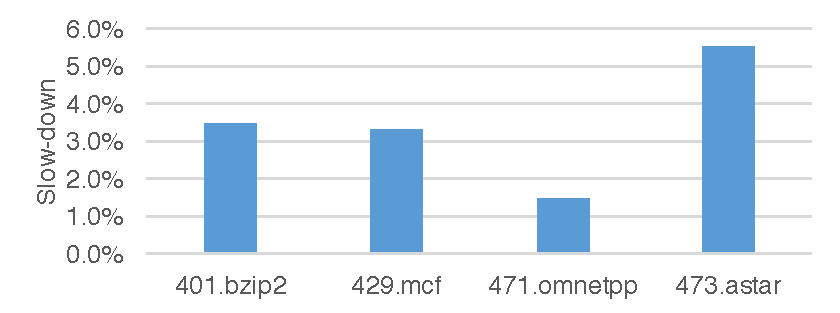
\includegraphics[width=0.8\columnwidth]{figures/boom-bc.pdf}
	\caption{Performance degradation from bank conflicts with 8 banks and a 20-cycle penalty}
	\label{fig:bank_conflict}
\end{figure}

Figure~\ref{fig:bank_conflict} shows how bank conflicts degrade the processor performance.
We run the benchmarks on BOOM-2w with a 8-bank DRAM by varying the bank conflict penalty 
from 1 cycle to 20 cycles. We can see the benchmarks suffer from performance degradation
due to bank conflicts as expected.

\subsection{FCFS MAS Model}

\begin{figure}[t]
		\centering
		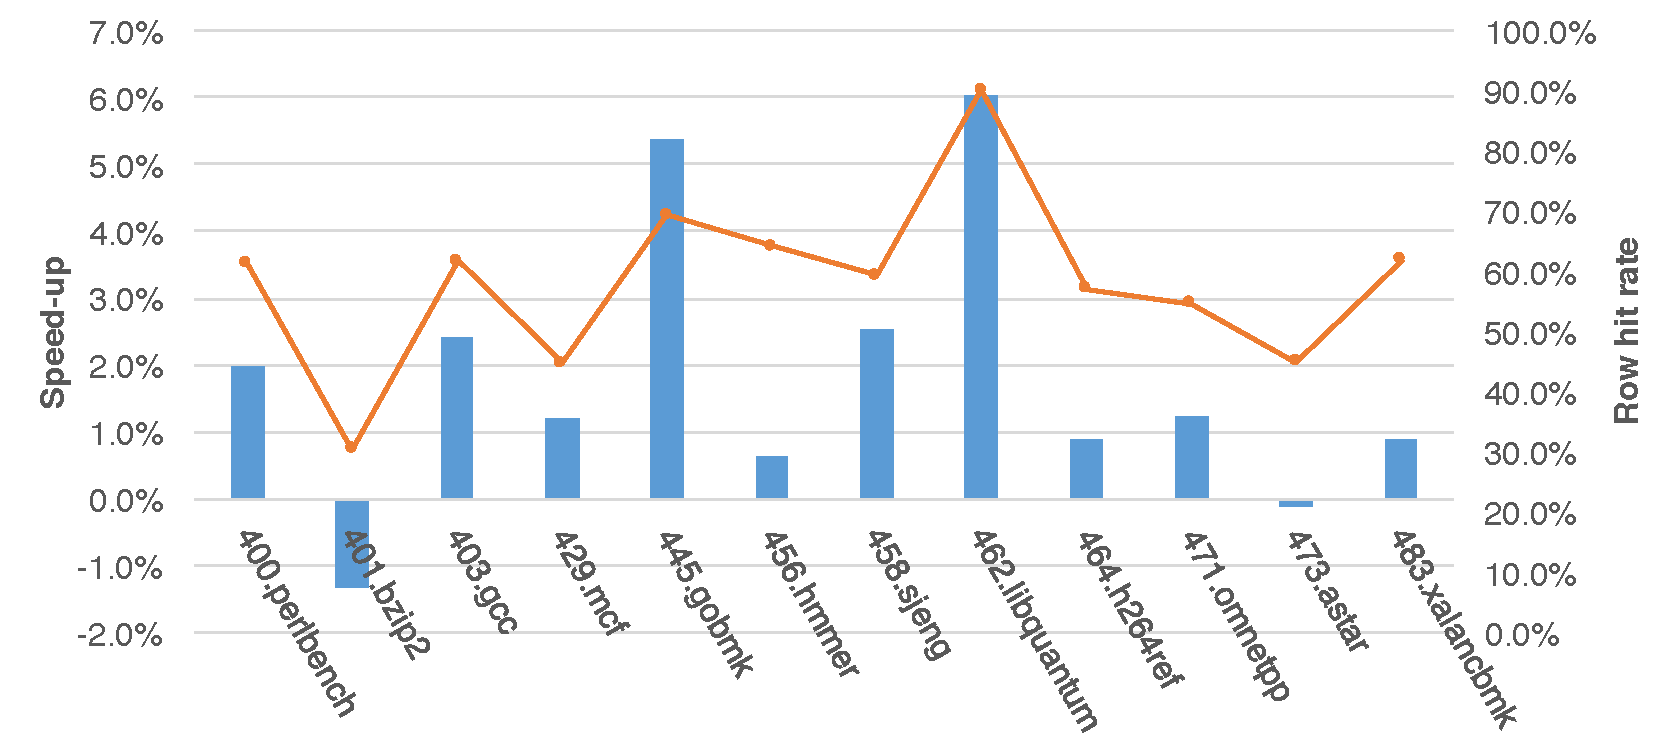
\includegraphics[width=\columnwidth]{figures/rocket-fifomas.pdf}
		\caption{Speedup of the open-page FCFS MAS policy over the close-page policy for Rocket}
		\label{fig:rocket_fifo_mas}
\end{figure}

This section shows the performance impacts of the page policies with the FCFS MAS model
(Section~\ref{sec:timing_model}). This represents a more complex policy, and we contrast variants with open and close row policies.

\begin{table}[t]
\centering
\resizebox{0.7\columnwidth}{!}{%
\begin{tabular}{|c|c c|}
\hline
\textbf{Parameter} & \textbf{Open Policy} & \textbf{Close Policy} \\
\hline
\textit{number of banks} & 8 & 8 \\
\textit{bank address offset} & \textbf{13} & \textbf{6} \\
\textit{row address offsets} & 16 & 16 \\
\textit{bandwidth} & 8 & 8 \\
\textit{tRC} & 7 cycles & 7 cycles \\
\textit{tRCD} & 7 cycles & 7 cycles\\
\textit{tCAS} & 7 cycles & 7 cycles \\
\hline
\end{tabular}}
\caption{FIFO MAS Parameters}
\label{tbl:fifo_mas}
\end{table}

Table~\ref{tbl:fifo_mas} lists the parameter values used in this experiment.
Figure~\ref{fig:rocket_fifo_mas} shows the speedup of the open page policy over the close page
policy for the SPEC benchmarks and the DaCapo benchmarks running on Rocket, along with the row
hit rate for each benchmark. Overall, the open page policy has perfomance benefits for the SPEC
CPU integer benchmarks except for \textit{402.bzip2} and \textit{473.astar}. As indicated in
Figure~\ref{fig:rocket_fifo_mas}, the memory requests of \textit{402.bzip2} and
\textit{473.astar} lack locality (resulting in low row hit rates), which explains these results.


\chapter{Java Case Study}

\begin{figure*}
	\centering
	\begin{subfigure}[t]{0.32\textwidth}
		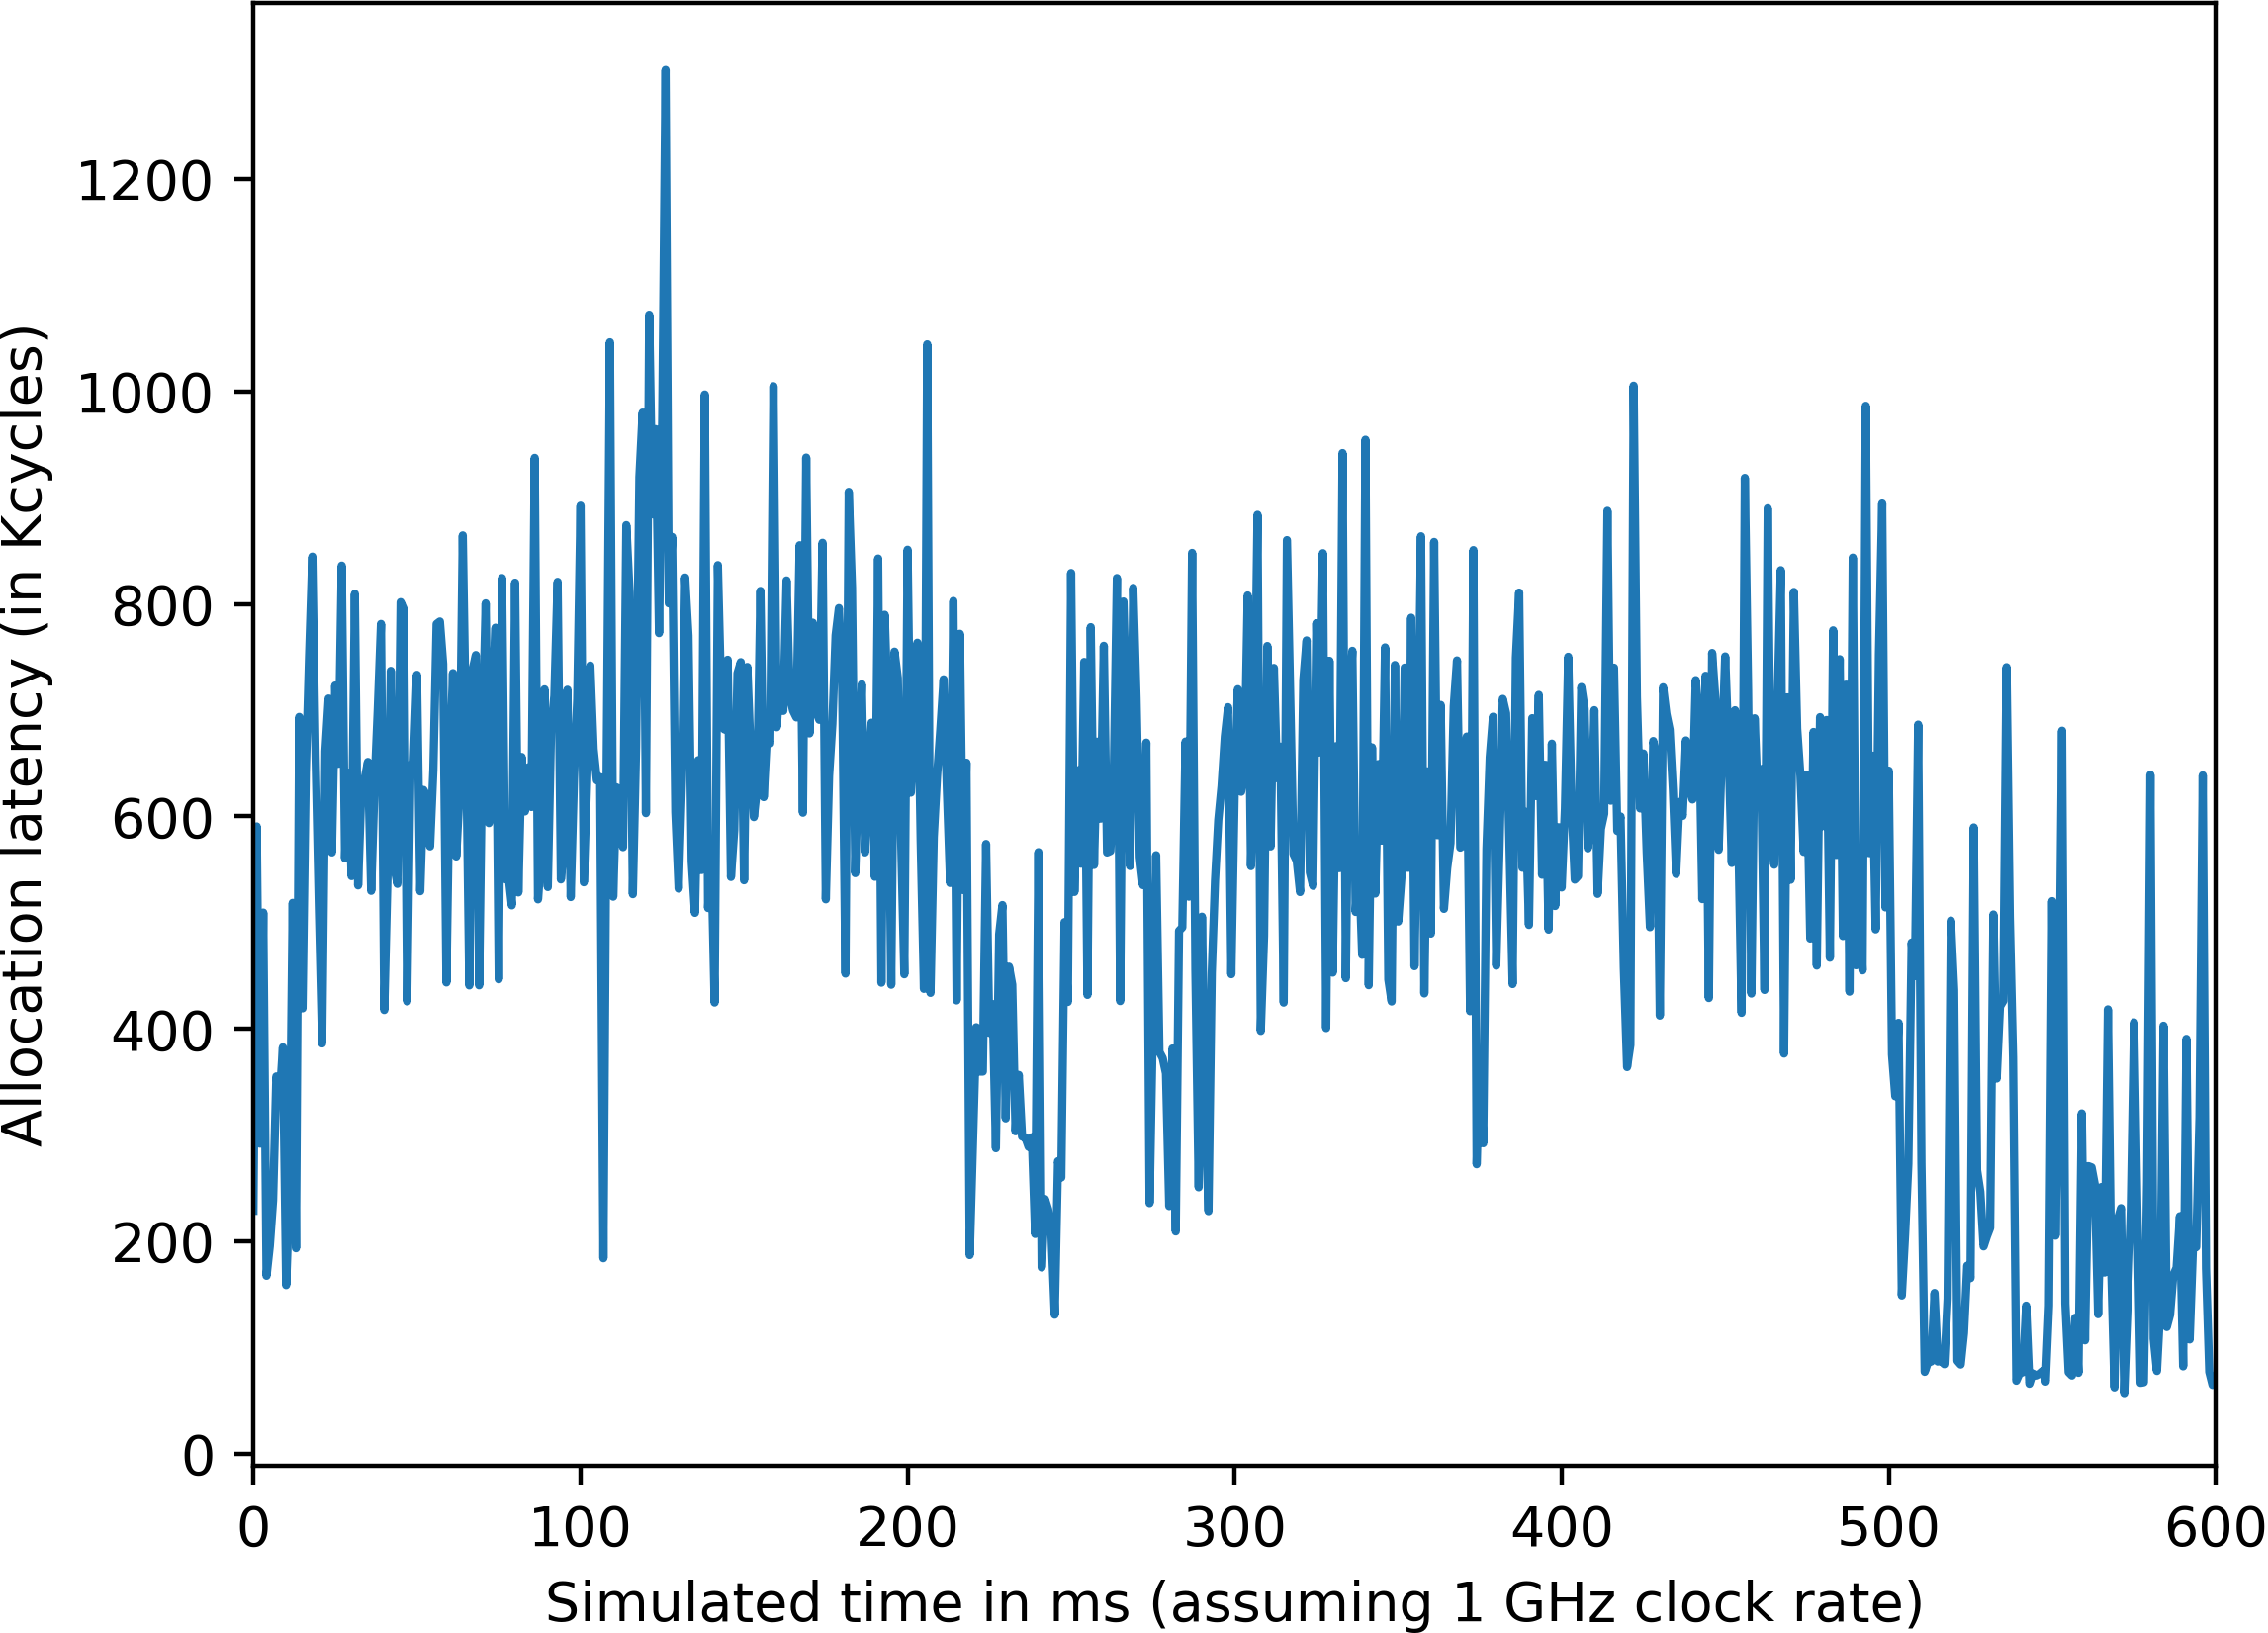
\includegraphics[width=\textwidth]{results/java-alloc-macro.png}
		\caption{The first 600ms of execution sampled at 1 KHz}
	\end{subfigure}
	\begin{subfigure}[t]{0.32\textwidth}
		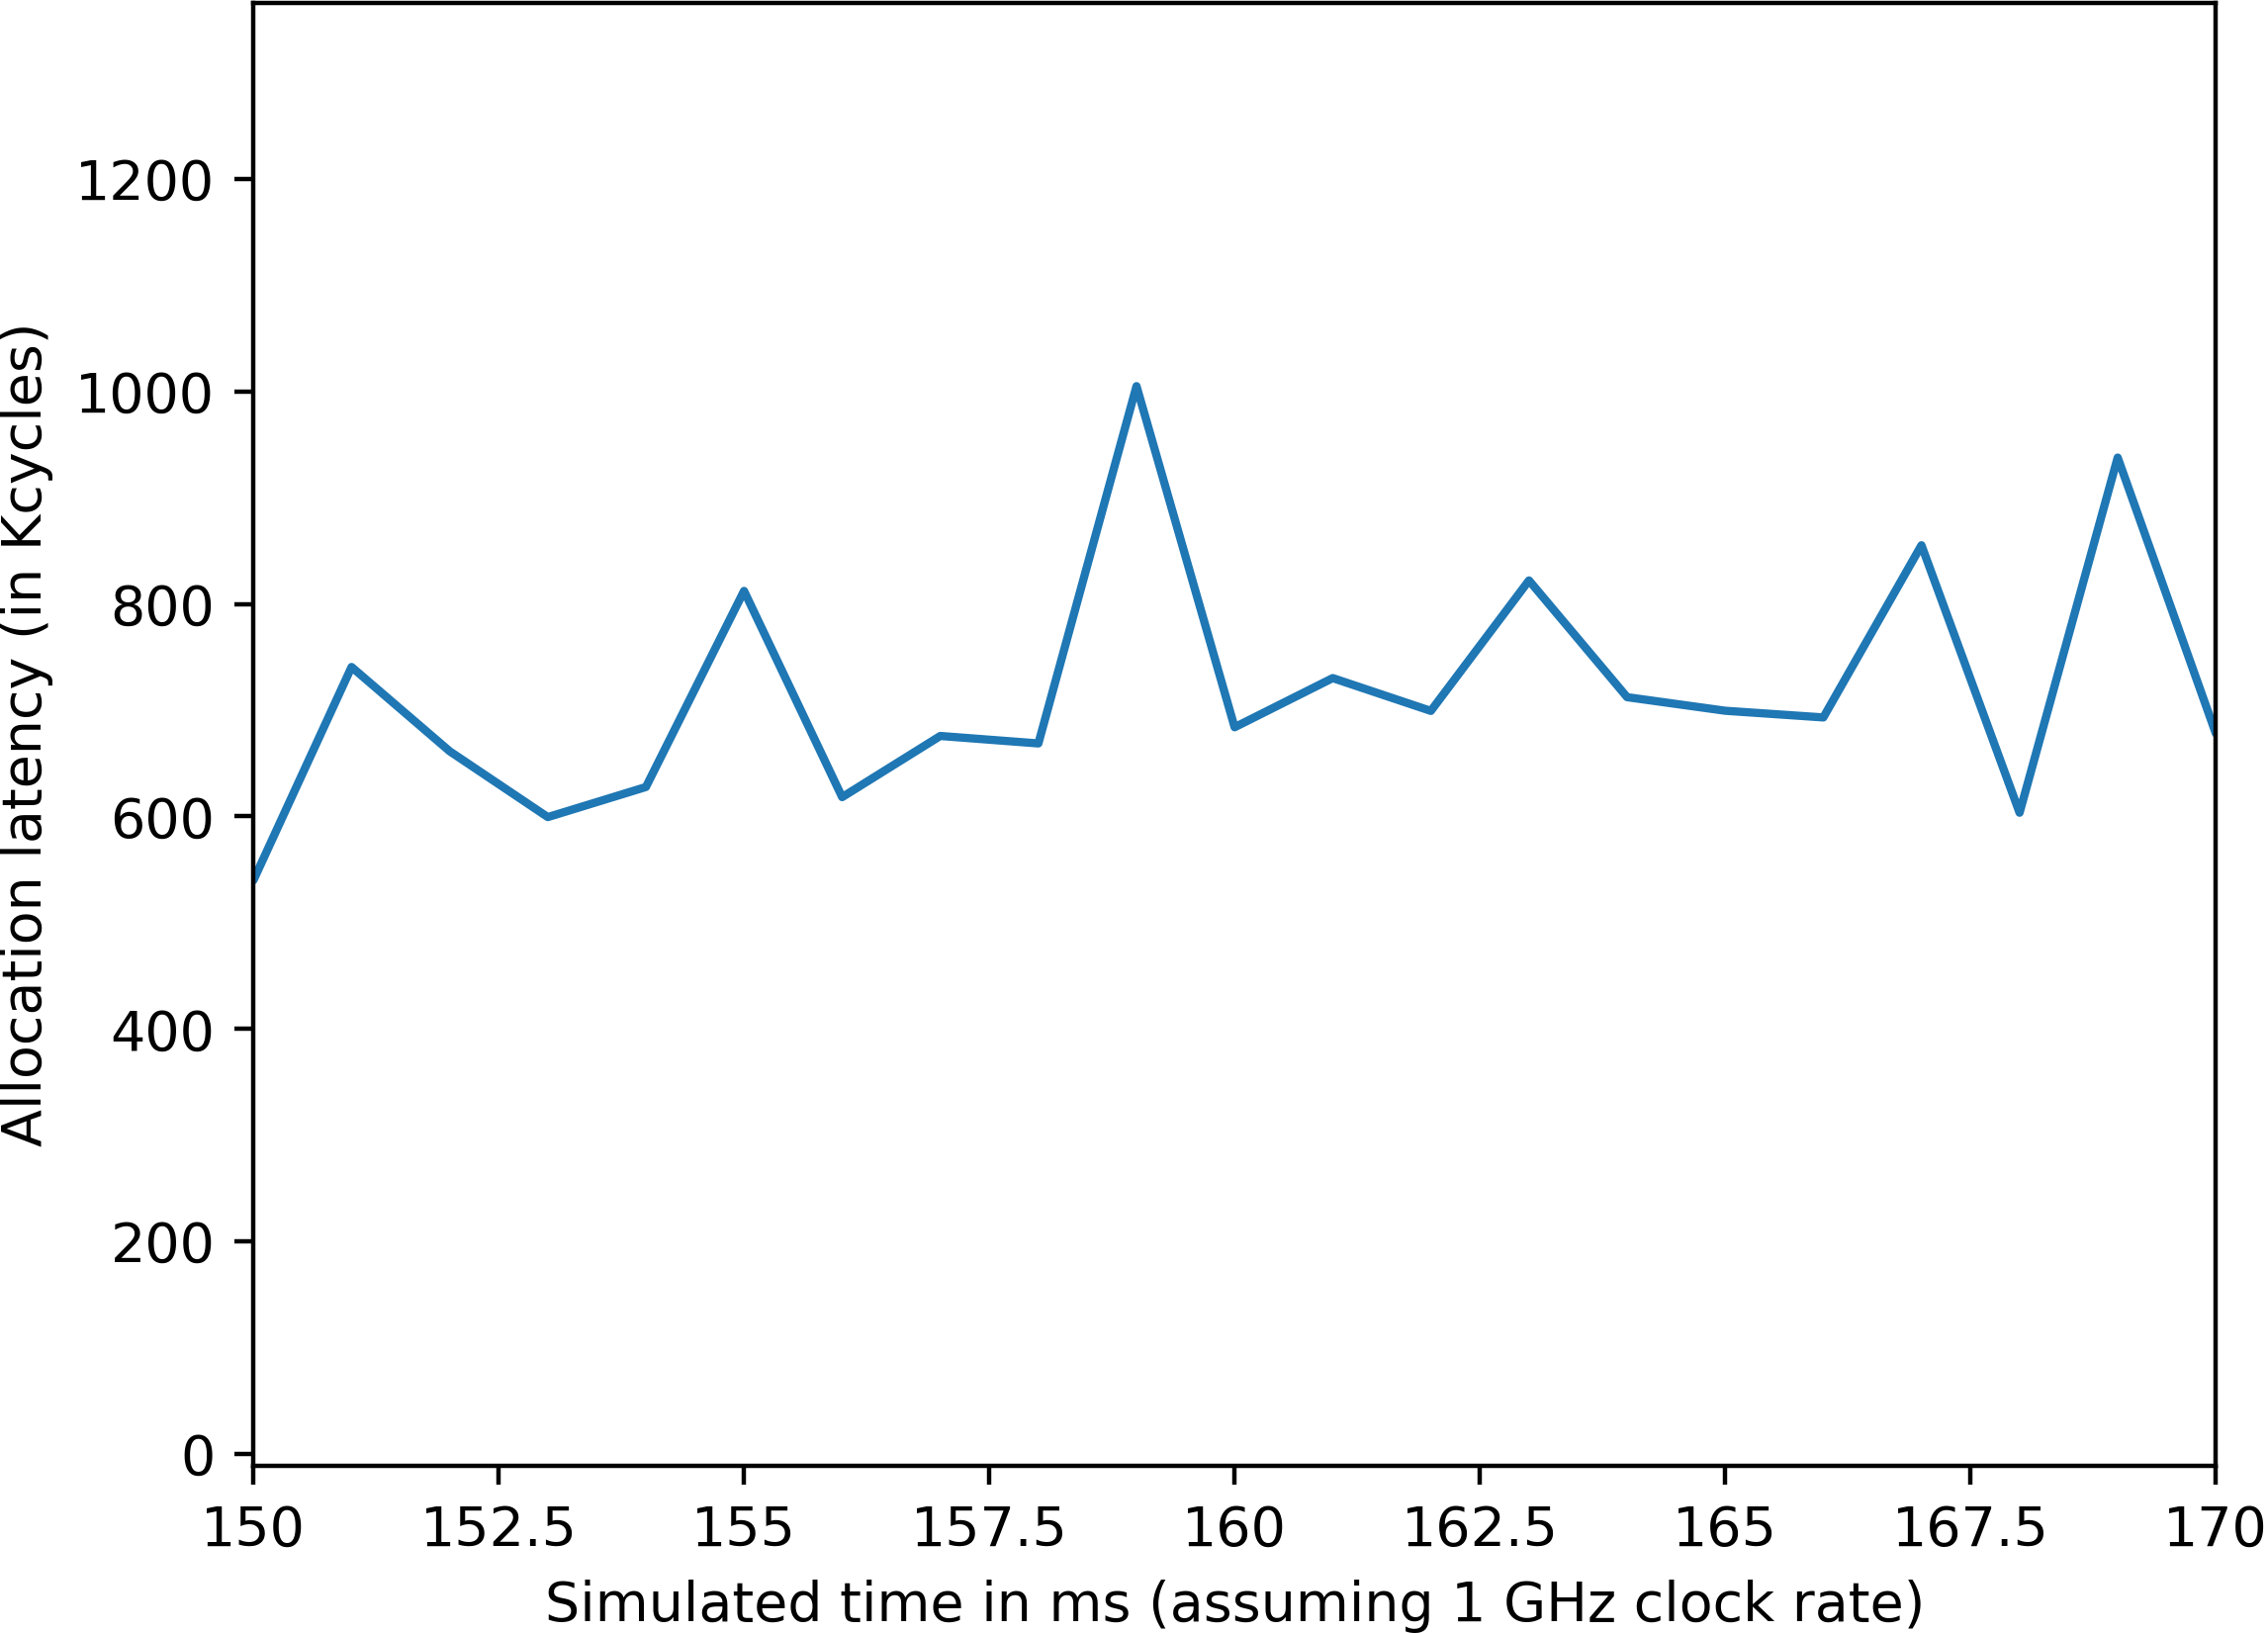
\includegraphics[width=\textwidth]{results/java-alloc-1khz.png}
		\caption{20ms slice sampled at 1 KHz}
	\end{subfigure}
	\begin{subfigure}[t]{0.32\textwidth}
		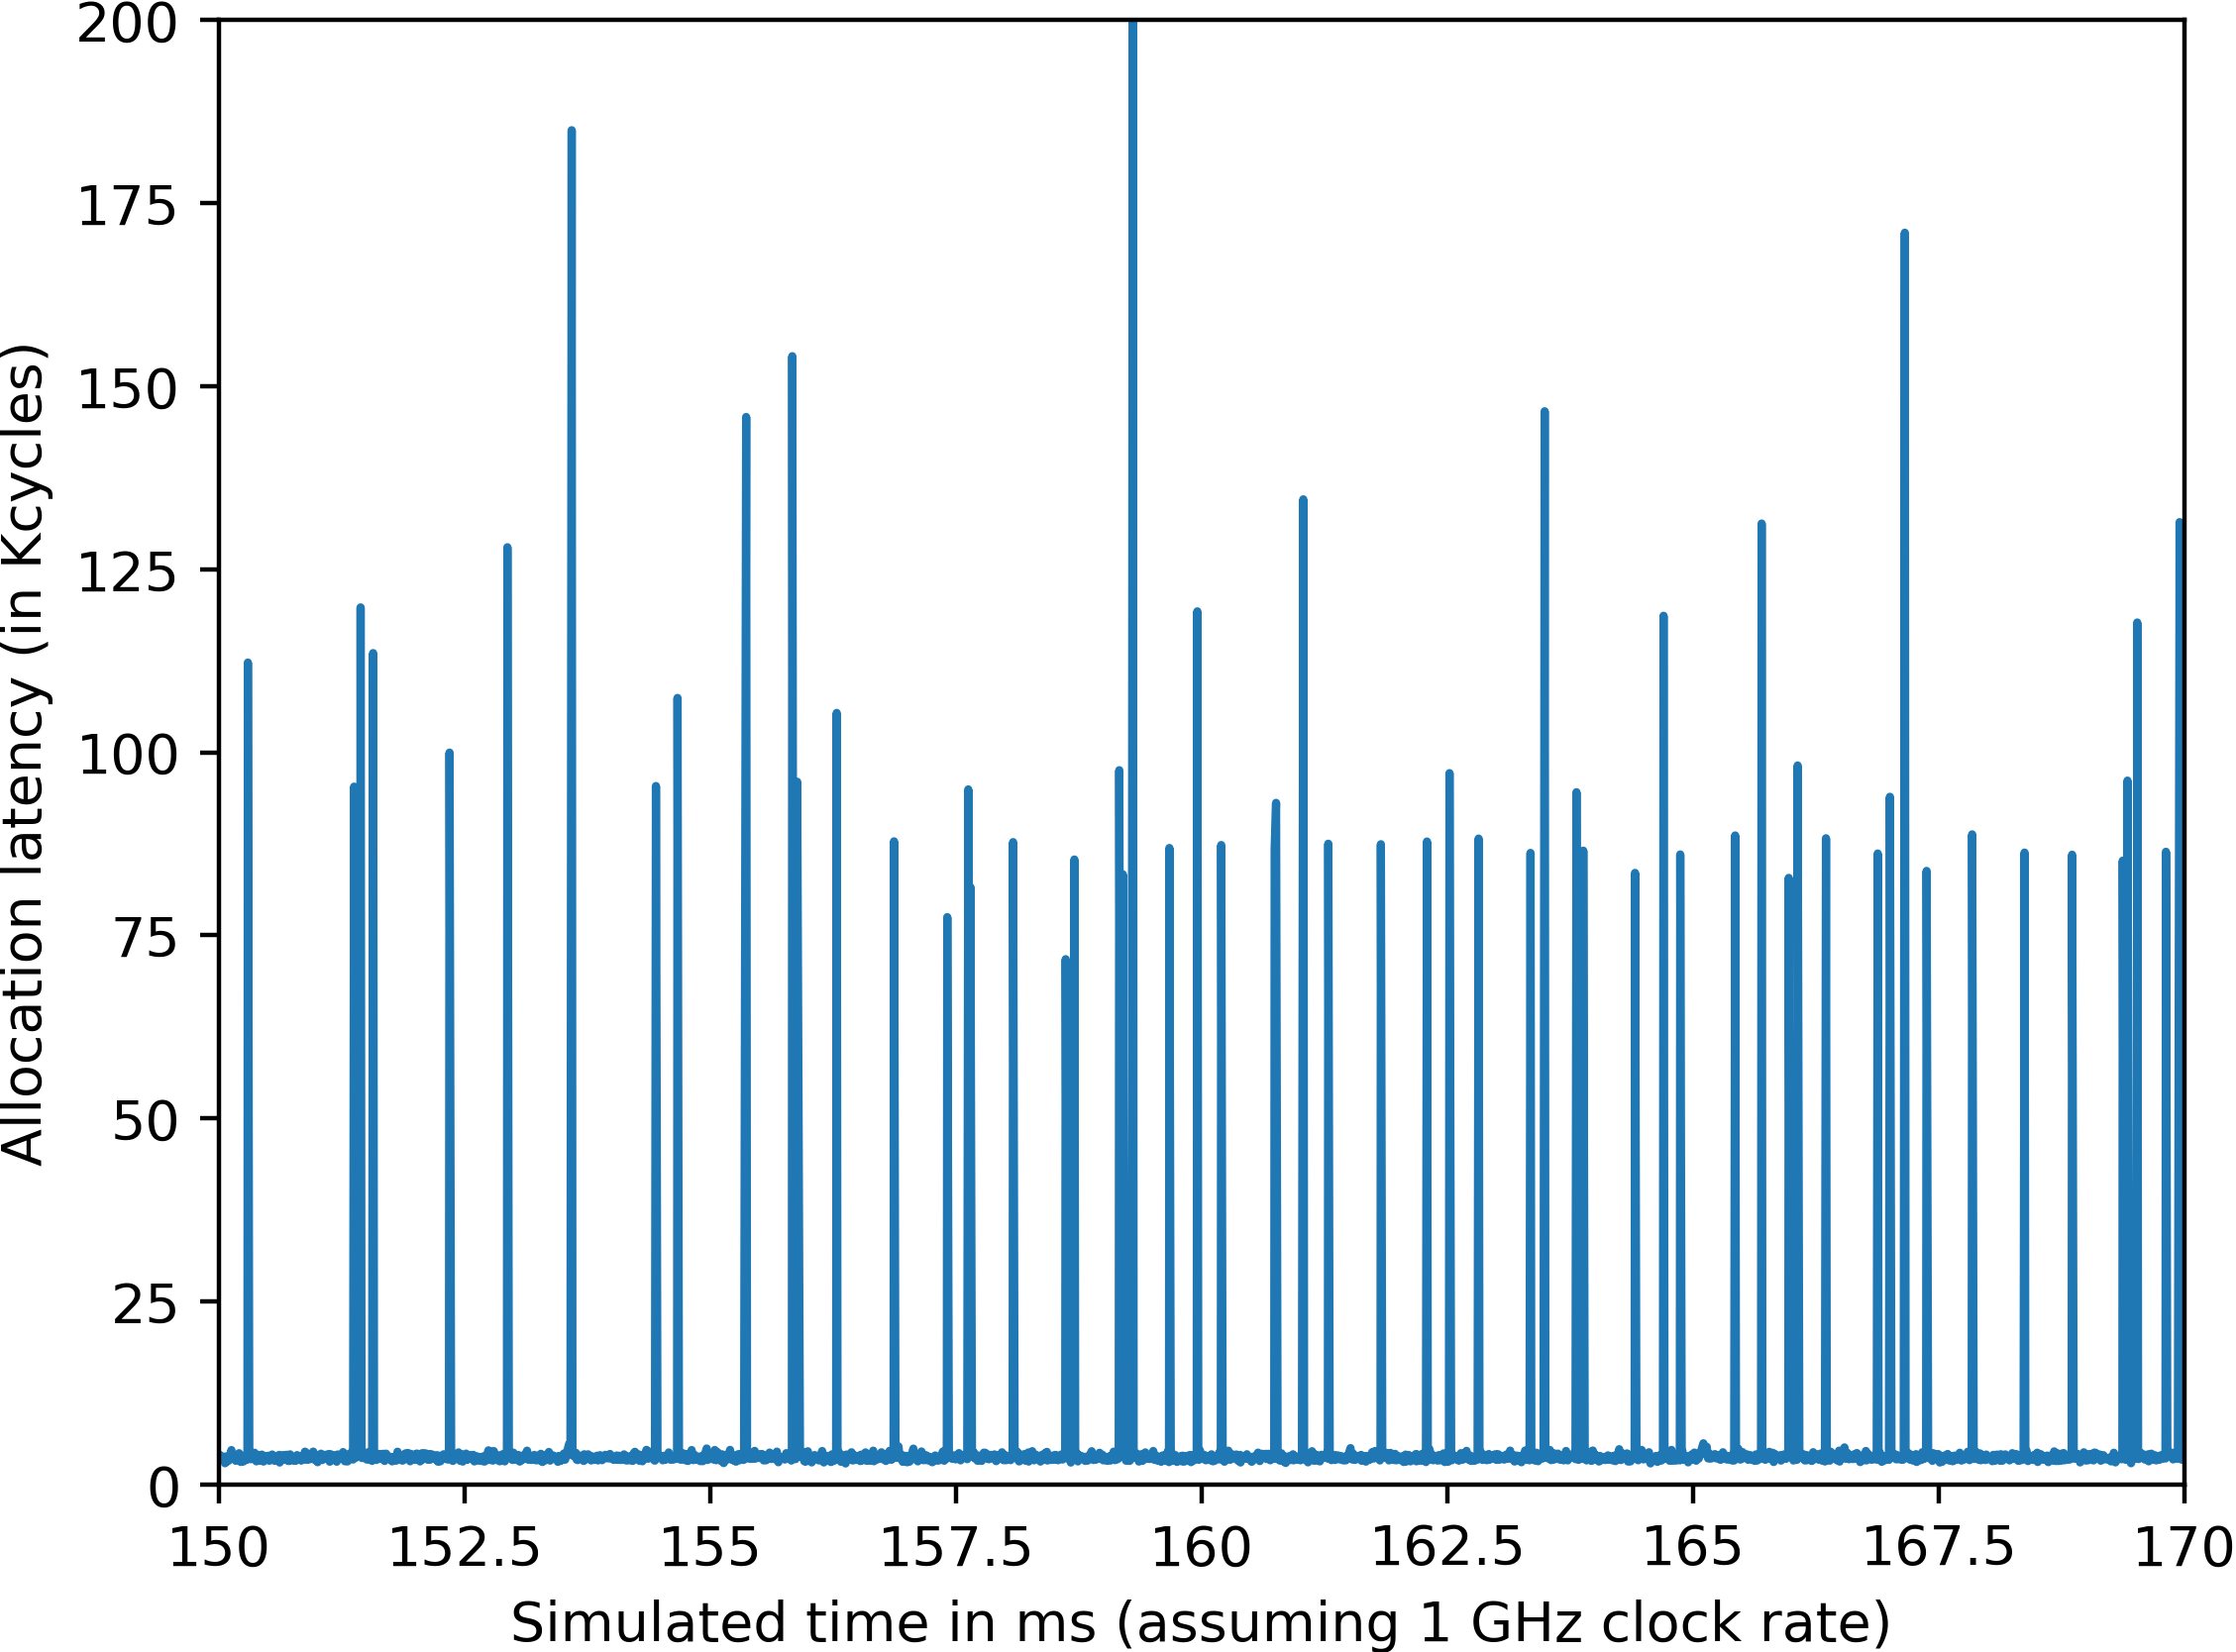
\includegraphics[width=\textwidth]{results/java-alloc-detailed.png}
		\caption{Trace of the same 20ms on our platform}
	\end{subfigure}
	\caption{Contrasting an approach that aggregates time spent in allocation at a 1 KHz-granularity with recording every allocation in hardware without introducing observer effects to the application (numbers are from the \texttt{pmd} Dacapo benchmark).}
	\label{fig:java_alloc}
\end{figure*}

Managed languages such as Java, C\# or Python are widely used and a large
amount of research focuses on improving the language runtime systems that
underpin these languages. Previous work suggests that managed-language runtimes
can substantially benefit from hardware support and hardware-software co-design
\cite{Click:2005:PGA:1064979.1064988,Wright:2005:OMA:1698178,Ungar:1984:ASS:800015.808182,Joao:2009:FRH:1555754.1555806}.


\begin{figure}[t]
		\centering
		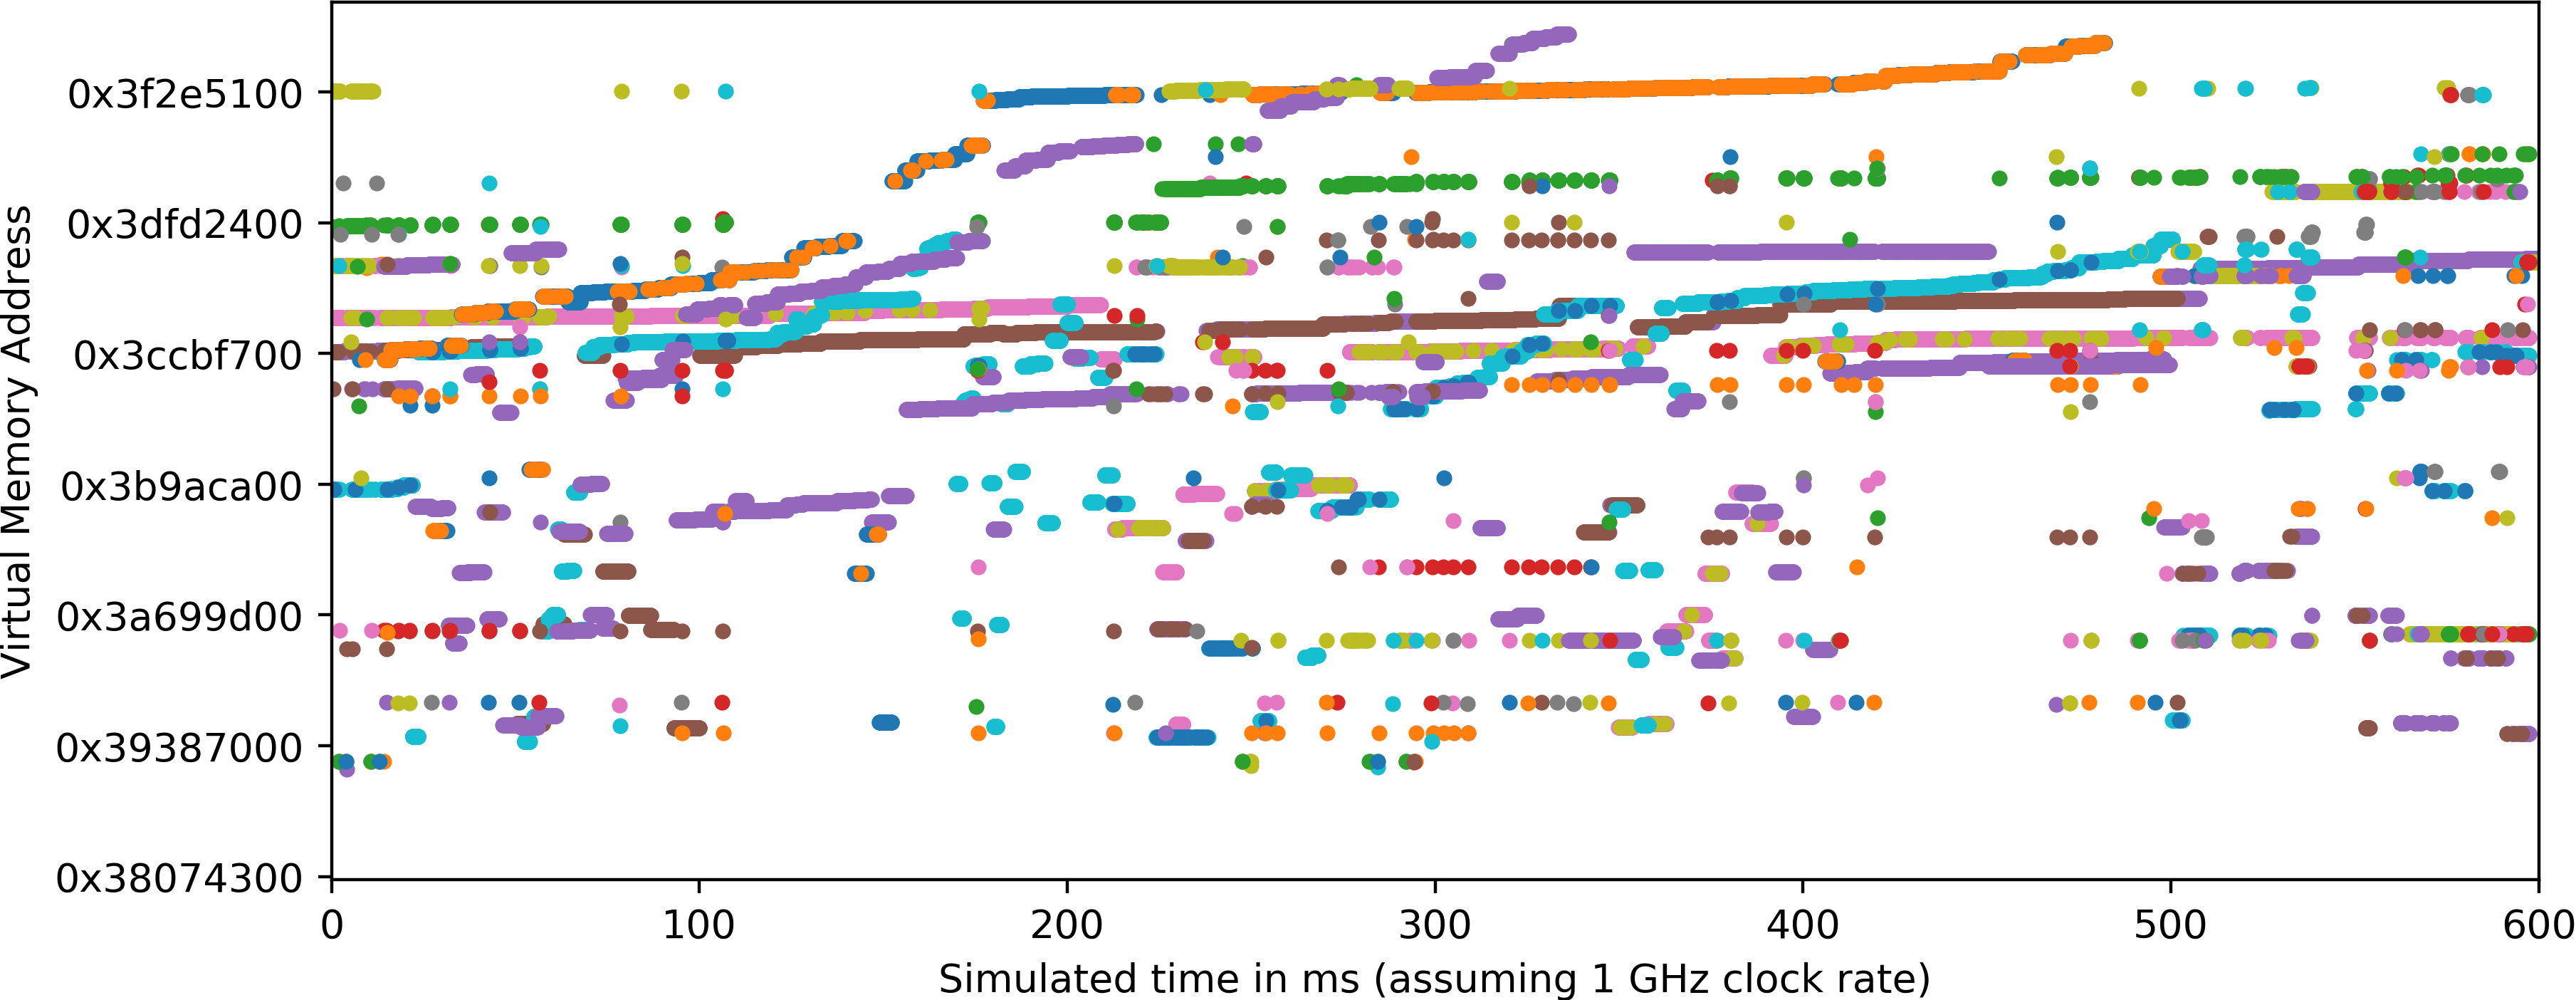
\includegraphics[width=\columnwidth]{results/heatmap.png}
		\caption{Addresses returned by the JikesRVM free-list allocator. Colors indicate the allocation size class.}
		\label{fig:java_alloc_heatmap}
\end{figure}

However, evaluating this work without building out the full system is
challenging, as the interactions between hardware and software are often very
fine-grained and can therefore only be captured in high-fidelity simulation.
For example, concurrent garbage collectors incur most of their overheads from
code sequences that individually only account for 10 or less cycles, but occur
on every reference access \cite{Click:2005:PGA:1064979.1064988}. In a different
line of work, Yang et al. demonstrated that sampling Java applications at 100
KHz or less misses many important performance characteristics
\cite{Yang:2015:CPM:2749469.2750401}.


\begin{figure}[t]
		\centering
		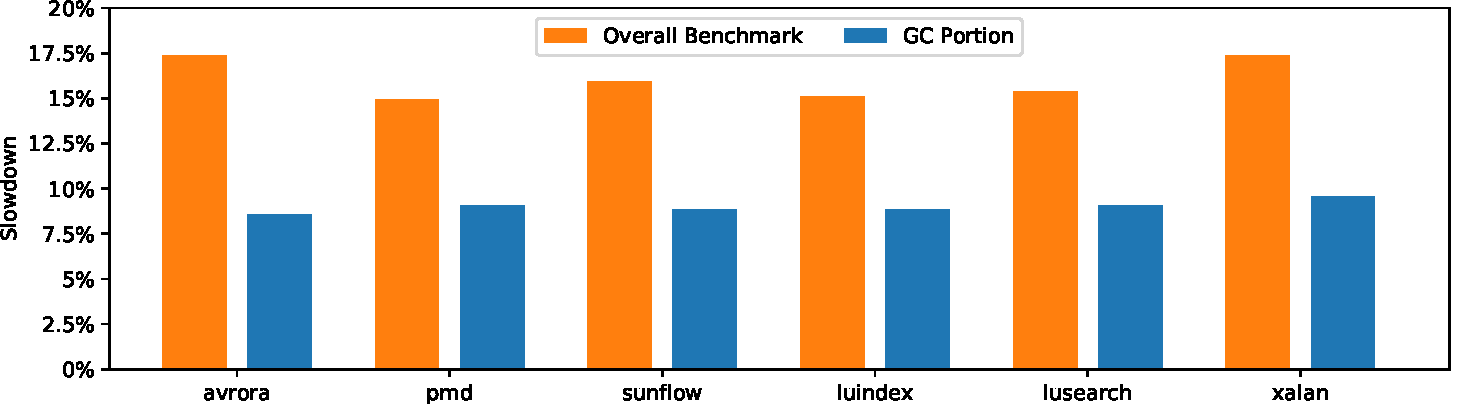
\includegraphics[width=\columnwidth]{results/dacapo-varymodel.pdf}
		\caption{Slowdown of increasing DRAM latency by a factor of 2$\times$. Breaking out the data into GC and non-GC portion shows us that the GC is less sensitive to long memory latencies than the rest of the execution.}
		\label{fig:dacapo_latency2x}
\end{figure}

While high-fidelity software simulators would solve these problems, managed
workloads run across a large number of threads and require full-system support,
which makes them unsuitable for existing simulators. Java workloads in
particular also have very large memory footprints. As a result, extensive
design space explorations that involve managed languages are rare, and recent
work has instead focused on better measuring existing hardware
\cite{Cao:2012:YYP:2337159.2337185,Yang:2015:CPM:2749469.2750401}.

One example of these types of challenges are exemplified in a paper by Hertz
and Berger \cite{Hertz:2005:QPG:1094811.1094836}. In order to investigate
trade-offs between manual and automatic memory management, the authors had to
instrument an existing system to extract allocated memory addresses, and -- in
a second pass -- inject addresses produced by an oracle. The authors found that
this was difficult to achieve in software, as the software instrumentation led
to a 2-33\% perturbation in execution time, which was larger than the effect
they were trying to measure. They therefore decided to use a software simulator
(Dynamic SimpleScalar) for these experiments. While appropriate in this
setting, the shortcoming of this approach is simulation speed and the
reliability of the resulting numbers.

FPGA simulations, automatically generated from the RTL designs~\cite{strober},
in conjunction with the realistic memory models introduced in this paper,
provide an opportunity to fundamentally address this problem by running on real
hardware that can be modified and enables design space exploration of the
memory and I/O system. The memory system is particularly important, as many
managed-runtime problems are closely interlinked with it (e.g., memory
allocation or GC).

To enable this kind of research, we brought up a full Java Virtual Machine
(JVM) on our platform. We picked the Jikes Research VM
\cite{alpern_jikes_2005}, which is the defacto standard in managed-language
research. We ported JikesRVM and its non-optimizing \emph{Baseline} JIT
compiler to RISC-V. To our knowledge, this is the first full-system platform
for hardware-software research on Java applications, allowing modification of
the software stack, the hardware and the memory system model. Larger FPGAs with
several GBs of DRAM (which only became available recently) were essential in
enabling this. In the following sections, we will describe the types of
experiments that become possible with our platform.


\begin{figure*}
	\centering
	\begin{subfigure}[t]{0.23\textwidth}
		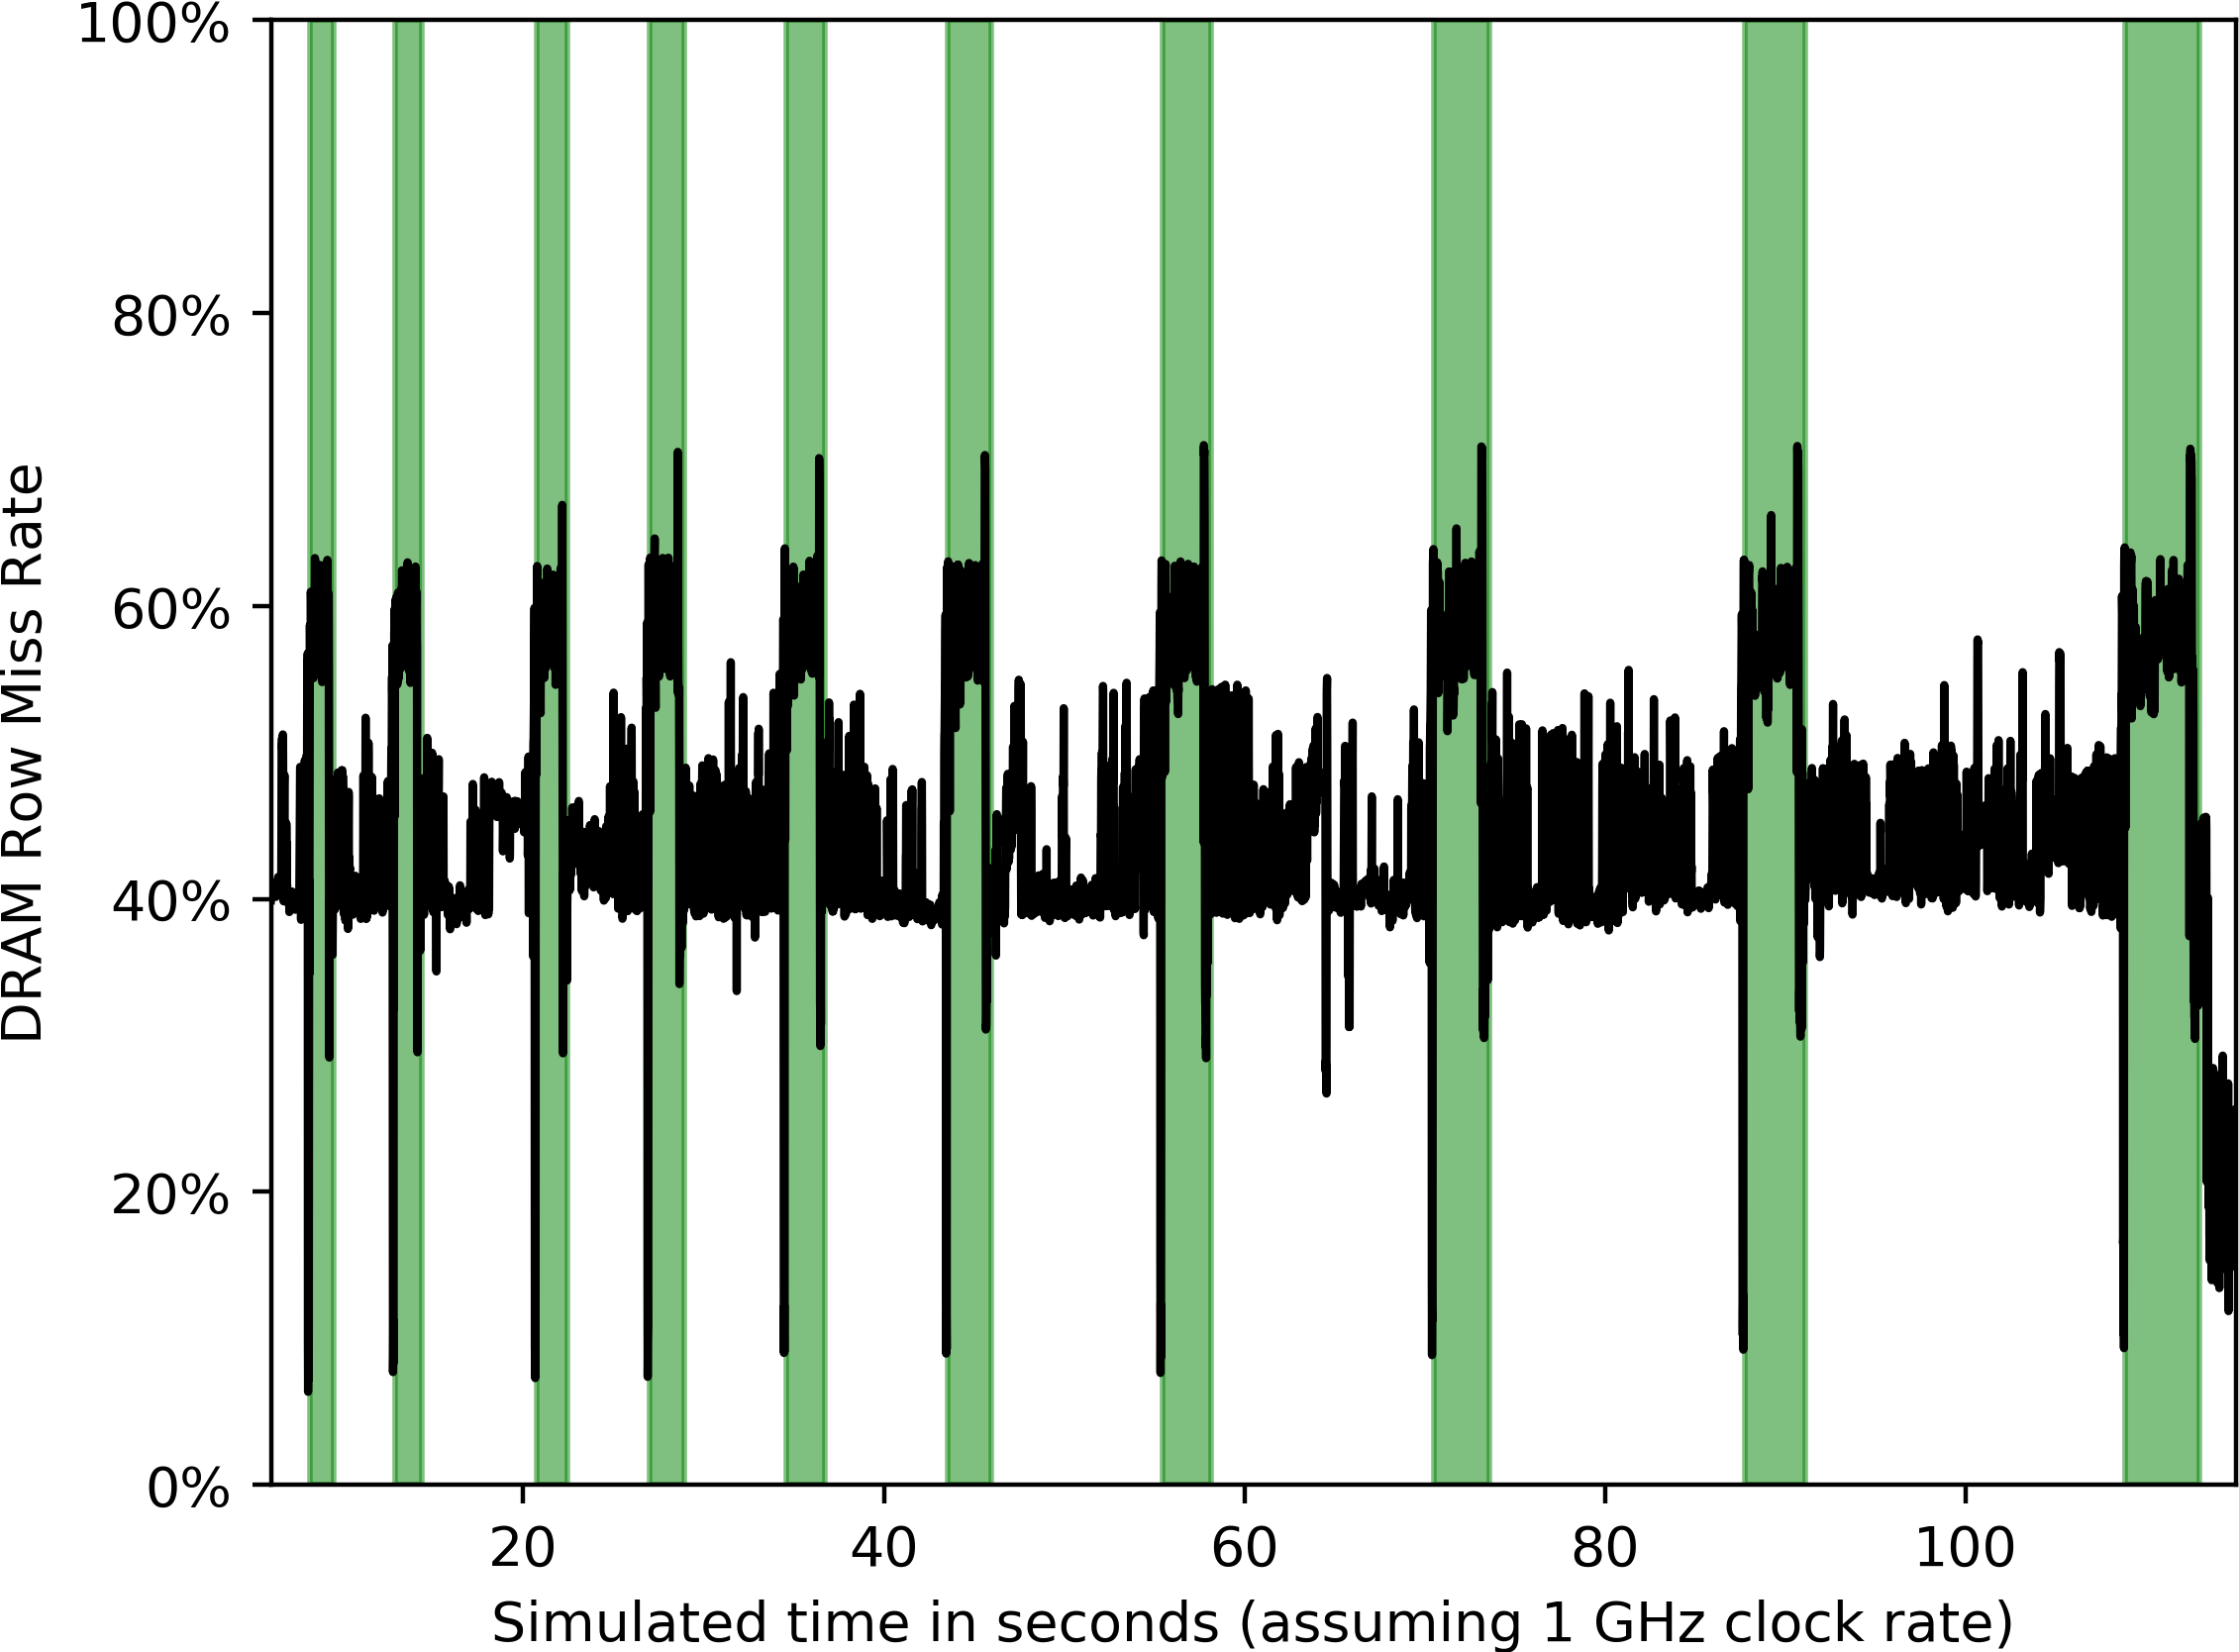
\includegraphics[width=\textwidth]{results/rowmisses_pmd.png}
		\caption{pmd}
	\end{subfigure}
	\begin{subfigure}[t]{0.23\textwidth}
		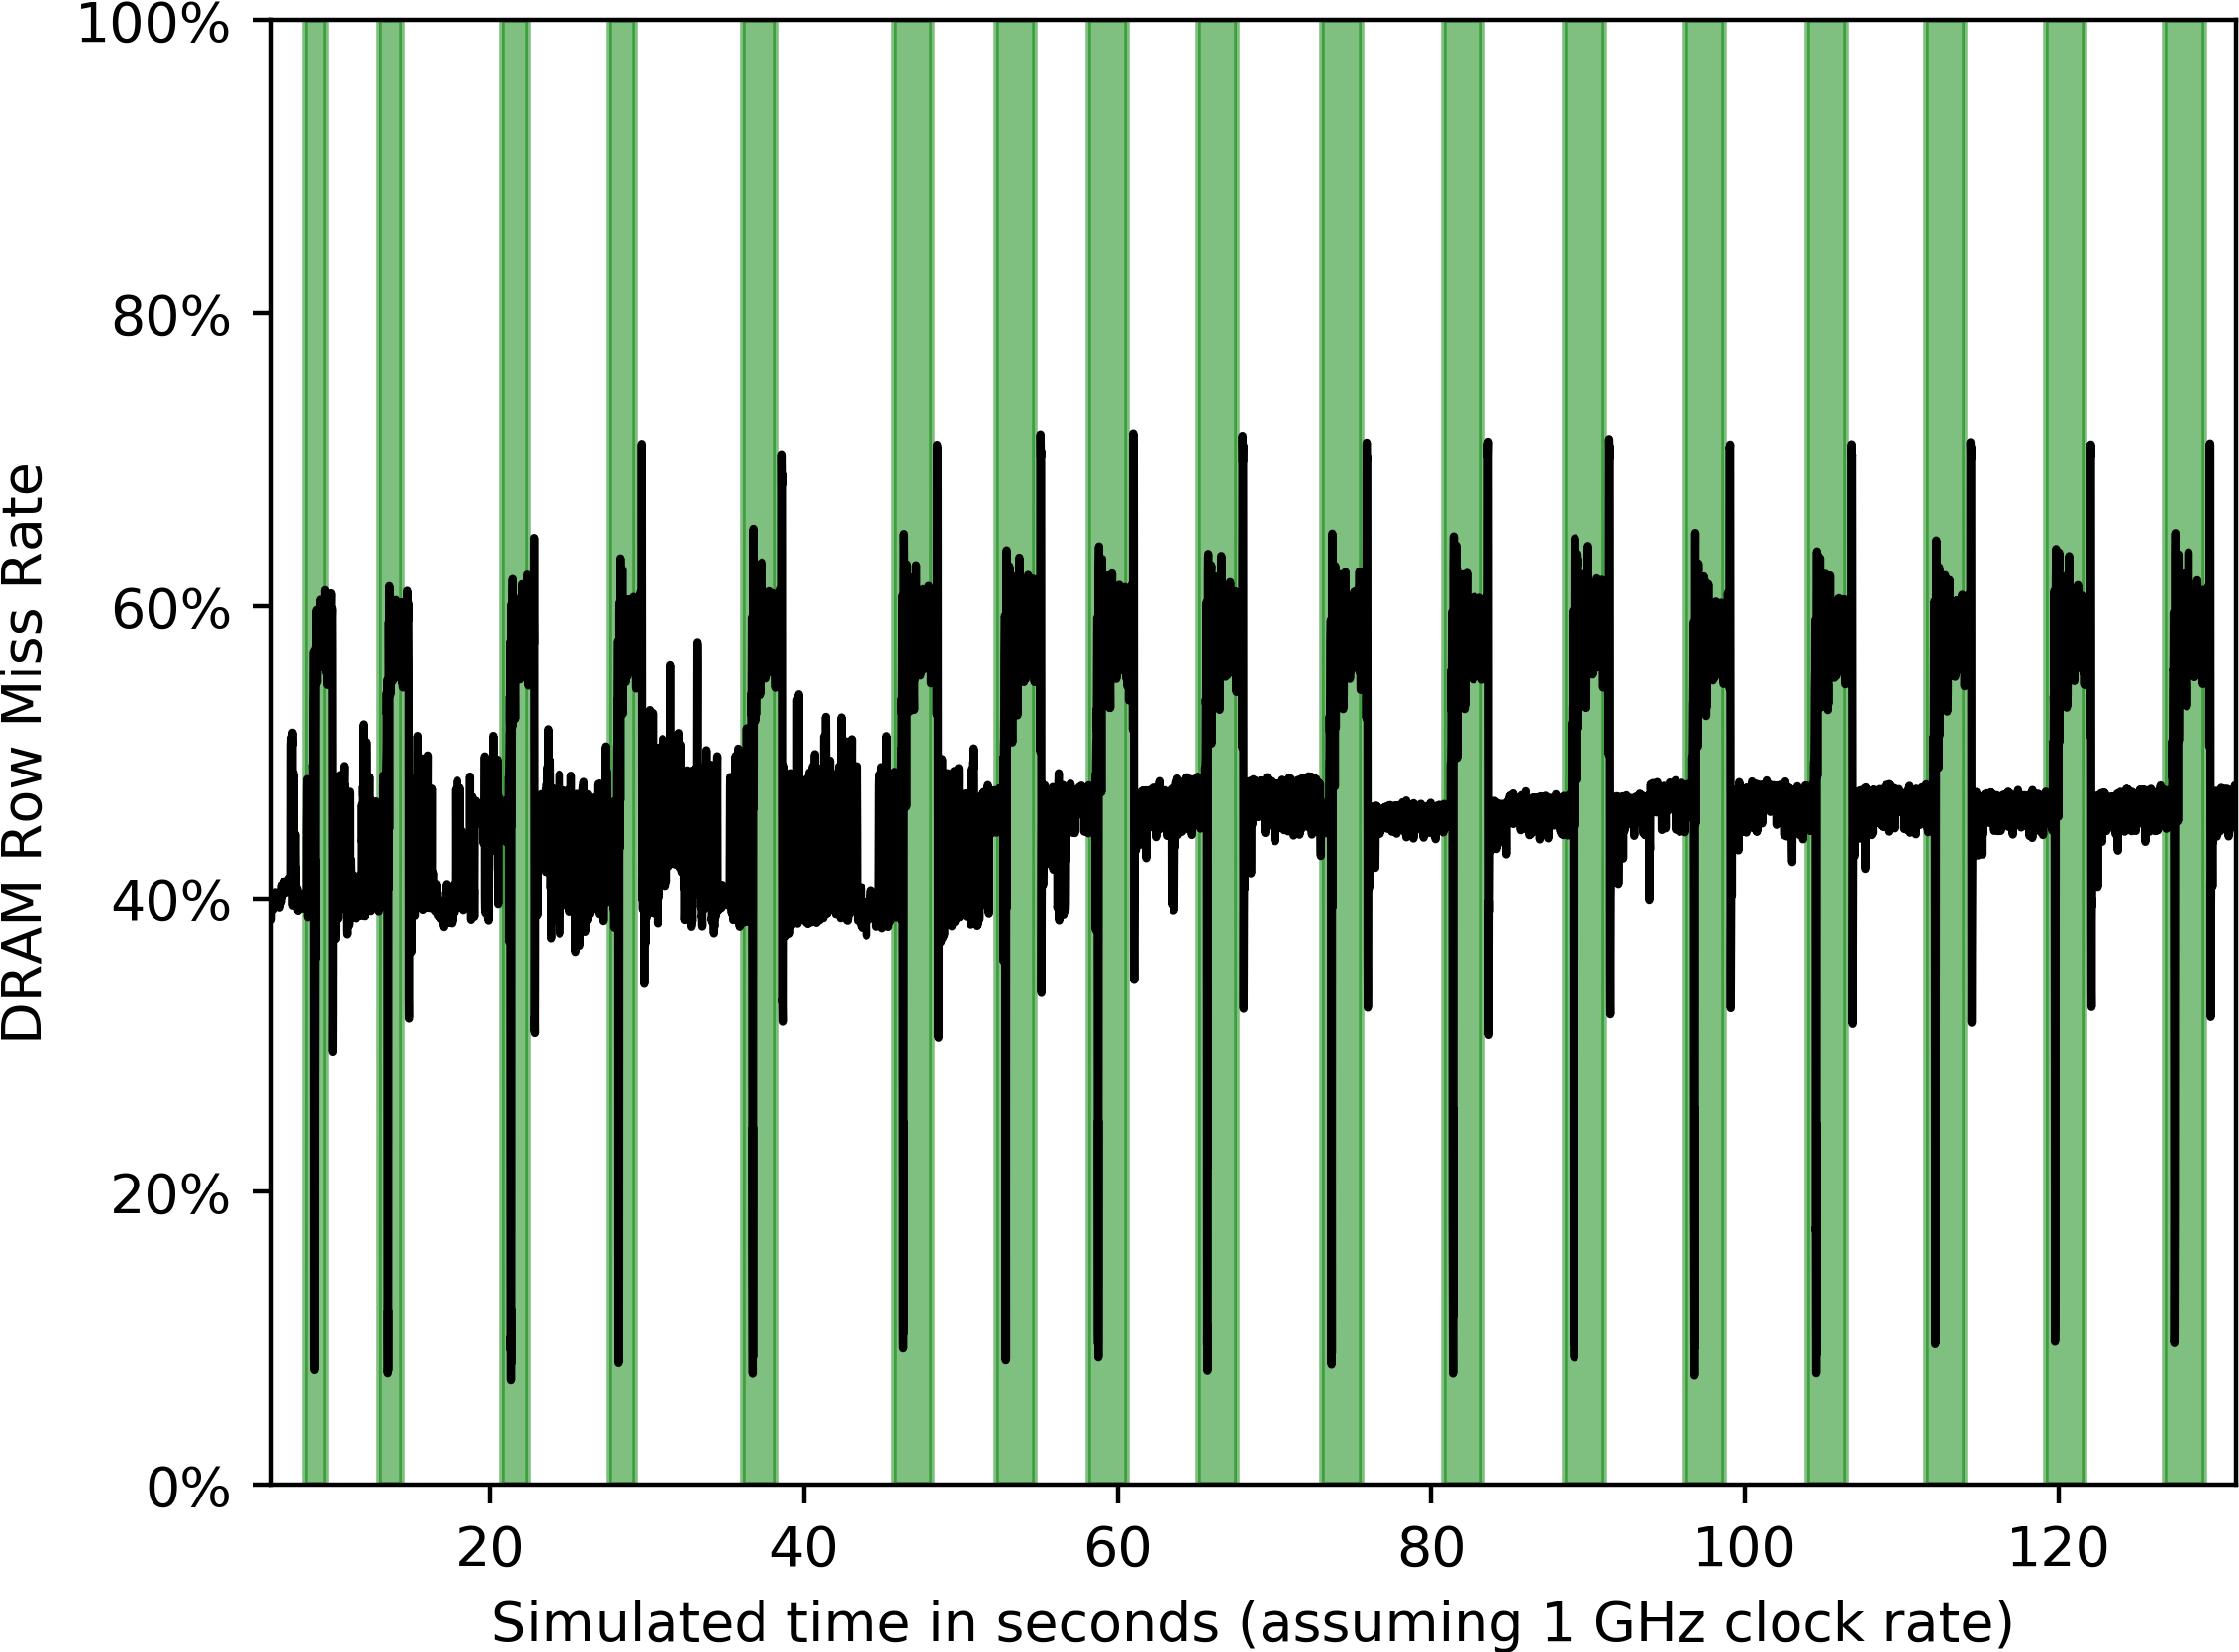
\includegraphics[width=\textwidth]{results/rowmisses_lusearch.png}
		\caption{lusearch}
	\end{subfigure}
	\begin{subfigure}[t]{0.23\textwidth}
		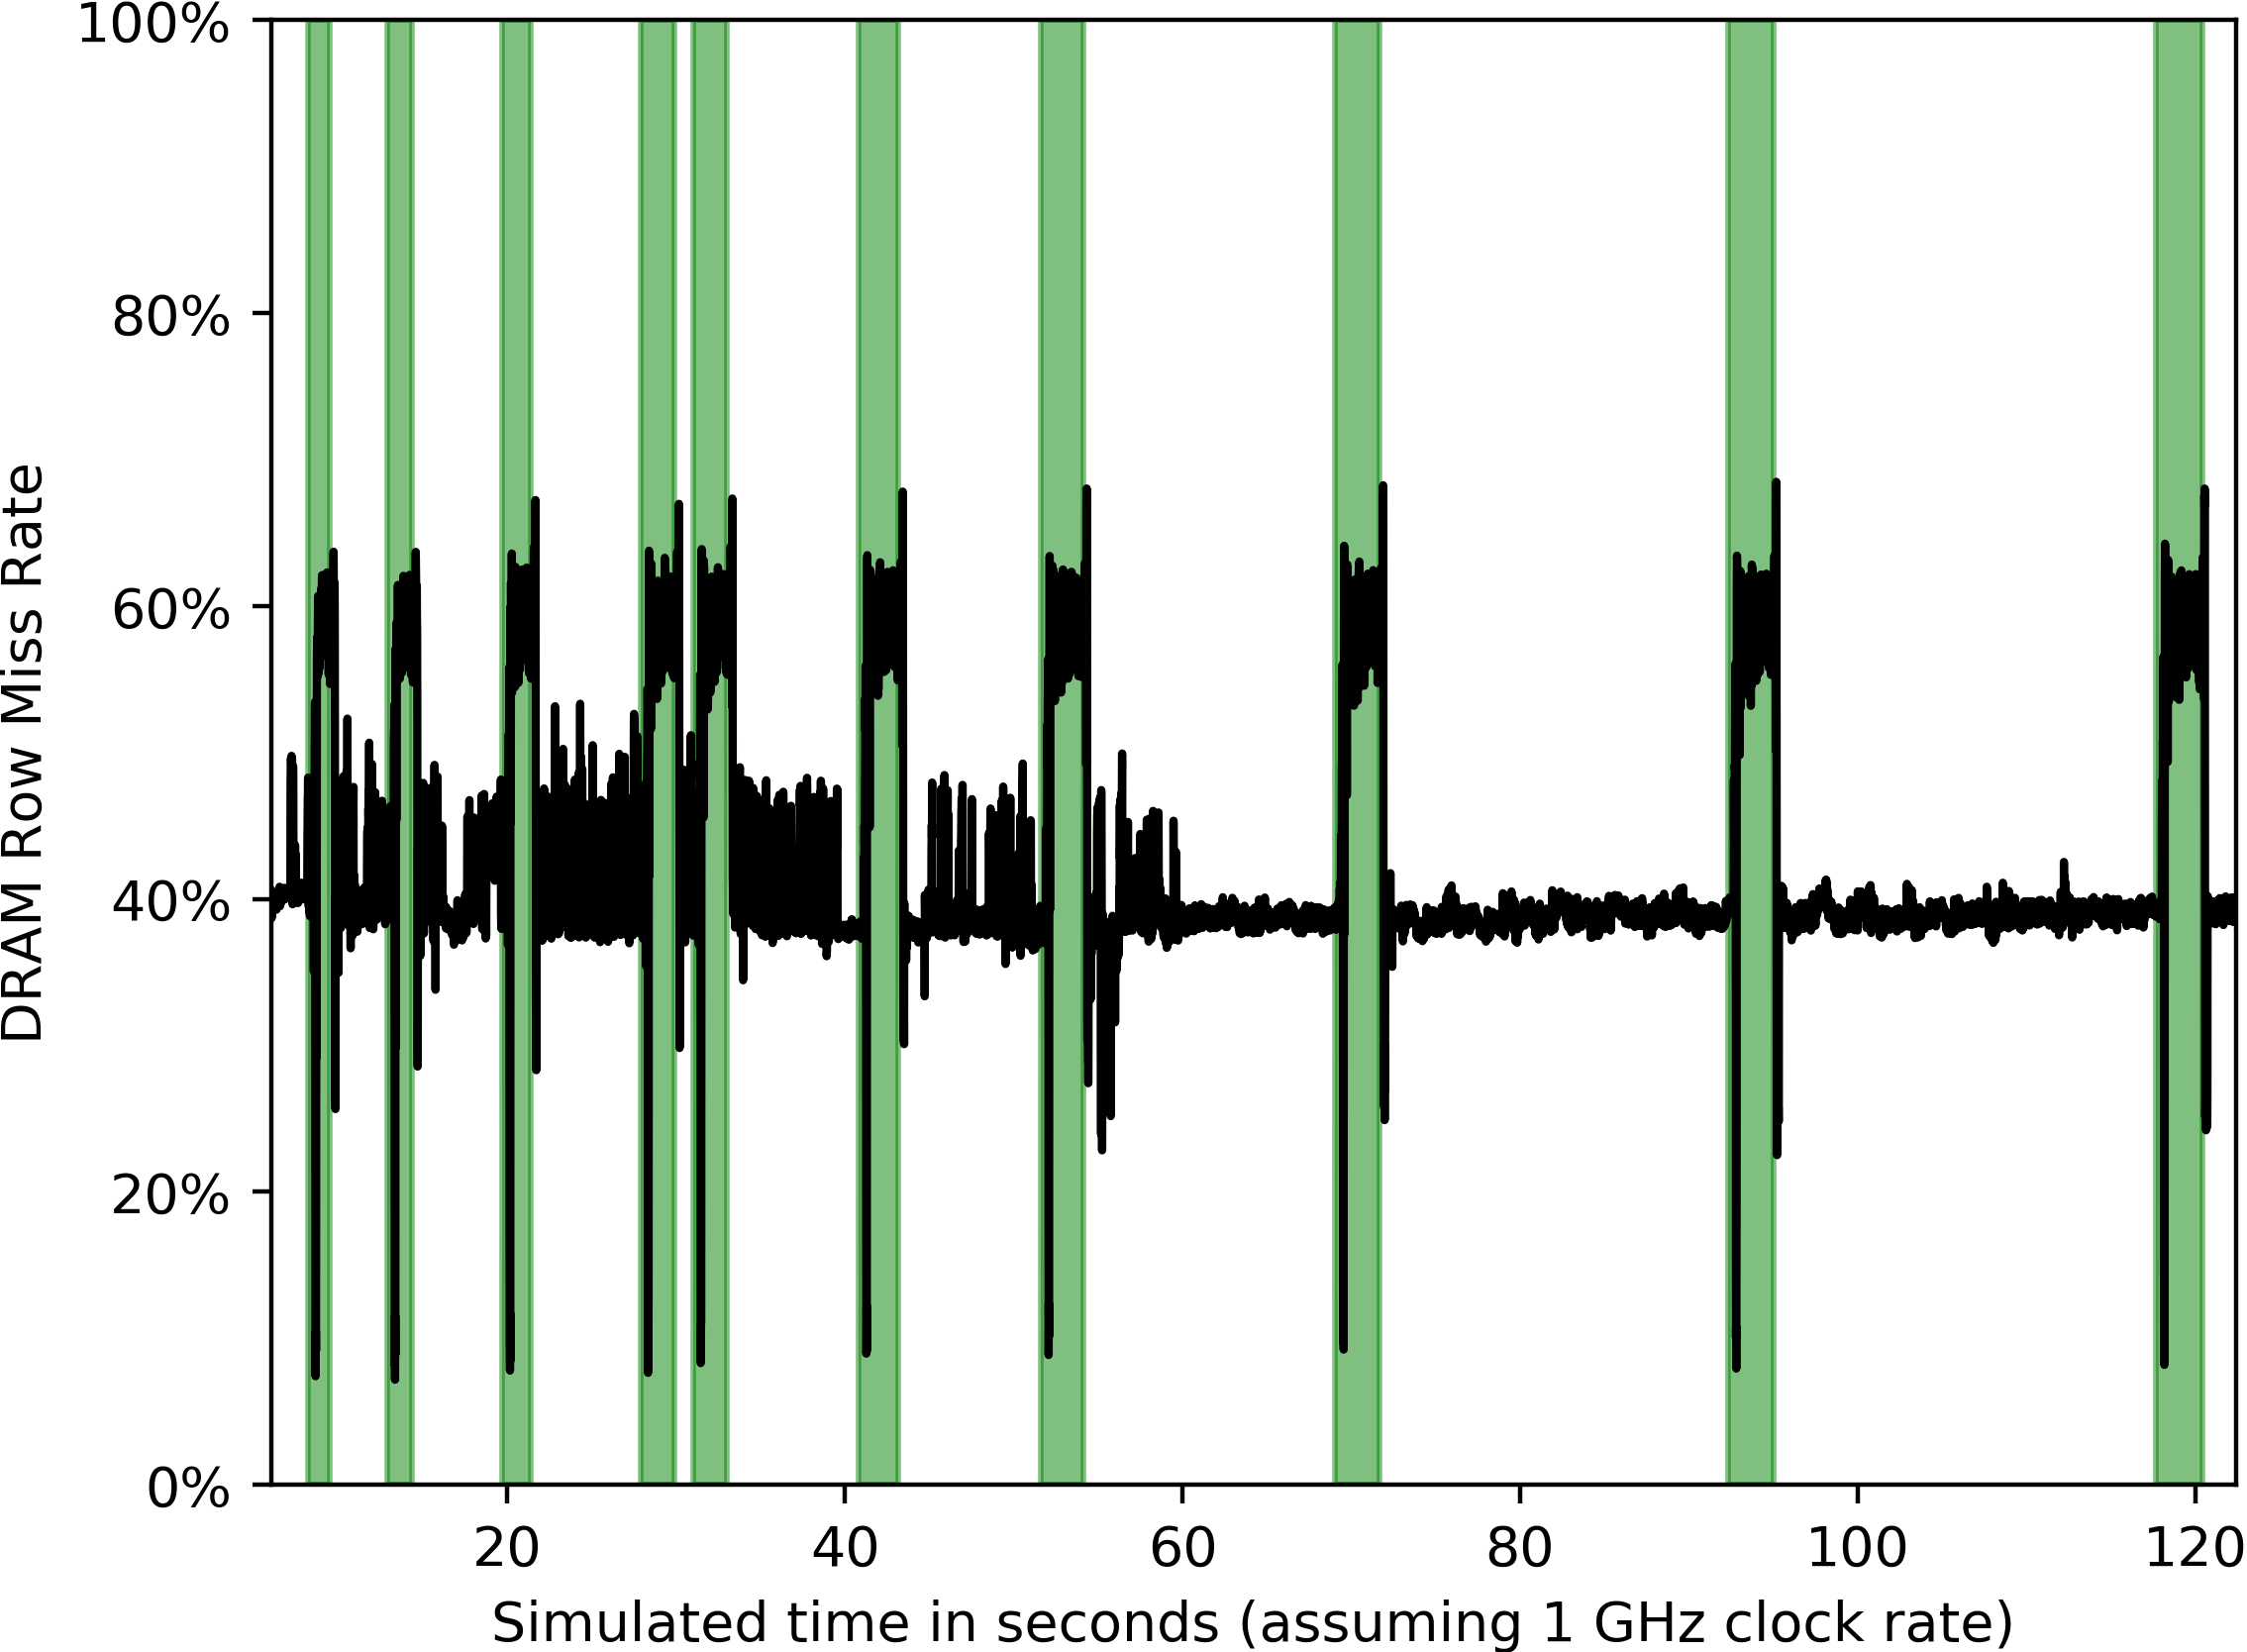
\includegraphics[width=\textwidth]{results/rowmisses_sunflow.png}
		\caption{sunflow}
	\end{subfigure}
	\begin{subfigure}[t]{0.23\textwidth}
		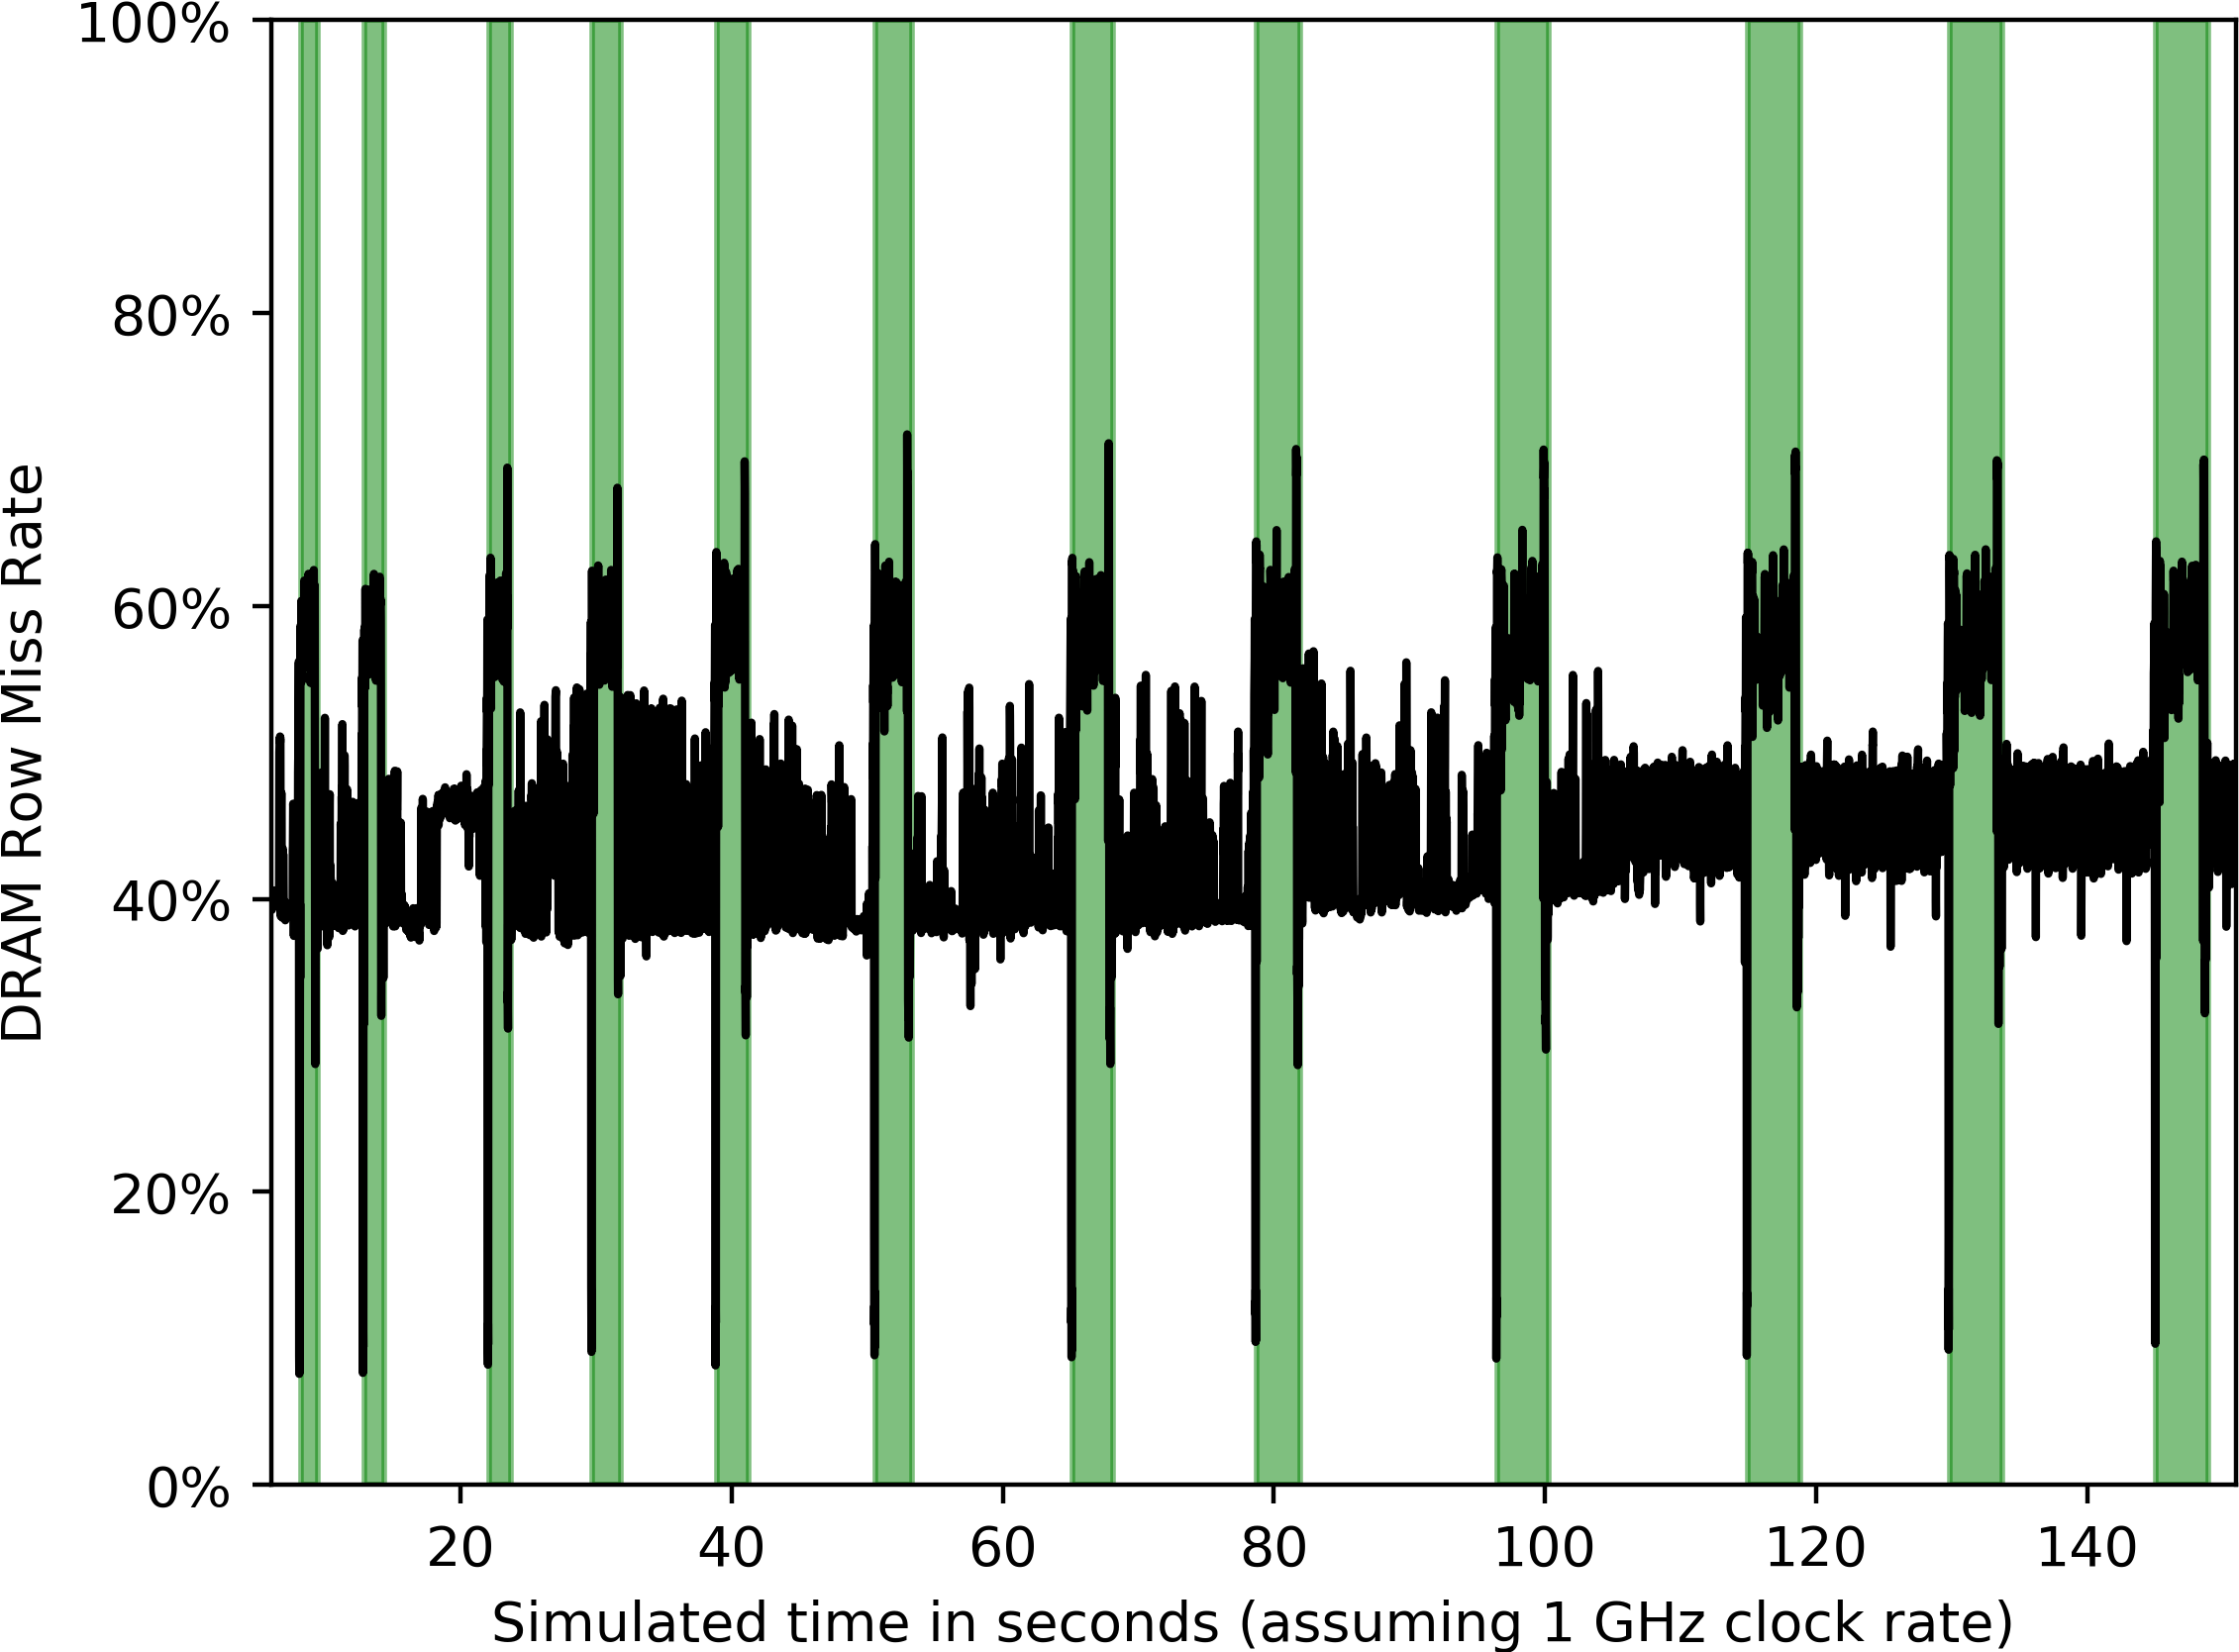
\includegraphics[width=\textwidth]{results/rowmisses_xalan.png}
		\caption{xalan}
	\end{subfigure}
	\caption{Running the Dacapo Java benchmarks and plotting the percentage of memory accesses that incur a DRAM row miss with the FCFS open-row DRAM model. While their behavior differs substantially, Garbage Collection phases are immediately visible (shown in green): due to their very low locality, they have a much lower hit rate than the rest of the application, and at the beginning of each GC phase, there is a brief period with a very high hit rate -- namely, the sequential scanning of the application's stacks to identify all references contained in them (i.e., roots).}
	\label{fig:java_rowmisses}
\end{figure*}

\subsection{High-Fidelity Application Traces}

To demonstrate the capabilities of our platform, we ran an experiment where we
annotated all memory allocation operations in JikesRVM to record a trace of
both the sizes that are being allocated and the virtual addresses that are
being returned. We buffer this (long) trace in block RAMs that we added to the
target RTL design, and read it out through automatically-inserted scan
chains~\cite{strober}.

By using this approach, we can record a trace of every memory allocation
without perturbing the execution of the program\footnote{The same mechanism
could be used to inject precomputed data, although this is currently not
implemented.}. To collect this data on a conventional system, we would need to
use either software-based sampling or code instrumentation. The latter
inherently adds observer effects and is therefore unsuitable to measure
fine-grained effects. While it was recently shown that sampling can collect
hardware-performance counters at a 1,200 cycle resolution on modern x86 cores
\cite{Yang:2015:CPM:2749469.2750401}, these approaches cannot collect
application-level details, such as allocated addresses or allocation sizes
(i.e., state contained the register file).

The fidelity of this data enables us to see effects that would be hidden by
less-detailed measurements. Figure \ref{fig:java_alloc} shows a slice of the
$\emph{pmd}$ benchmark with the time spent in allocation aggregated over
1M-cycle intervals (which corresponds to a sampling frequency of 1 KHz). While
this enables us to understand the macro-behavior of the application (Figure
\ref{fig:java_alloc}a), the data is meaningless when trying to understand the
behavior of individual memory allocations (Figure \ref{fig:java_alloc}b). In
contrast, the detailed data collected in our system (Figure
\ref{fig:java_alloc}c) shows us a much more interesting behavior: most
allocations take a small amount of time ($\approx 4,000$ cycles), while
occasional allocations take $10-100\times$ longer. This is anticipated: the
memory allocator is a segregated free list allocator and the allocator's fast
path consumes a per-size-class free list. As soon as the free list is used up,
the allocator has to fetch a new block from the global block free list, which
involves zeroing the block's memory. Dividing the allocation trace by size
class, we can measure the number of allocations to the same size class between
slow path invocations, which allows us to deduce the amount of memory
fragmentation, which would not have been visible from lower-fidelity
measurements.


Other information we can learn from this trace are allocation rates, the
distribution of allocated memory sizes and the pattern of allocated addresses:
in particular, we are often interested in the locality of subsequent memory
addresses assigned by the allocator, as this has been shown to be crucial for
performance~\cite{Blackburn:2004:OWH:998675.999420}.
Figure~\ref{fig:java_alloc_heatmap} shows the addresses generated by the
allocation, colored according to the size of the allocated object. What we can
see is that while allocation of the same object sizes is usually contiguous
(until the end of the free list is reached and a new block is acquired), the
overall temporal locality is low, confirming the conventional wisdom that
free-list allocators produce poor locality
\cite{Blackburn:2004:OWH:998675.999420}.

\subsection{Varying the DRAM Timing Model}

Managed runtime systems are often sensitive to the underlying hardware
\cite{Cao:2012:YYP:2337159.2337185}. Using our platform, it is possible to vary
the details of the underlying memory system, and explore their impact on the
application.

We ran an experiment where we measured the impact of doubling the memory
latency for the FCFS MAS timing model with open page policy from Table
\ref{tbl:fifo_mas} (Figure~\ref{fig:dacapo_latency2x}). This allowed us to
understand how sensitive different phases of the language runtime system are to
memory latencies.

These experiments taught us that the GC phase is substantially less affected by
high memory latencies than the rest of the application. This was surprising to
us, as the GC consists mainly of a pointer chase and should therefore be
strongly affected by the latency. However, upon closer investigation, we
discovered that each GC step involved not only following an object reference
but also parsing the object, identifying its outbound references and enqueuing
these references to a queue that is resident in the cache. With a trace-based
JIT-compiler, these operations would be inlined, but with a non-optimizing JIT,
they turn into a large number of function calls with high cache hit rates.

This confirms a similar result regarding non-optimized managed code by Cao et
al. \cite{Cao:2012:YYP:2337159.2337185}. We found the fact that our platform
allowed us to identify this somewhat counter-intuitive effect encouraging.

\subsection{Recording Memory System Metrics}

Finally, by running with one of our detailed memory models, we can gain deeper
insights into the application behavior than on a traditional system. To
demonstrate this, we ran several Dacapo benchmarks with the FCFS timing model
and an open-row policy. We recorded the fraction of DRAM accesses that incurred
a row miss (Figure \ref{fig:java_rowmisses}).

This exhibited an interesting effect: although each application has a very
different behavior, we can see that all benchmarks periodically exhibit a very
distinctive pattern of row miss rates: a large spike of brief, low row miss
rates, followed by a period of very high miss rates. By correlating this
behavior to the application output, we identified that these were the garbage
collection phases in the application.

Specifically, at the beginning of each GC phase, the JVM has to sequentially
scan the application's stacks and global variables, which are long, sequential
accesses that substantially benefit from an open-row policy. This is followed
by a phase of pointer-chasing -- while we saw in the previous section that many
memory accesses during this phase hit in the cache, those that do go through to
main memory rarely hit an open row, because of the very limited locality during
the tracing phase.

By using our memory model and collecting these metrics, we are able to gain
deeper insight into these kinds of effects. This could be a first step towards
modifying the memory system in order to tune it better for managed-language
workloads (e.g., to improve energy-efficiency
\cite{Cao:2012:YYP:2337159.2337185}). By allowing us to modify the memory
system model, our platform enables this kind of research.


\chapter{Conclusion}
FPGAs in the cloud provide a compelling platform to build fast, detailed
full-system simulators. However, if FPGA-accelerated simulation is to see wider
adoption, the usability limitations of prior work must be addressed.  One
promising avenue lies in automatically deriving cycle-exact, bit-exact FPGA
models from synthesizable target RTL modules. This reduces model-building and
validation effort while enabling researchers to also observe cycle-time, area,
and power impacts using commercial ECAD tools.

\PNAME addresses a longstanding hole in these RTL-transforming approaches by
providing models of outer cache hierarchies and DRAM memory systems---components
of the target design that cannot be naively transformed from ASIC
RTL.  However, by applying the same transformation on a target-time
timing-model, \PNAME obviates many of the pitfalls of handwriting FPGA-hosted
models, as it separates the concerns target-behavior modeling and
host-platform mapping. As a result, \PNAME instances are both fast---capable
of running at the host frequency---and detailed---comparable to
cycle-accurate software simulators of DRAM---while being far less onerous
to implement.

% \appendix

\printbibliography

\end{document}
